\documentclass{article}

\usepackage[utf8]{inputenc}
\usepackage[spanish]{babel}
\usepackage{fullpage}
\usepackage{hyperref}
\usepackage{graphicx}
\usepackage{mathtools}
\usepackage{amsmath}
\usepackage{sidecap}
\usepackage{listings}
\usepackage{color}
\usepackage{setspace}
\usepackage{subcaption}
\usepackage{booktabs}


\title{Informe de tesis de licenciatura}
\author{Ionatan Perez}
\date{\today}




\begin{document}

\spacing{1.5}



% Cosas del formateo para la inclusion del codigo
\definecolor{dkgreen}{rgb}{0,0.6,0}
\definecolor{gray}{rgb}{0.5,0.5,0.5}
\definecolor{mauve}{rgb}{0.58,0,0.82}
\renewcommand{\lstlistingname}{Código}
\lstset{frame=tb,
  language=Java,
  aboveskip=3mm,
  belowskip=3mm,
  showstringspaces=false,
  columns=flexible,
  basicstyle={\small\ttfamily},
  numbers=none,
  numberstyle=\tiny\color{gray},
  keywordstyle=\color{blue},
  commentstyle=\color{dkgreen},
  stringstyle=\color{mauve},
  breaklines=true,
  breakatwhitespace=true,
  tabsize=3
}




\maketitle

\clearpage 

\tableofcontents  %lo ponemos para trabajo largos que necesiten indice
\clearpage

\section{Introducción}

    Los mecanismos y dispositivos de sustitución sensorial (SSD) son técnicas en las cuales los estimulo generados en nuestro entorno y que normalmente son percibido a través de un dado sentido son reemplazados por otro estímulo (pero que codifica información equivalente) de manera que pueda ser percibido a través de un sentido sensorial alternativo. Típicamente estas técnicas son utilizadas por personas que carecen de alguno de los sentidos para poder percibir lo que de otra manera no podrían. Ejemplos cotidianos de estas técnicas son por ejemplo el bastón que suelen usar las personas ciegas, las marcas y guías en baldosas, el código braille, los timbres que encienden luces, las escalas cromáticas aptas para daltónicos, etc. 
    
    En particular, dentro de las deficiencias biológicos de percepción, el problema de la ceguera es uno que conlleva limitaciones muy importantes para las personas que la sufren y que afecta a cerca de diez millones de personas en el mundo \cite{NroCiegos}. Como paliativo a dicha situación existen diferentes técnicas (algunas de muy baja complejidad, pero funcionalidad limitada) para sustituir sensorialmente los estímulos, como puede ser un bastón que al tacto permita reconocer obstáculos. Otras técnicas, mucho mas complejas y en actual desarrollo, apuntan a restituir la capacidad de visión mediante implantes que estimulen artificialmente al sistema nervioso\cite{Implantes1,Implantes2}, pero actualmente se encuentran en un estado muy temprano de desarrollo, solo sirven en casos específicos, poseen poca resolución y son muy invasivas \cite{Implantes3,Implantes4}. 
    
    Alternativamente a las técnicas que buscan restituir la visión en personas ciegas, están las técnicas que sustituyen los estímulos, estos estímulos pueden ser reemplazados por estímulos táctiles o bien auditivos. La representación táctil de los estímulos visuales comparte la propiedad intrínseca de ser percibida en un sistema de coordenadas bidimencional (la piel y la retina ambos poseen sensores distribuidos en una superficie). Los trabajos pioneros en este técnica fueron realizados por Paul Bach-y-Rita \cite{Tactil1} quien diseñó un dispositivo que sujeto en la espalda de las personas podía reproducir imágenes filmadas por una cámara. Sin embargo la baja resolución de este dispositivo (20x20 pixeles), junto a su tamaño hicieron que sea poco practico. En posteriores trabajos \cite{Tactil2} se reemplazó el dispositivo por uno colocado en la legua (la lengua tiene una sensibilidad muy alta) donde además se reemplazó el mecanismo de estímulo por uno de pequeñas descargas eléctricas. Este trabajo solucionó en buena parte el problema de la portabilidad del dispositivo (que media 3cmx3cm con 12x12 pixeles), pero su capacidad de distinguir objetos sigue siendo reducida \cite{Tactil3}, comparable (sin entrenamiento) a 20/860 \footnote{Esta manera de indicar la capacidad visual de una persona representa cuan lejos tiene que estar (medido en pies si el numerador es 20) de dos puntos para distinguirlos en relación a una persona con visión plena. Se suele considerar a una persona con problemas de ceguera cuando su capacidad esta por debajo de 20/200}. Estudios \cite{Tactil4} muestran que con entrenamiento los sujetos pueden mejorar en cu capacidad de percepción, sin embargo hay una limitación básica en la resolución que permite este dispositivos que esta dado por la separación espacial de los electrodos y la capacidad de la lengua de distinguirlos. 
    
    \begin{figure}
        \center
        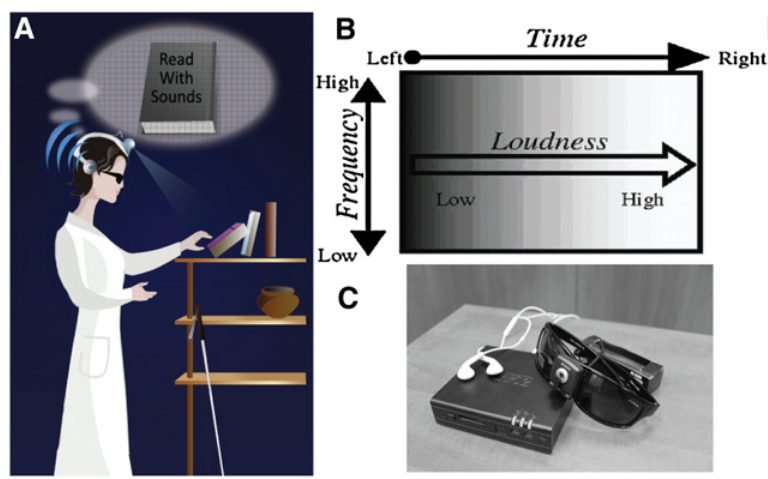
\includegraphics[width=0.8\textwidth]{Imagenes/Voice2.png}
        \caption{Dispositivo de sustitución sensorial vOICe y ejemplo de representación de las imagenes a través de dicho dispositivo. Imagen extraida de \url{http://dx.doi.org/10.1371/journal.pone.0033136}}
        \label{fig:Voice2}
    \end{figure}
    
    \begin{figure}
        \center
        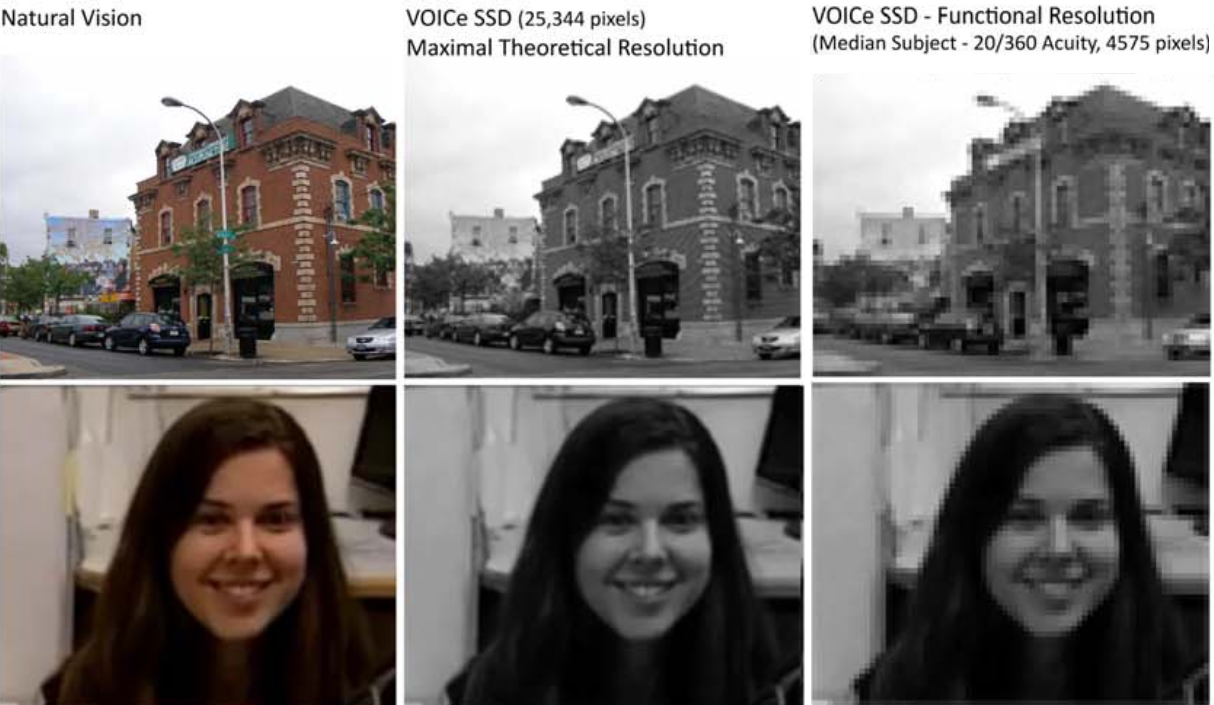
\includegraphics[width=\textwidth]{Imagenes/ImagenVoice1.png}
        \caption{En esta figura (extraída de \url{http://dx.doi.org/10.1371/journal.pone.0033136}) se compara con dos imágenes la limitación de resolución que implica el uso de vOICe. Entre la primera y la segunda se observa la pixelación inherente al algoritmo que utiliza el vOCIe, incluso asumiendo que los sujetos puedan percibir toda la información representada en los sonidos. En la derecha se observa una reconstrucción de cual es el poder de resolución que mostraron los sujetos entrenados en esta técnica.}    
        \label{fig:Voice1}
    \end{figure}
tos e    
    \begin{figure}
        \center
        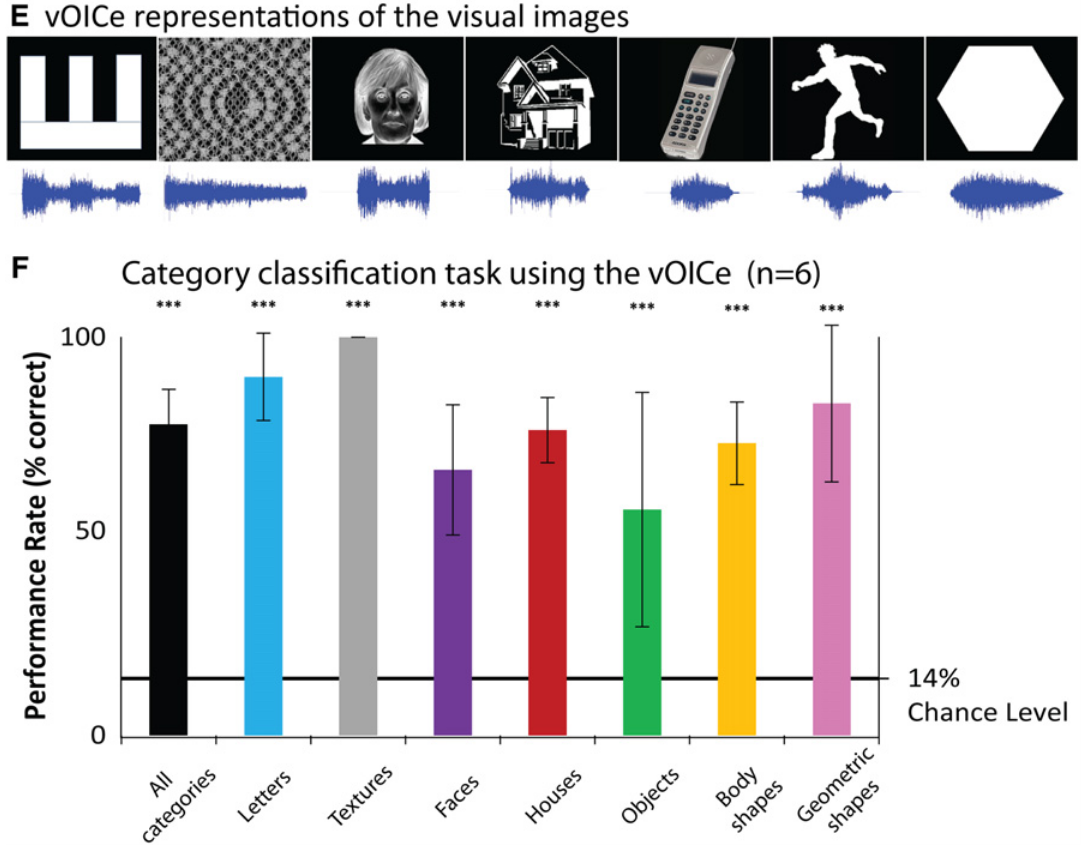
\includegraphics[width=0.7\textwidth]{Imagenes/Voice3.png}
        \caption{Ejemplo del sonido correspondiente a imágenes pertenecientes a diferentes categorías y la capacidad del distinguirlas en sujetos que fueron entrenados durante periodos de tiempo prolongado en la tecnología vOICe. Imagen y resultados extraídos de \url{http://dx.doi.org/10.1016/j.neuron.2012.08.026}}
        \label{fig:Voice3}
    \end{figure}
    
    
    El otro mecanismo por el cual se puede realizar sustitución sensorial es transformando el estimulo visual en un estímulo sonoro. El primer prototipo de esta tecnología (denominada vOICe) fue desarrollado en 1992 \cite{Voice1} como un dispositivo portátil, de bajo costo y de resolución mayor a las alcanzadas por los métodos de sustitución táctil (ver figura \ref{fig:Voice1}). Con el tiempo se fueron desarrollando versiones mejores, de mayor resolución y adaptadas a las tecnologías mas modernas (ver figura \ref{fig:Voice2}).
    
    La tecnología vOICe (\url{https://www.seeingwithsound.com/}), a diferencia de la sustitución sensorial táctil presenta la libertad de elegir que parámetros del sonido se eligen para representar los parámetros que usualmente se observan con la vista. A priori hay una amplia libertad en la elección de la representación (si se utilizan efectos sonoros complejos), sin embargo, recurriendo a las características básica del sonido hay tres grados de libertad a la hora de crear un sonido: el tono o frecuencia, el volumen y la duración. Estas tres características son las que utiliza el vOICe para representar la información visual (codificada en escala de grises). El vOICe toma una imagen, la pixela, y representa la coordenada vertical de cada pixel en la frecuencia, la coordenada horizontal en el tiempo (o duración del pixel) y la intensidad (o brillo) del pixel en el volumen o intensidad del sonido. En otras palabras lo que hace es interpretar cada columna de la imagen como una antitransformada de fourier del sonido a generar. 
    
    A partir de esta concepción de sustitución sensorial, el vOICe se fue desarrollando sobre diferentes plataformas tecnológicas siendo hoy una aplicación disponible en PCs, celulares, y otros dispositivos que sean capaces de grabar imágenes y reproducir sonidos. Además cuenta con herramientas integradas de utilidad para personas ciegas como ser comandos por vos, filtros del la imagen a procesar por color, geolocalizacion, etc. La version para celulares pude consultarse en \url{https://play.google.com/store/apps/details?id=vOICe.vOICe} y un manual para realizar el entrenamiento adecuado para su uso en \url {https://www.seeingwithsound.com/manual/The_vOICe_Training_Manual.htm} 
    
    Además del desarrollo de la tecnología vOICe como aplicación, se realizaron otras pruebas e investigaciones sobre esta tecnología. Una es la denominada PSVA \cite{VoiceVariante1}, esta difiere del vOICe en que la escala vertical esta discretizada no en función de la resolución como numero de pixeles, sino utilizando saltos que difieran en notas fijas, además posee una región de mayor resolución en la zona central de la imagen, simulando el funcionamiento del ojo. Otra variante es el denominado SmartSight que filtra y agrupa secciones de la imagen antes de realizar una representación sonora en forma de notas musicales \cite{VoiceVariantes2, VoiceVariantes3}. También se esta desarrollando una versión similar el vOICe denominada EyeMusic que codifica en términos de notas la altura de los pixeles, pero utilizando diferentes instrumentos para representar diferentes colores de manera de poder ofrecer a los no videntes una sustitución sensorial que incluya este aspecto de la visión natural.\cite{VoiceVariantes4}.
    
    En otro sentido, a partir del imágenes y mediciones de actividad cerebral y de entrenamiento se han realizado estudios acerca del funcionamiento subyacente al mecanismo de sustitución sensorial. Hay estudios que muestran que en el caso de personas ciegas de nacimiento se activas zonas típicas de procesamiento de la información para el canal sensorial utilizado, mientras que en personas que perdieron la visión siendo adultos se activan zonas del procesamiento de imágenes (frente a un mismo estimulo), o que la modulación de la actividad cerebral difiere entre personas que perdieron la vista a edad temprana y personas que simplemente reciben el estimulo teniendo la vista tapada \cite{VoiceSubyacente1,VoiceSubyacente3}. También hay estudios que muestran que con entrenamiento los sujetos aprenden a reconocer patrones e incluso pueden transferir el aprendizaje entre figuras similares \cite{VoiceSubyacente2}. Por otro lado estudios sobre la tecnología vOICe muestran que los sujetos son capaces de entrenar e integrar la percepción en tareas de reconocimiento de geometría espacial, siendo capaces de ubicar y señalar posicionamiento de objetos en un entorno 3D donde pueden cambiar el punto de vista de la cámara con la que observan los estímulos \cite{VoiceSubyacente4}
    
    Volviendo a los estudios sobre la tecnología vOICe en su concepción más original y sencilla, que es sobre la que se decidió trabajar, los estudios previos muestran que los sujetos entrenados (que pueden ser tanto ciegos como videntes\cite{VoiceEntrenamiento1}) pueden aprender a distinguir entre categorías de imágenes complejas \cite{VoiceEntrenamiento2} (como los que se observan en la figura \ref{fig:Voice3}). Con este antecedente, nosotros en nuestro trabajo intentamos estudiar la capacidad no de interpretar figuras complejas, sino sencillas, pero en términos de categorías geométricas. 
    
    La idea detrás de la propuesta fue que, si bien a la hora de interactuar con entornos complejos es importante que el sistema de sustitución sensorial permita representar de forma equivalente información compleja, muchas actividades no requieren interactuar con estímulos complejos. Muchas veces los estímulos o bien son intrínsecamente sencillos (por ejemplo los iconos y contornos en la navegación dentro de una computadora) o bien se puede preprocesar la imagen para extraer con algoritmos las información mas relevante antes de realizar la sustitución sensorial. Por otro lado, estudiar la capacidad de detectar conceptos geométricos abstractos podría permitir inspeccionar, dentro de la compleja tarea de reconocer patrones, que aspectos son mas difíciles de identificar, cuales mas fáciles, y de que depende la dificultad a la hora de interpretar geometría en este contexto. 

\section{Objetivos generales y breve panorama del trabajo realizado} \label{seccion:panorama}

    El objetivo general detrás del trabajo realizado fue estudiar la capacidad de los sujetos de percibir información geométrica a través de un sistema de sustitución sensorial tipo vOICe, observar de que parámetros depende dicha capacidad, y estudiar posibles transferencia del aprendizaje realizado frente a transformaciones de simetrías (en principio reflexiones y rotaciones). 
    
    Para realizar esta tarea se quiso diseñar un protocolo experimental en el que los sujetos fueran expuestos a estímulos y debieran detectar en ellos algún aspecto geométrico, luego a un subgrupo de los sujetos medidos se los entrenaría en alguna categoría especifica, y por último se volvería a medir en todos los sujetos su capacidad de detectar los patrones geométricos en una medición equivalente a la inicial. Comparando los desempeños obtenidos en ambas mediciones se podría estudiar por un lado la capacidad de percibir aspectos geométricos en función de las características de los estímulos presentados y por otro observar el posible efecto del entrenamiento en esa capacidad. Este fue el objetivo general, en función del cual se realizó todo el trabajo así como los sucesivos diseños experimentales. 
    
    En los hechos, resultó que la mayor parte del trabajo realizado estuvo enfocado en la construcción de las herramientas (básicamente algoritmos y programas) necesarias para hacer los experimentos, así como la caracterización de las limitaciones experimentales relacionados con los métodos utilizados o bien inherentes al método de sustitución sensorial en el marco del cual se busco realizar las mediciones. Para realizar las mediciones se decidió utilizar como sujetos a personas videntes ya que resultados previos\cite{VoiceEntrenamiento3} indicaban que tanto ciegos como videntes pueden ser entrenados en la tecnología vOICe con resultados similares, y de esta forma se evitaban todas las limitaciones y complicaciones que implicarían hacer experimentos con personas no videntes.
    
    Respecto a los problemas experimentales a resolver para poder realizar los experimentos, resultaron muy diversos, pero se pueden englobar en los siguientes puntos conceptuales: 
    
    \begin{itemize}
        \item Diseñar un algoritmo que creara secuencias de estímulos en forma sistemática y paramétrica adecuadas para probar las hipótesis de cada diseño experimental. 
        \item Adaptar, caracterizar y testear un algoritmo compatible con el resto del código que transformara los estímulos en su correspondiente representación sonora, y que respondiera a la lógica del vOICe. 
        \item Diseñar los experimentos que quisiéramos realizar y en función de ello generar los estímulos y niveles (instrucciones para crear un conjuntos de pruebas consecutivas con las especificaciones necesarias) adecuados.
        \item Diseñar la lógica de ejecución en tiempo real mediante la cual el experimento adapta los estímulos a mostrar en función de las respuestas de los usuarios (esto fue particularmente importante en las últimas mediciones)
        \item Diseñar una aplicación que fuera capaz de interpretar e integrar en una interfaz con el usuario toda la información relacionada a los estímulos y niveles creados, manejando en tiempo real la elección de estímulos y parámetros según correspondiera, así como el correcto registro de múltiples indicadores que permitieran luego reconstruir por completo lo realizado por el sujeto experimental. 
        \item Procesar los datos registrados para validar las hipótesis de los diseños experimentales y proponer adaptaciones o cambios en al mismo. 
    \end{itemize}
    
    Resolver cada uno de estos aspectos (donde se omitió todas las pruebas preliminares realizadas) implicó una gran cantidad de decisiones, pruebas y elecciones que si bien correspondían a una de las categorías mencionadas muchas veces estaban motivadas o limitadas por decisiones adoptadas en otra de las categorías. El trabajo realizado consistió en un continuo desarrollo y adaptación de algoritmos mutuamente relacionados donde realizar un raconto temporal de lo hecho seria confuso y carente de sentido. Por esa razón elegimos como criterio a la hora de presentar el trabajo realizado, presentar un breve resumen conceptual de la evolución general de los objetivos, detallar luego el trabajo y la evolución realizada en cada aspecto de las herramientas desarrolladas para realizar los experimentos y por último presentar los resultados obtenidos en las mediciones realizadas. 
    
    En términos temporales el primer desafío que se propuso fue hacer un experimento en el que pudiéramos saber si los usuarios eran capaces de distinguir figuras geométricas, para ello pensamos en segmentos paralelos o no paralelos, ángulos rectos o no rectos y cuadriláteros cuadrados o no cuadrados (esto últimos son una combinación de las dos categorías anteriores y permitirían evaluar procesos de transferencia). El resultado (luego de muchas pruebas preliminares, ajustes, calibraciones y horas de programación) fue satisfactorio en tanto los sujetos eran capaces de interpretar al menos en términos muy básicos las figuras geométricas (generadas con parámetros variados al azar) y distinguir entre grandes categorías o ejemplos muy diferentes. Esto no era obvio que fuera a suceder ya que los trabajos previos requerían decenas de horas de entrenamiento mientras que nuestros experimentos tenían que involucrar tiempos mucho más cortos.
    
    Sin embargo surgieron dos problemas a la hora de pensar en un proceso de entrenamiento o medición mas cuidadoso. En primer lugar resultó evidente que la representación sonora es fuertemente no invariante frente a rotaciones, es decir que es clave la orientación de los segmentos que conforman las figuras a la hora de establecer la dificultad de interpretarlos y esta dependencia no la teníamos caracterizada. Por otro lado no teníamos ningún parámetro de la dificultad para cada estímulo en particular, por lo tanto no teníamos manera de armar un conjunto de estímulos que de alguna manera pudieran distinguir la capacidad de los sujetos en la zona de parámetros donde no saturara la medición como muy fácil o muy difícil. 
    
    Cabe aclarar que todas las mediciones de esta primer etapa se realizaron en forma esporádica y sin llevar un protocolo unificado que permitiera extraer conclusiones o resultados numéricamente validos. Por esto, cuando ya se contaba con una versión de la aplicación bastante funcional y una noción de las dificultades a superar se decidió realizar un primer experimento piloto en el cual medir como variaba la dificultad de reconocer una propiedad de los estímulos según la orientación del mismo. Este experimento implicó definir y ajustar varias cuestiones relacionadas al diseño experimental y los algoritmos necesarios para implementarlo. El primero y mas importante fue que en lugar de distinguir entre categorías para estímulos aleatorios (los mismos para todos los sujetos) necesitábamos caracterizar la capacidad de los sujetos en una tarea especifica y para eso era necesario realizar un experimento tipo Quest con el cual medir un umbral de detección. 
    
    Este cambio requería por un lado generar secuencias de estímulos similares que variaran en una única dimensión o parámetro de manera de poder fluctuar dicho parámetro hasta encontrar el punto donde el usuario pasara de distinguir el aspecto evaluado del estimulo a no distinguirlo. Por otro lado requería adaptar la lógica de funcionamiento de la aplicación y de los niveles para que pudieran ajustar la dificultad del estimulo mostrado en tiempo real en lugar de repetir una secuencia preestablecida. Además en la realización de este experimento pusimos a prueba todas las dificultades inherentes a la logística de realizar un experimento en laboratorio siguiendo un protocolo formal.
    
    Los resultados de este experimento mostraron que efectivamente la dependencia de la dificultad con la orientación existía y era muy marcada, pero también mostraron que había una enorme variabilidad intersujeto por lo cual no tenia sentido establecer la dificultad de un estimulo como parámetro intrínseco del estímulo. Por otro lado en este experimento descartamos evaluar los cuadriláteros por poseer mas de un parámetro a evaluar en simultaneo y por lo tanto ser incompatibles con el diseño experimental. Decidimos evaluar las categorías de paralelismo ("paralelas"/"no paralelas") y de ángulos ("agudo"/"recto"/obtuso"). Habiendo avanzado hasta este punto, la idea de medir y realizar entrenamiento con estímulos genéricos y comunes a todos los sujetos (como habíamos pensado en un principio) resultaba inviable pues cada sujeto reportó una capacidad de percepción muy diferente a los demás. 
    
    Por ello ideamos un último experimento donde lo que se buscaría observar era si el entrenamiento en alguna condición especifica producía una mejora en el desempeño del sujeto durante y luego del entrenamiento, y si se puede observar una transferencia de dicha mejora entre las condiciones evaluadas. Para eso se diseñó un protocolo en el cual se mediría el desempeño inicial de los sujetos, luego a algunos sujetos se los entrenaría (dándoles feedback acerca de sus respuestas) en la detección de ángulos, a otros en la detección de paralelas y a otros no se los entrenaría. Por último se volvió a medir el desempeño de todos los sujetos con la intención de poder comparar el efecto del entrenamiento. 
    
    Como parte de los cambios realizados en este protocolo, se mejoró el mecanismo de medición del umbral respecto al experimento anterior, se eligió un conjunto de configuraciones o niveles con un alto grado de simetría con el objetivo de distinguir si la posible transferencia dependía de algunos de estos invariantes, y se seleccionó las orientaciones donde los sujetos mostraban peor desempeño inicial con el objetivo de tener un mayor rango donde medir posibles efectos de mejora. 
    
\section{Desarrollo de las herramientas necesarias}

\subsection{El proceso de creación de estímulos} \label{seccion:SVG}
    
    El proceso de creación de estímulos implicó dos desafíos, por un lado disponer de alguna lógica, paramétrica de creación de figuras geométricas que sirvieran para testear las hipótesis y por otro el de transformar los estímulos creados en términos visuales o geométricos a su representación sonora. Mientras que el primer aspecto requirió una constante adaptación y sofisticación en función de los cambios experimentales, el segundo fue resuelto al inicio de trabajo y la solución, con leves cambios sirvió para todas las pruebas y experimentos realizados. 
    
    La lógica del vOICe para transformar imágenes en sonidos es muy sencilla y genérica, de ahí su potencialidad para representar cualquier tipo de figura. Para la transformación lo que hace es partir la imágen en una cuadricula de NxM donde cada elemento se corresponde con un pixel en la imagen y a partir de esta matriz se genera el sonido a reproducir. Para ello, se considera el índice vertical (lo llamaremos i) de la matriz como el índice que recorre las frecuencias que se debe reproducir y el índice horizontal (llamado j) indica en que tiempo de debe reproducir dicho elemento. En términos matemáticos es hacer una antitransformada de fourier usando cada columna como el espectro que corresponde a tiempos sucesivos. Esta operación (ejemplificada solo para una única imagen) se puede calcular como el resultado de la ecuación \ref{ec:VoiceOriginal} donde T representa el tiempo total que dura cada imagen. Este algoritmo se puede interpretar visualmente en la figura \ref{fig:VoiceOriginal}
    
    \begin{figure}
        \center
        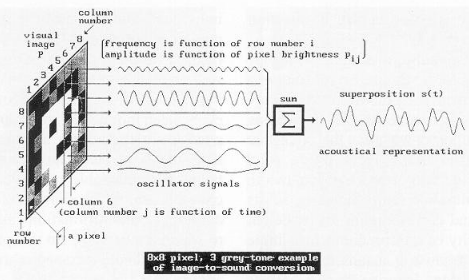
\includegraphics[width=0.5\textwidth]{Imagenes/VoiceOriginal.png}
        \caption{Ejemplo de representación sonora para el dispositivo original del vOICe correspondiente a la ecuación \ref{ec:VoiceOriginal}. Figura extraída de \cite{Voice1}}
        \label{fig:VoiceOriginal}
    \end{figure}
    
    \begin{equation}
        \label{ec:VoiceOriginal}
        s(t) = \sum_{i,j}^{M,N} p_{i,j} \cdot sin(w_i \cdot t + \phi) \cdot [\Theta(j \cdot T/N) \cdot (1-\Theta((j+1)T/N)]
    \end{equation}

    Con este procesamiento en mente se construyó un primer algoritmo que realizara dicha transformación y se analizó como resultaba la representación sonora para imágenes de prueba construidas con cualquier editor de gráficos. Aparecieron problemas de inmediato. Lo primero observado fue que si bien el sistema de transformación a priori no posee una limitación de resolución obvia, cuando la resolución es alta aparecen ruidos inherentes a los saltos en la discretización de la imagen. La discretización en la coordenada horizontal produce que el espectro puro correspondiente a un pixel en realidad adquiera armónicos producto de que el pixel comienza y termina en un lapso corto de tiempo. Por lo tanto cuanto mayor sea la resolución mas seguido aparecen saltos de intensidad que se corresponden con la inclusión de chasquidos en el sonidos que distorsionan el sonido deseado. 
    
    Por otro lado la discretización vertical de la imagen hace que al utilizar resoluciones altas se creen secuencias de sonido de frecuencia muy similar que generan efectos de batido. Nuevamente, al incrementar la resolución utilizada estos problemas se acentúan. 
    
    
    \begin{figure}
        \center
        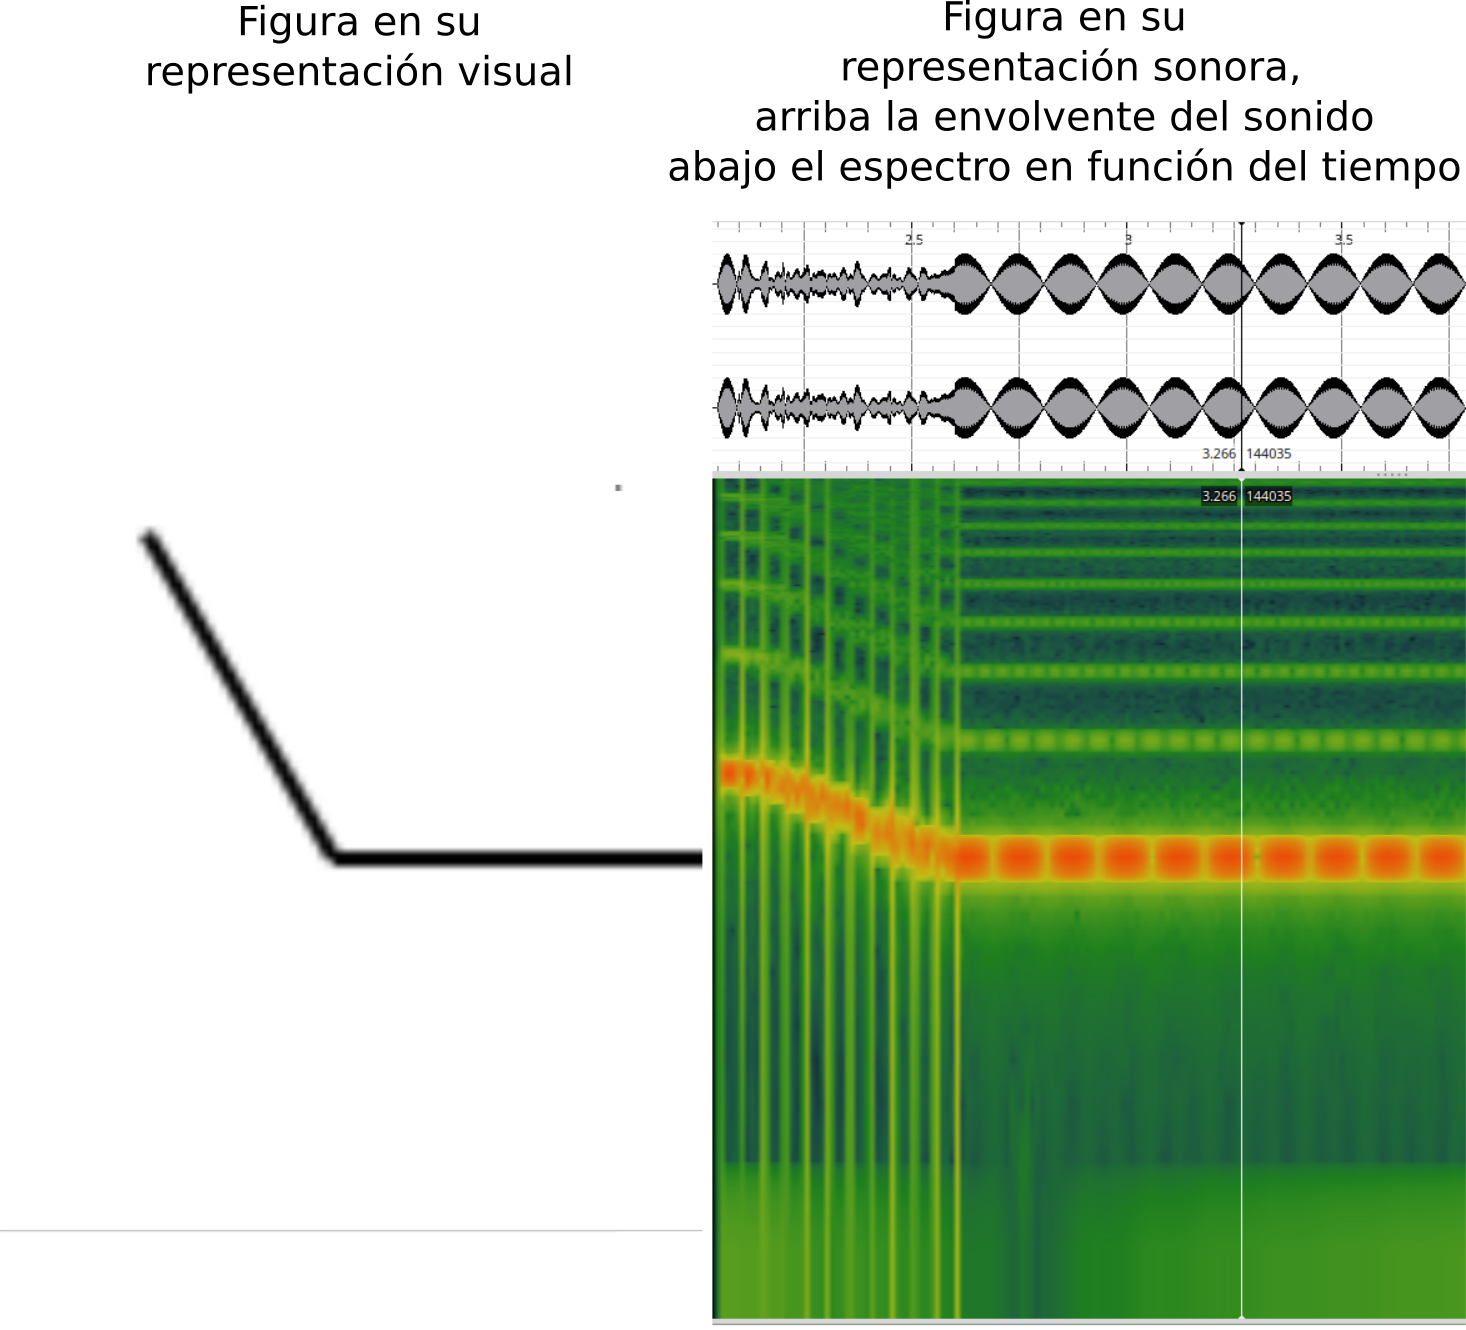
\includegraphics[width=\textwidth]{Imagenes/vOICeOriginal.png}
        \caption{Representación sonora de los estímulos utilizando la lógica de conversión del vOICe original, como la ejemplificada en la figura \ref{fig:VoiceOriginal}. Se observa los problemas de batido y la discretización de los salto en frecuencia junto con los armónicos que esto genera.}
        \label{fig:vOICeOriginal}
    \end{figure}
    
    \begin{figure}
        \center
        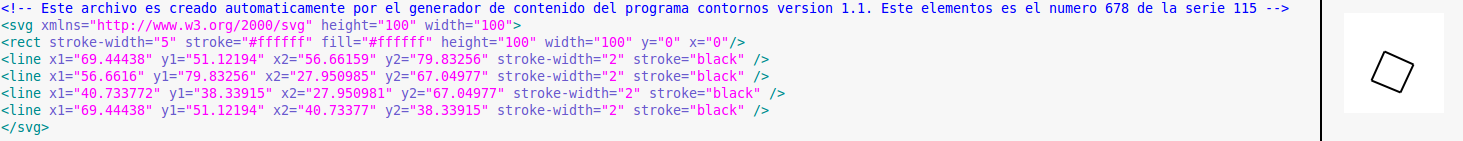
\includegraphics[width=\textwidth]{Imagenes/678SVG.png}
        \caption{Ejemplo de representación en código SVG de una figura de las utilizadas. Se observa que se trata de una variante de código XML. En el comentario inicial se almacena información acerca del contexto del algoritmo que lo crea. Luego se establece el estándar SVG y el tamaño del lienzo. Dentro, se pinta el fondo, y sobre él se agregan las lineas indicadas con las coordenadas de sus extremos. A la derecha se puede observar una representación visual del contenido.}
        \label{fig:SVGtoPNG}
    \end{figure}
    
    Estos dos problemas (que se observan en la figura \ref{fig:vOICeOriginal}), en un sistema de representación de imágenes complejas pueden pasar más desapercibidos o generar pocas alteraciones. En nuestro caso representaban un impedimento fundamental para utilizar el algoritmo original de vOICe, porque no solo impediría utilizar una representación de alta resolución sino que también incluiría en el sistema de representación un elemento indeseado que presenta una muy fuerte ruptura de simetría. Como el objetivo de nuestro trabajo estaba centrado en determinar la sensibilidad de los sujetos a aspectos geométricos y desconocíamos el rango de sensibilidad que se esperaba medir, basar todos los experimentos en una representación que a priori presenta una limitación tan evidente carecía de sentido. 
    
    Se tuvo por lo tanto que reformular el algoritmo de transformación de imágenes a sonido de manera de evitar estos inconvenientes. Hacia falta un algoritmo que respetara la representación donde a mayor altura mayor frecuencia, pero que no tuviera los problemas inherente a la discretización en pixeles de las imágenes usuales. En otras palabras hacia falta un sistema que preservara la información conceptual de los segmentos con los que queríamos construir geometría sin pasar por la instancia de representación en formato pixelado. Y también un algoritmo para transformar dicha información a una imagen visual y a su representación sonora. Esto representaba dos nuevos desafíos, por un lado generar u manipular imágenes en formato vectorial (que es un formato donde se guarda la información independientemente de su representación) y por otro poder transformar esta información vectorial en los sonidos correspondientes en forma directa (sin pasar por la imagen). 
    
    Para la primera de las dos tareas se utilizó imágenes en formato SVG. El formato SVG es un estándar de representación (\url{https://www.w3.org/TR/SVG/}) para construir imágenes a partir de información vectorial con alto nivel de difusión y fácil codificación. Tiene la ventaja de que la mayoría de los navegadores y sistemas operativos modernos son capaces de mostrar como imagen este tipo de archivos, que (al igual que los demás formatos vectoriales) permite almacenar información de una imagen arbitrariamente grande y compleja en pocas lineas de texto, de ser un estándar para el cual existen librerías en la mayoría de los lenguajes de programación capaces de manipularlo, y de ser un formato fácilmente legible incluso por humanos mirando el código fuente. En nuestro caso un factor importante a la hora de utilizar este formato fue que la elección era compatible con generar posteriores procedimientos experimentales que pudieran ser validados en contextos y dispositivos diferentes, conservando la información fundamental y conceptual de los estímulos utilizados. Un ejemplo de como se genera y visualiza la información en este formato puede verse en la figura \ref{fig:SVGtoPNG} donde se muestra la representación para una de las figuras utilizadas en las pruebas preliminares. 
    
    El código para generar estos archivos fue variando según la etapa de desarrollo experimental de manera de ser cada vez más paramétrico y automatizado. El detalle de los parámetros utilizados en los últimos experimentos se comenta mas adelante, pero para las pruebas preliminares se generaron largas secuencias de figuras incluidas en las categorías de cuadriláteros, paralelas y ángulos donde se generaban fluctuaciones aleatorias sobre los ángulos formados, las separaciones y tamaños de las lineas, y las ubicaciones en el lienzo. Luego con estas imágenes ya creadas se seleccionaba para su utilización algunas que se adecuaran a los test a realizar.
    
    Algo que se implemento también en paralelo con la generación de los archivos SVG en si mismo, fue la creación de un archivo por imagen con un registro de las características de la figura generada en formato Json \footnote{Json \url{https://es.wikipedia.org/wiki/JSON} es un estándar para almacenar contenido de variables o estructuras de datos alfanuméricas en formato texto} para que el software supiera interpretar el contenido de cada figura durante su ejecución. Junto a cada imagen se guardó las categorías geométricas a las que pertenecía dicha imagen (esto es fundamental para que el software pudiera reconocer si las respuestas indicadas por el usuario eran correctas o equivocadas), sus propiedades y parámetros geométricos con los que se la construyó (esta información queda registrada en los logs de las respuestas para que después se pueda corresponder el comportamiento del usuario en función de los valores con que se parametrizó la figura), y además se incluyo campos descriptivos a los efectos de facilitar la revisión del correcto funcionamiento del código y la detección de eventuales errores durante la fase de testeo. 
    
    Tambien, dado que el lenguaje utilizado para construir la aplicación con la que se realizaron los experimento no soportaba el uso de archivos SVG en tiempo real por ser algo poco eficiente en termino de uso de recursos se incluyó en el proceso de creación de los archivos SVG la creación de las correspondientes imágenes y su posterior agrupamiento (por niveles) en archivos ATLAS que es un formato optimizado para el uso de memoria y procesador en tiempo de ejecución.
    
    En cuanto a la tarea de construir un algoritmo que transformara las figuras geométricas en sonido, lo primero que se hizo para limitar el problema fue restringir el problema a segmentos rectos que se debían corresponder con rampas en frecuencia.
    
    Transformar el archivo SVG en un archivo de audio requería solucionar las siguientes tareas:
    
    \begin{itemize}
        \item Extraer del archivo SVG la informacion de cada linea a crear
        \item Transformar los parámetros x e y correspondientes a extremos geométricos de cada linea en parámetros de tiempo y frecuencia correspondientes los extremos de la rampa de sonido.
        \item Crear la rampa de sonido correspondiente a cada segmento
        \item Componer y normalizar correctamente el conjunto de rampas para conformar una secuencia de bits que represente la información sonora completa correspondiente a la imagen
        \item Transformar la secuencia de bits en un archivo MP3 utilizable por el resto del software
    \end{itemize}
    
    Para la extracción de la información correspondiente a cada linea, se utilizó una librería existente en Java (lenguaje en el que programamos todo el resto de la aplicación) que permite recorrer la información de archivos XML\footnote{SVG es una variente de XML}, una vez extraída la información de los extremos de cada segmento y el tamaño del lienzo, se debió implementar los siguientes chequeos y procesamientos:
    
    \begin{itemize}
        \item Revisar que la información este ordenada correctamente, es decir que primero este el extremo izquierdo y luego el derecho, en caso de que no, alternarlos. 
        \item Revisar que los extremos de los segmentos se encontraran dentro del lienzo, ya que esto no tiene porque suceder si la imagen fue creada mal (a veces algunas combinaciones de parámetros mal diseñados pueden dar que un segmento exceda exceda el tamaño del lienzo). En este caso de detectar que el segmento excede el lienzo el código además de generar una advertencia se debe recorta el segmento para que este incluido íntegramente en el lienzo.
        \item Realizar un cambio de escala según correspondiera a la configuración de como interpretar los tamaños. Esta funcionalidad nunca la utilizamos, pero al diseñar en términos conceptuales la representación sonora existía la libertad de establecer una escala de tamaño para el lienzo o para el pixel, en otras palabras no es lo mismo interpretar que un lienzo de 100x100 (tamaño usado) representa todo el espacio porque cada pixel representa un centésimo del espacio a interpretar a que cualquier imagen sin importar su tamaño en pixeles deba abarcar todo el espacio disponible. 
    \end{itemize}
    
    Una vez obtenida las coordenadas espaciales de los extremos del segmento a transformar se debía encontrar los correspondiente valores de tiempo y frecuencia para cada extremo. Para los valores temporales la cuenta se sencilla pues es lineal, por lo que la transformación esta dada por la ecuación \ref{ec:xTot}. Para los valores de frecuencia la cuenta debe incluir la elección de la escala a utilizar, que en el caso de las frecuencias no tiene porque ser lineal, pues el oído no interpreta en una escala lineal las frecuencias. Dado que el oído interpreta en escala logarítmica se decidió respetar esta escala incluyendo en el código la opción de utilizar una escala lineal. El conjunto de opciones y parámetros utilizados en todo el proceso de transformación puede observarse en el cuadro \ref{code:Constantes}

    \spacing{1}
    \begin{minipage}{\textwidth}
    \begin{lstlisting}[caption=Constantes y parámetros utilizados en el código que crea transforma la información geométrica en el estímulo sonoro., label=code:Constantes]
    
    
    // Define algunas constantes
	public final static boolean logScale = true;
	public final static boolean fixScale = true;
	public final static float maxHeigth = 100;
	public final static float frecMax = 4000;
	public final static float frecMin = 100;
	public final static float time = 5; // in secs
	public final static boolean fixedTime = true; // indicate if the length of sound must be the variable time
	public final static float secByPix = 5 / 100f; // indicate how many sec are represented by pixel.
	public final static int fs = 44100; // hz of the sound
	public final static float base = 10; // base of the log scale
    
    \end{lstlisting}
    \end{minipage}
    \spacing{1.5}
    
    Con la idea de aprovechar la mayor parte del espectro audible en un principio se decidió utilizar el rango de los 100 a los 8000 Hz, sin embargo este rango resultó un tanto excesivo en el uso de los agudos creando sonidos molestos a la hora de realizar los experimentos, por lo que se decidió hacer ingeniería inversa sobre la tecnología vOICe midiendo el espectro de frecuencias que dicha tecnología utilizaba. Como limite superior de frecuencia el vOICe utilizaba 4000 Hz, un valor que efectivamente resultó mucho más razonable y amigable al usuario. El límite inferior no se pudo detectar al realizar el espectro sobre el vOICe por lo que se mantuvo el valor de 100 Hz utilizado originalmente. 
    
    \begin{figure}
        \center
        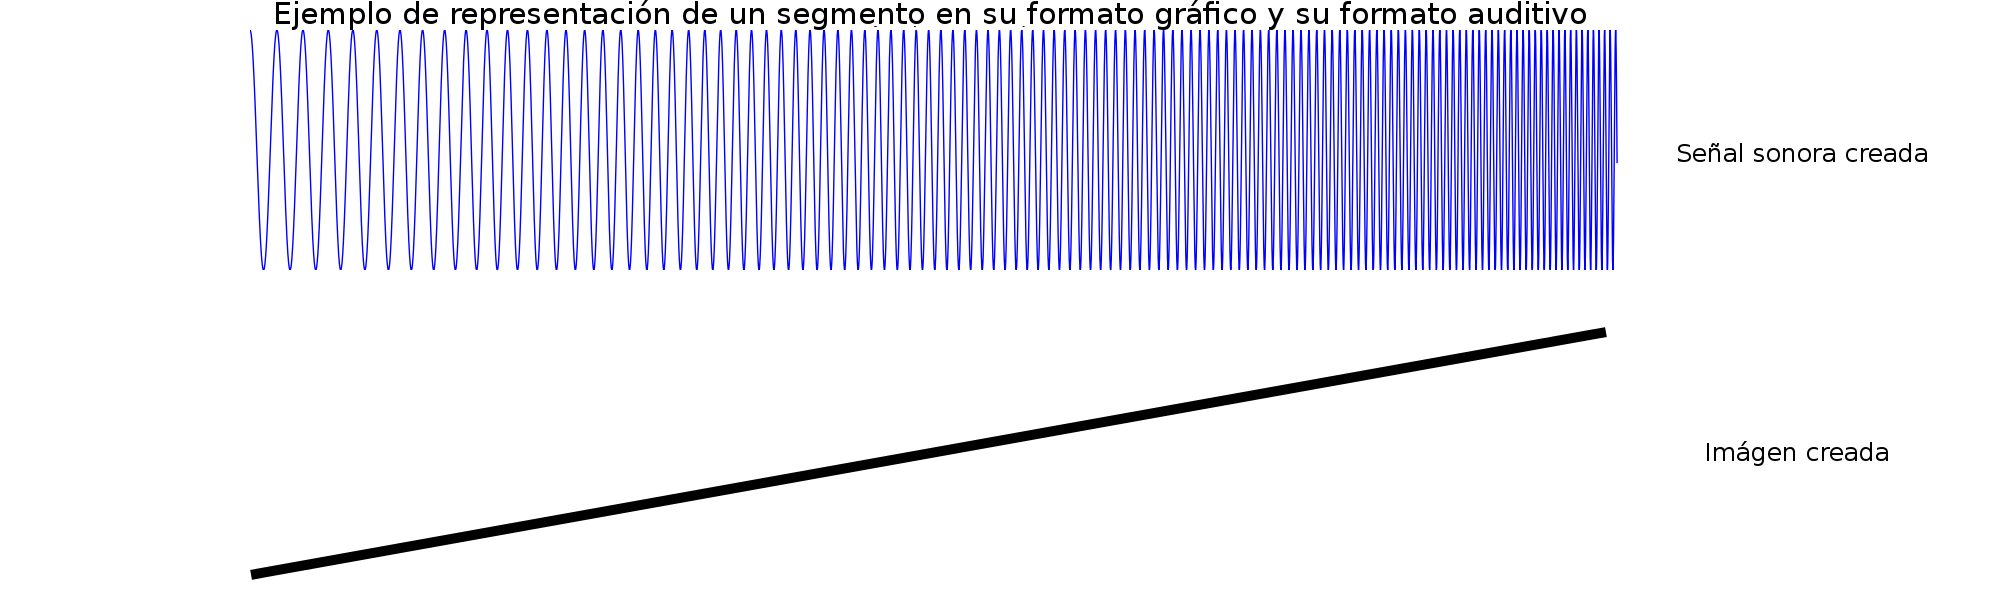
\includegraphics[width=\textwidth]{Imagenes/rampaFrec.png}
        \caption{Representación de un segmento en el espacio de frecuencias y tiempos y en el espacio geométrico tradicional. Se puede observar que a mayor altura corresponde una mayor frecuencias y que la variación en la representación sonora es continua y preservando las características conceptuales de la geometría deseada.}
        \label{fig:rampaFrec}
    \end{figure}
    
    Al implementar el código, e involucrar operaciones exponenciales surgió el problema de que numéricamente las computadoras no manejan fácilmente valores numéricos grandes \footnote{Los parámetros pueden ser ordenes de magnitud superiores a lo usual.} (por más que el resultado final fuera un números usual), por eso hubo que realizar las operaciones para calcular los parámetros de la representación utilizando una escala simbólica que fuera de 0 a 1 y luego reescalar los resultados obtenidos a la escala inicial. Realizando las cuentas se puede observar que partiendo de la relación \ref{ec:yToFrecInicial} se llega a las expresiones  \ref{ec:yToF1}, \ref{ec:yToF2} y \ref{ec:yToF3}. En la implementación numérica de estas soluciones siempre se uso como base b a la base decimal.
    
    \begin{equation}
        \label{ec:xTot}
        t = x \cdot \frac{T}{NroPixels}
    \end{equation}
    
    \begin{equation}
        \label{ec:yToFrecInicial}
        Frec(y) = A \cdot b^{y} + B
    \end{equation}
    
    con 
    
    \begin{equation*}
        Frec(Y_{max}) = A \cdot b^{y_{max}} + B
    \end{equation*}
    
    \begin{equation*}
        Frec(Y_{min}) = A \cdot b^{y_{min}} + B
    \end{equation*}
    
    donde se asume que $y_{min}=0$ por lo que que reescalando con Y* = Y/$Y_{max}$ queda que
    
    \begin{equation*}
        Frec(y*) = A \cdot b^{y*} + B
    \end{equation*}
    
    \begin{equation*}
        Frec(Y*_{max}) = A \cdot b^{1} + B
    \end{equation*}
    
    \begin{equation*}
        Frec(Y*_{min}) = A \cdot b^{0} + B
    \end{equation*}
    
    de donde sale que 
    
    \begin{equation}
        \label{ec:yToF1}
        A = \frac{Frec(Y_{max}) - Frec(Y_{min}) }{b^1-b^0}
    \end{equation}
    
    \begin{equation}
        \label{ec:yToF2}
        B = ((Frec(Y_{max}) + Frec(Y_{min})) - A \cdot (b^1 + b^0)) / 2
    \end{equation}
    
    \begin{equation}
        \label{ec:yToF3}
        Frec(Y) = A \cdot b^{Y/Y_{max}} + B
    \end{equation}
    
    \begin{figure}
        \center
        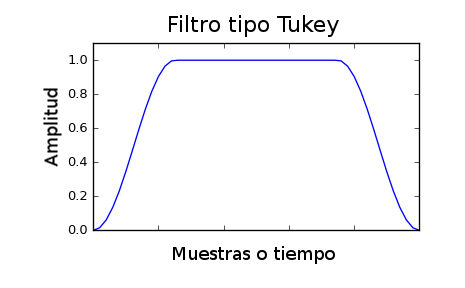
\includegraphics[width=0.5\textwidth]{Imagenes/tukey.png}
        \caption{Filtro que se le aplica a las rampas de sonido creadas para suavizar los extremos y que no aparezcan chasquidos (armónicos de alta frecuencia indeseados) en los extremos del mismo.}
        \label{fig:tukey}
    \end{figure}
    
    Una vez obtenidos los extremos en términos de frecuencia y tiempo para cada segmento, se debía crear con dichos parámetros una rampa de frecuencia, continua, que no tuviera los problemas de discretización inherentes a la pixelización de la imagen. Para eso se usó los código que se observa en \ref{code:rampa} donde a partir de los parámetros de cada segmento a transformar se crea la rampa de sonido.
    
    La base distintiva de esta función en relación al procedimiento usual del vOICe es que genera un continuo de frecuencias modificando la velocidad con que cambia la fase entre bit y bit en lugar de concatenar funciones armónicas de diferentes valores fijos de frecuencia. De esta manera se pueden crear saltos tan pequeños de fase como sean deseables sin que dichos saltos impliquen una discontinuidad en la onda generada \footnote{Hay un limite dado por el framerate del audio creado (en nuestro caso utilizamos una calidad de audio de 44100Hz), pero esta frecuencia de muestreo en el audio creado implica que se puede crear una rampa de frecuencia virtualmente continua}. 
    
    \spacing{1}
    \begin{minipage}{\textwidth}
    \begin{lstlisting}[caption=Código que genera una rampa de frecuencia que varia en forma continua. Cada una de estas rampas es la representación sonora equivalente a un segmento recto en la lógica del vOICe pero preservando la continuidad de la señal al cambiar en forma continua la frecuencia como se observa en la figura \ref{fig:rampaFrec}., label=code:rampa]
    
    /**
	 * Create a sound that change in frecuencie in logaritmic form
	 * 
	 * 
	 * @param freci
	 *            Inicial value of frecuence
	 * @param frecf
	 *            Final value of frecuence
	 * @param ti
	 *            Time (in sec) initial
	 * @param tf
	 *            Time (in sec) final
	 * @return
	 * 
	 */
	private double[] createMusicRamp(double freci, double frecf, double ti, double tf) {
		double dt = 1 / (double) fs; // es el dt que transcurre entre sample y sample
		long N = Math.round((tf - ti) * fs); // El numero de samples que hay que crear
		double[] frec = logspacelog(freci, frecf, N, base); // Crea una escala logaritmica en base 10 que va de la frecuencia inicial a la final
		for (int i = 0; i < frec.length; i++) { // Lo multiplica x 2pi para trabajar con la fase
			frec[i] = frec[i] * 2 * Math.PI;
		}
		// Integra las freciencias instantaneas
		for (int i = 1; i < frec.length; i++) {
			frec[i] = frec[i - 1] + frec[i] * dt; // El primero lo deja tal cual y despues suma hasta el ultimo
		}
		// ahora frec es la fase instante a instante

		// Vamos a hacer el coseno de la fase
		for (int i = 0; i < frec.length; i++) {
			frec[i] = Math.cos(frec[i]);
		}
		// Ya esta creado el sonido

		frec = tukeywin(frec, 0.02);

		return frec;

	}
	\end{lstlisting}
    \end{minipage}

    \spacing{1.5}
	
	\spacing{1}
	\begin{minipage}{\textwidth}
    \begin{lstlisting}[caption=Código que aplica el filtro tipo Tukey (ver figura \ref{fig:tukey}) para evitar la inclusión de armónicos por el efecto de los contornos., label=code:tukey]
     /**
	 * Aplica una funcion tipo tukeywin (que suaviza los extremos)
	 * 
	 * @param frec
	 *            Es el array de datos de entrada
	 * @param d
	 *            es el parametro de cuanto suavizar. Si es un numero menor que uno asume que es el porcentaje (por unidad), si es mayor que es numero de frames
	 *            a suavizar
	 * @return Devuelve el input suavizado
	 */
	private double[] tukeywin(double[] frec, double d) {
		int framesMaximos;

		if (d >= 1) { // recupera cuantos frames tiene que suavizar
			framesMaximos = (int) d;
		} else {
			framesMaximos = (int) (frec.length * d);
		}

		if (framesMaximos != 0) {

			// suaviza los frames del inicio
			for (int i = 0; i < framesMaximos; i++) {
				double fase = (double) i / framesMaximos * Math.PI;
				double factor = (-Math.cos(fase) + 1) / 2;
				frec[i] = frec[i] * factor;
			}

			// suaviza los frames del final
			for (int i = 0; i < framesMaximos; i++) {
				double fase = (double) i / framesMaximos * Math.PI;
				double factor = (-Math.cos(fase) + 1) / 2;
				frec[frec.length - 1 - i] = frec[frec.length - 1 - i] * factor;
			}
		}
		return frec;
	}
	\end{lstlisting}
	\end{minipage}
    \spacing{1.5}
    
    Un procesamiento diferente de los datos requirió la construcción de los segmentos verticales, ya que estos conceptualmente no representan una variación de la frecuencia en función del tiempo sino un conjunto simultaneo de frecuencias. Para resolver este problema se consideró la creación de un pulso limitado en frecuencias, sin embargo esto trajo problemas, ya que por un lado dichos pulsos (sobre todo al incluir frecuencias bajas) eran largos en el tiempo y sonaban apreciablemente antes y después del momento en que se encontraba el segmento vertical. Por otro lado, más allá de la cuestión de la duración temporal, tenían una conformación perceptualmente diferente a la de una rampa, por lo que era fácil distinguirlos del resto de los estímulos. Como parte de los objetivos era observar la dependencia de la capacidad de percibir frente a transformaciones de rotación, distinguir constructivamente estos estímulos en forma no continua respecto a los parámetros de rotación no era una buena idea. 
    
    Para solucionar este problema, se eligió una pendiente mínima que pareciera a priori suficientemente inclinada como para que no se pudiera distinguir un estimulo ascendente de uno descendente, y se forzó a los segmentos verticales a tener esta pendiente mínima. En base a pruebas preliminares se eligió una diferencia temporal entre inicio y fin de los segmentos de 0.01 segundos (distancia que además en términos de la representación visual tampoco era distinguible), de esta manera todos los segmentos se construyeron con la misma lógica y algoritmo. En pruebas posteriores cuantitativas pudimos ratificar que el límite estimado estaba por debajo de la capacidad de percepción de los sujetos. 
    
    \begin{figure}
        \center
        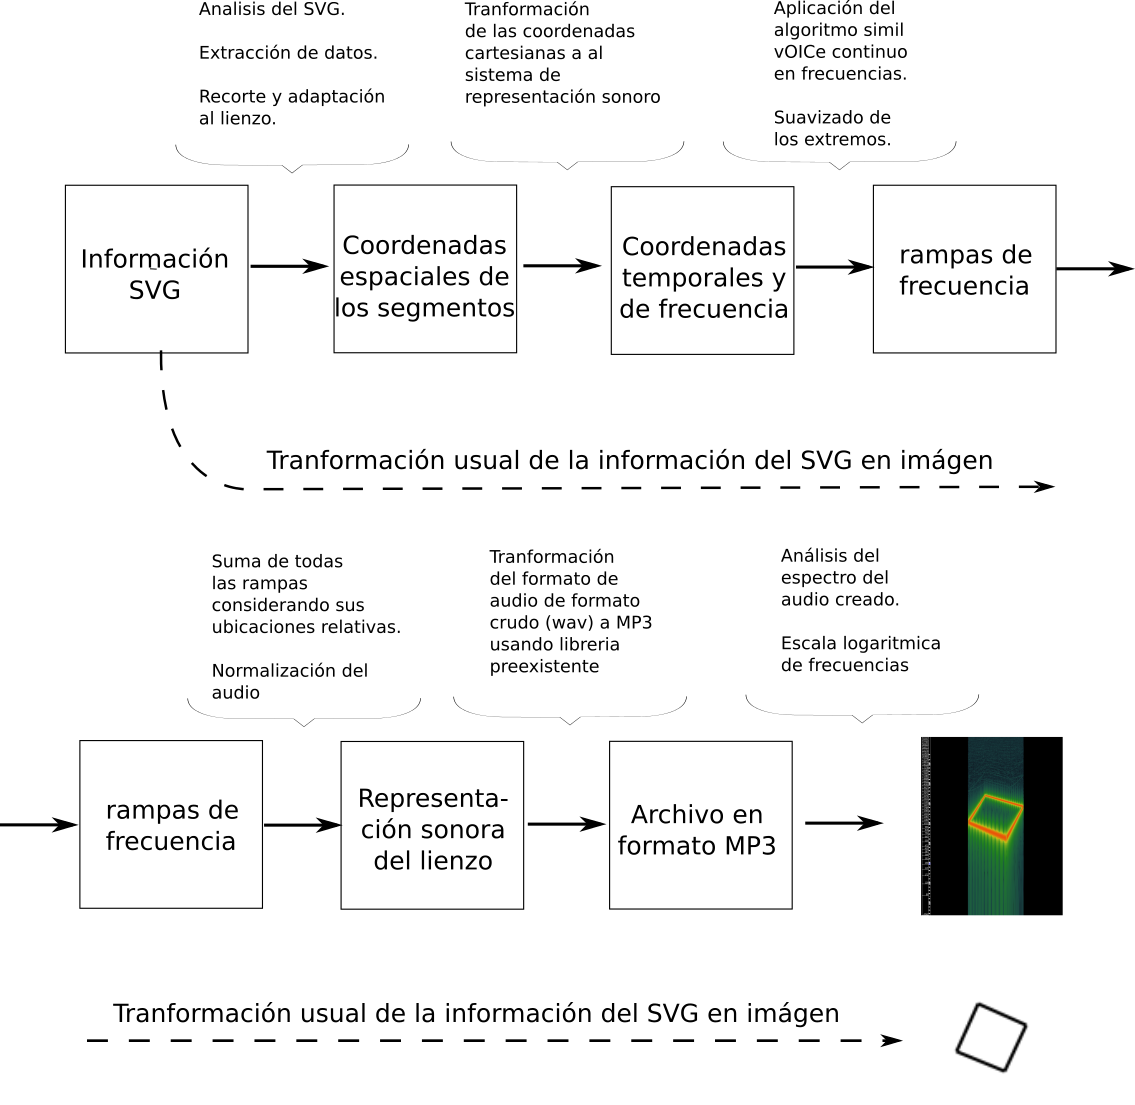
\includegraphics[width=\textwidth]{Imagenes/diagramaSVG2.png}
        \caption{Resumen del procesamiento realizado para transformar la información conceptual de las figuras almacenado en formato vectorial (SVG) a su representación sonora siguiendo una lógica equivalente al vOICe pero que preserve características geométricas.}
        \label{fig:diagramaSVG}
    \end{figure}
    
    Una vez generadas todas las rampas de sonido correspondientes a todos los segmentos se les aplicó un filtro tipo Tukeywin \footnote{para evitar los chasquidos correspondientes al inicio y el fin de cada segmento} (detallado en el código \ref{code:tukey} y ejemplificado en la figura\ref{fig:tukey}) y luego se las sumó (correctamente ubicadas en el tiempo) y normalizó para generar una única secuencia por imagen que la librería correspondiente pueda transformar en un archivo de audio WAV. Una vez creado el WAV por una cuestión del volumen de datos utilizados (para realizar cada experimento se requieren miles de estímulos similares) se transformó los archivo WAV en MP3. 

    \begin{figure}
        \center
        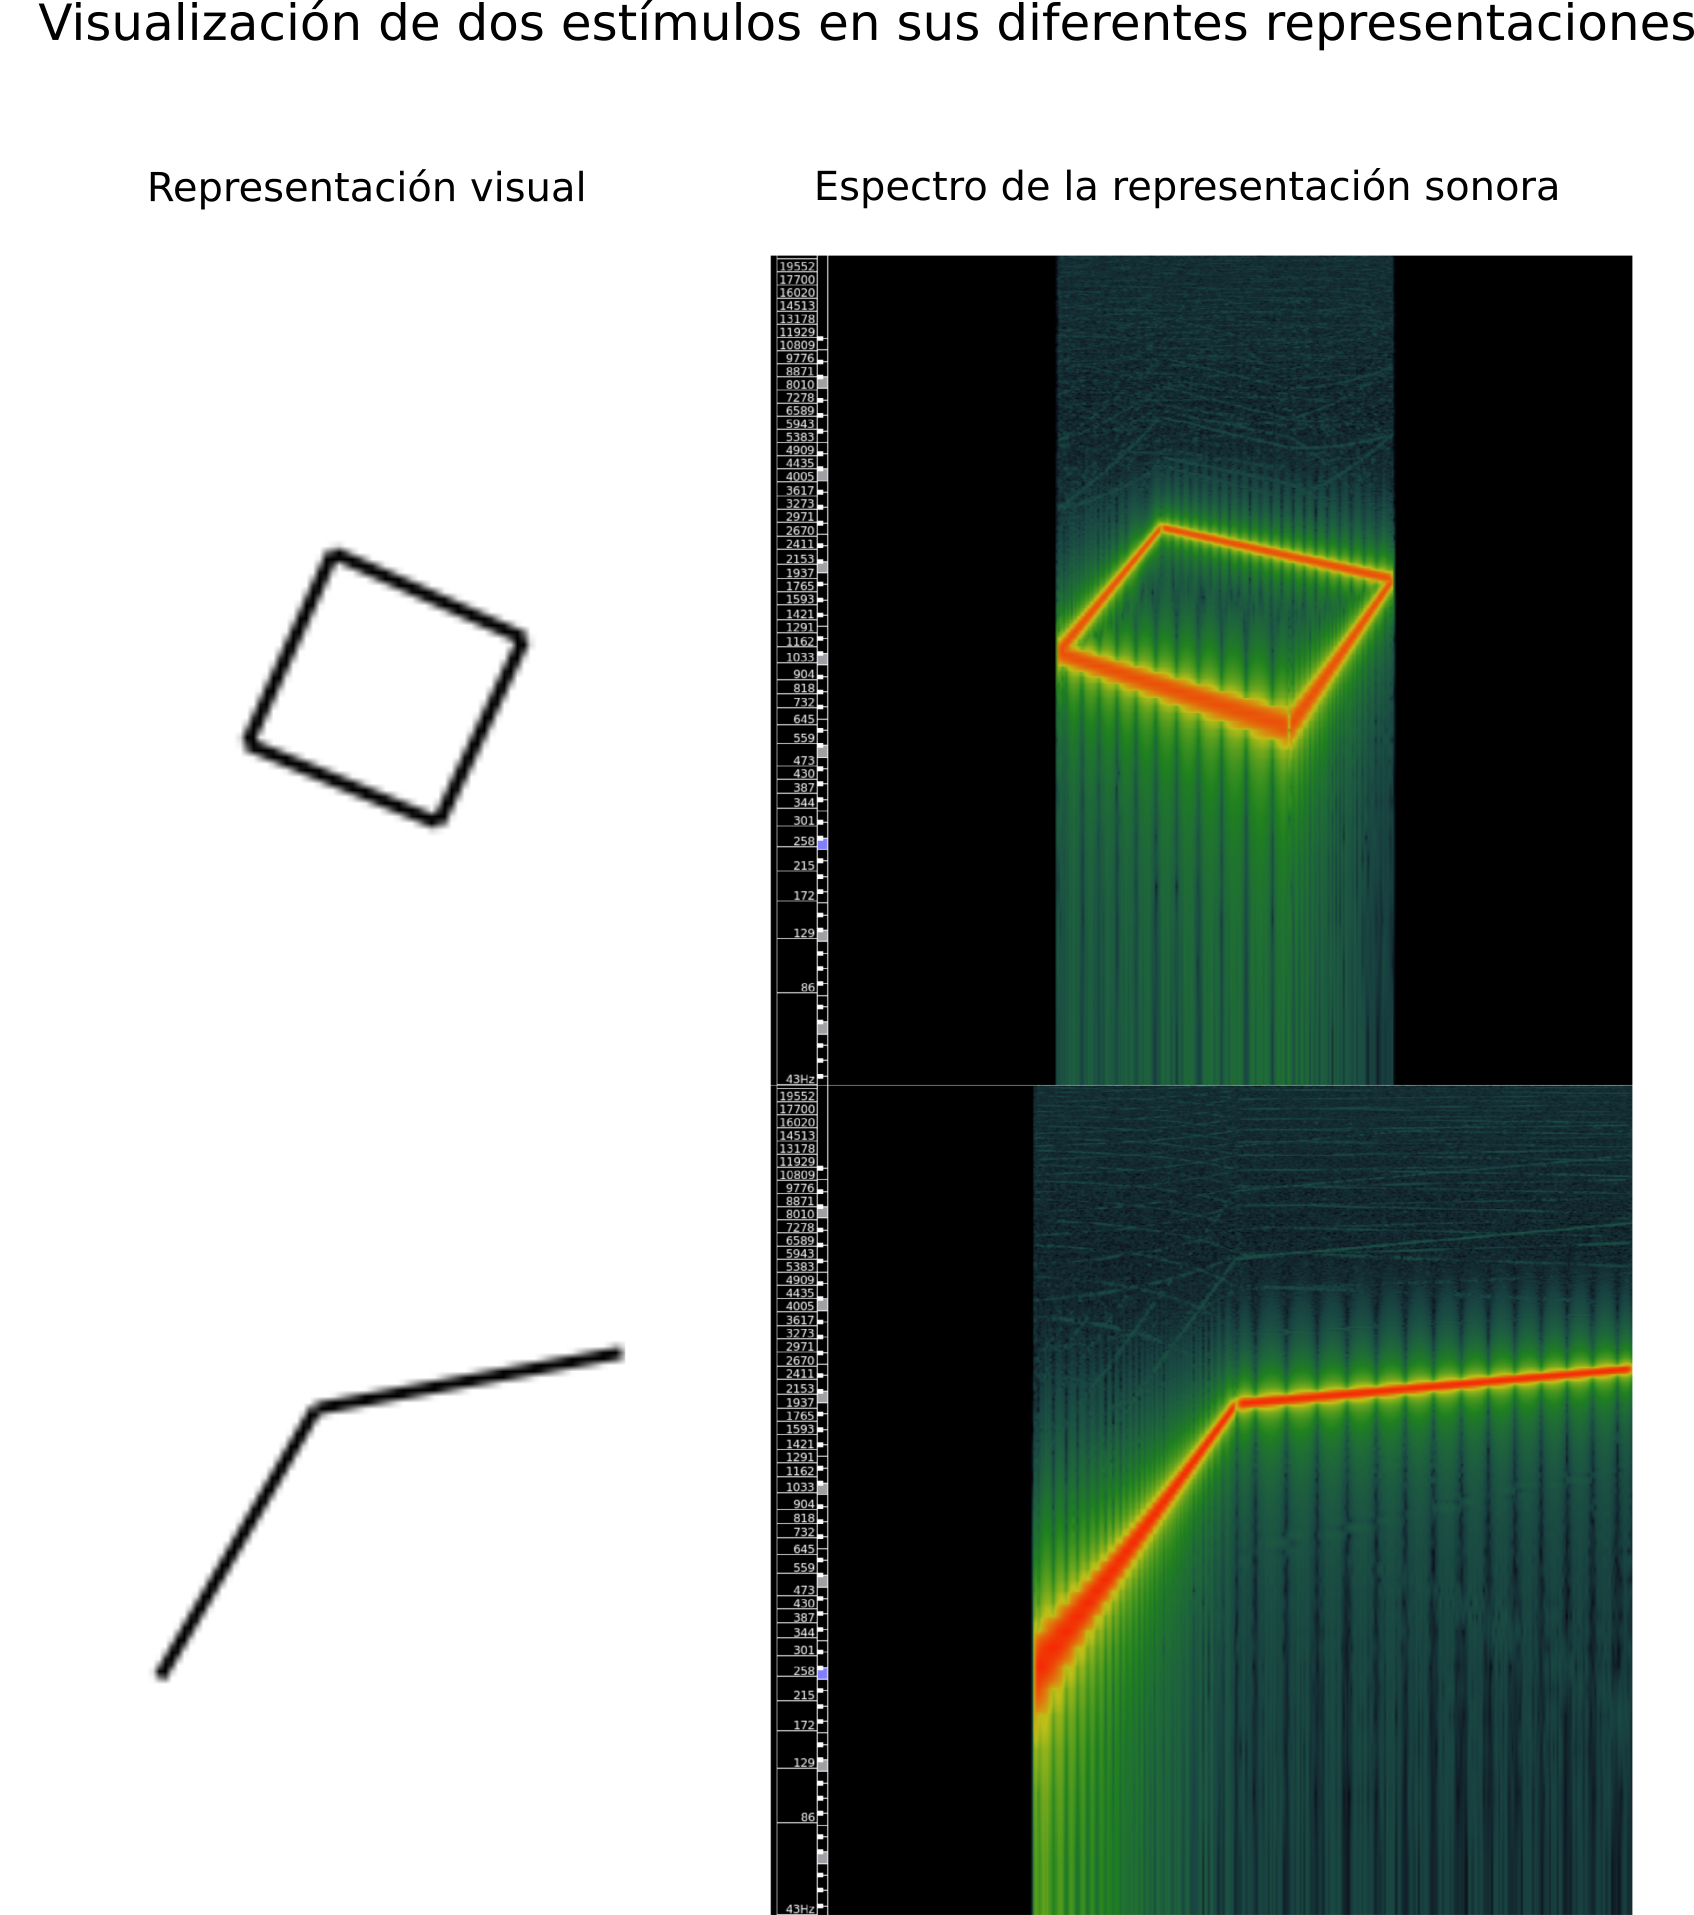
\includegraphics[width=\textwidth]{Imagenes/TranformacionSVG.png}
        \caption{Ejemplos del proceso de comparación de imágenes representadas en su formato gráfico y su correspondiente espectro en función del tiempo (en escala logarítmica), donde se observa la preservación de la forma en la transformación de representaciones. Notar que el aparente efecto de profundidad es debido al arbitrario de las escalas de representación, que no es exactamente igual en ambas figuras.}
        \label{fig:TransformacionSVG}
    \end{figure}

    
\subsection{Desarrollo del software utilizado}

    La creación, escritura y diseño de la plataforma con el que se realizaron todas las mediciones fue el aspecto que más tiempo demando a lo largo todo el trabajo. Para realizar las pruebas era necesario contar con alguna plataforma que permitiera realizar los test propuestos, y dado que se desconocía en un inicio como serían los resultados preliminares se intento no limitar con la herramienta las posibilidades futuras. Es importante remarcar que si bien el desarrollo de la plataforma en si nunca fue el objetivo de este trabajo, si sirvió como aprendizaje para adquirir un enorme cantidad de conocimiento y experiencia en la tarea de programar y desarrollar un proyecto de cierta complejidad. 
    
    La entorno elegido para escribir el código fue LibGDX (\url{https://libgdx.badlogicgames.com/}), una variante de JAVA pensada mas que nada para programar videojuegos que posee la ventaja de disponer de todas las funcionalidad usuales de JAVA para generar interfaces gráficas en forma sencilla, con el agregado de que permite compilar la aplicación resultante en JAVA para JavaVirtualMachine (Pcs), para Java para Android, para iOS (Mac) y para HTML5 (JavaScript). 
    
    Con esta plataforma y todas estas opciones de las que disponía, se esperab eventualmente poder diseñar o bien una versión de la plataforma apta para realizar experimentos controlados en laboratorio, o bien una plataforma que tomara mediciones en forma solapada detrás de algún tipo de desafío que se pudiera realizar en forma más masiva a través de celulares o una página web. 
    
    Sin embargo tras observar los resultados preliminares, y encausar el diseño experimental a un protocolo con sesiones de larga duración, resultó cada vez más evidente que no tenia sentido realizar mediciones fuera del laboratorio, por lo que terminamos usando la plataforma simplemente como una aplicación en PC que se adaptara a las necesidades de los sucesivos diseños experimentales. 
    
    Para poder realizar los experimentos (más allá de los detalles de cada configuración experimental en particular) necesitábamos una aplicación que tuviera las siguientes funcionalidades:
    
    \begin{itemize}
        \item Fuera capaz de mostrar estímulos, ya sea visuales, o sonoros
        \item Fuera capaz de recibir como respuesta la selección de alguna opción entre varias.
        \item Fuera capaz de manejar una lógica de niveles y trials secuenciales
        \item Fuera capaz de registrar y almacenar toda la información relevante para poder reproducir lo que el usuario o sujeto experimental realizara. 
    \end{itemize}
    
    Para realizar estas tareas se pensó en una estructura de programación orientada a objetos donde cada usuario tuviera que realizar niveles, cada nivel estuviera conformado por un conjunto de pruebas (o Trials), y cada Trial consistiera en un conjunto de cajas seleccionables con estímulos dentro. 
    
    Para crear la aplicación y que se ejecutara el experimento, era necesario previamente haber generado el contenido: niveles, Trials y estímulos. Por eso, la aplicación tuvo dos desarrollos paralelos, por un lado el código que se usara en tiempo de ejecución de los experimentos, que debía manipular toda la información relevante, y por otro lado un código que generara instancias de los objetos a usar, es decir un generador de niveles, Trials y estímulos compatibles con el resto del código.
    
    El desarrollo del software (al que apodamos Visound) estuvo muy ligado a los cambios de diseño experimental que se fueron realizando a lo largo del tiempo. Pese a que cualquier análisis del mismo en un momento dado implica ignorar las funcionalidades especificas que se fueron modificando hubo un proceso acumulativo a lo largo del tiempo. Para dar una noción del trabajo realizado se describirá por una parte estadísticas de la evolución temporal del proyecto y por otro breve detalle del código con que se realizó el último experimento. 
    
    \subsubsection{Evolución y estadísticas del código de la plataforma con que se realizó los experimentos}
    
    \begin{figure}
        \center
        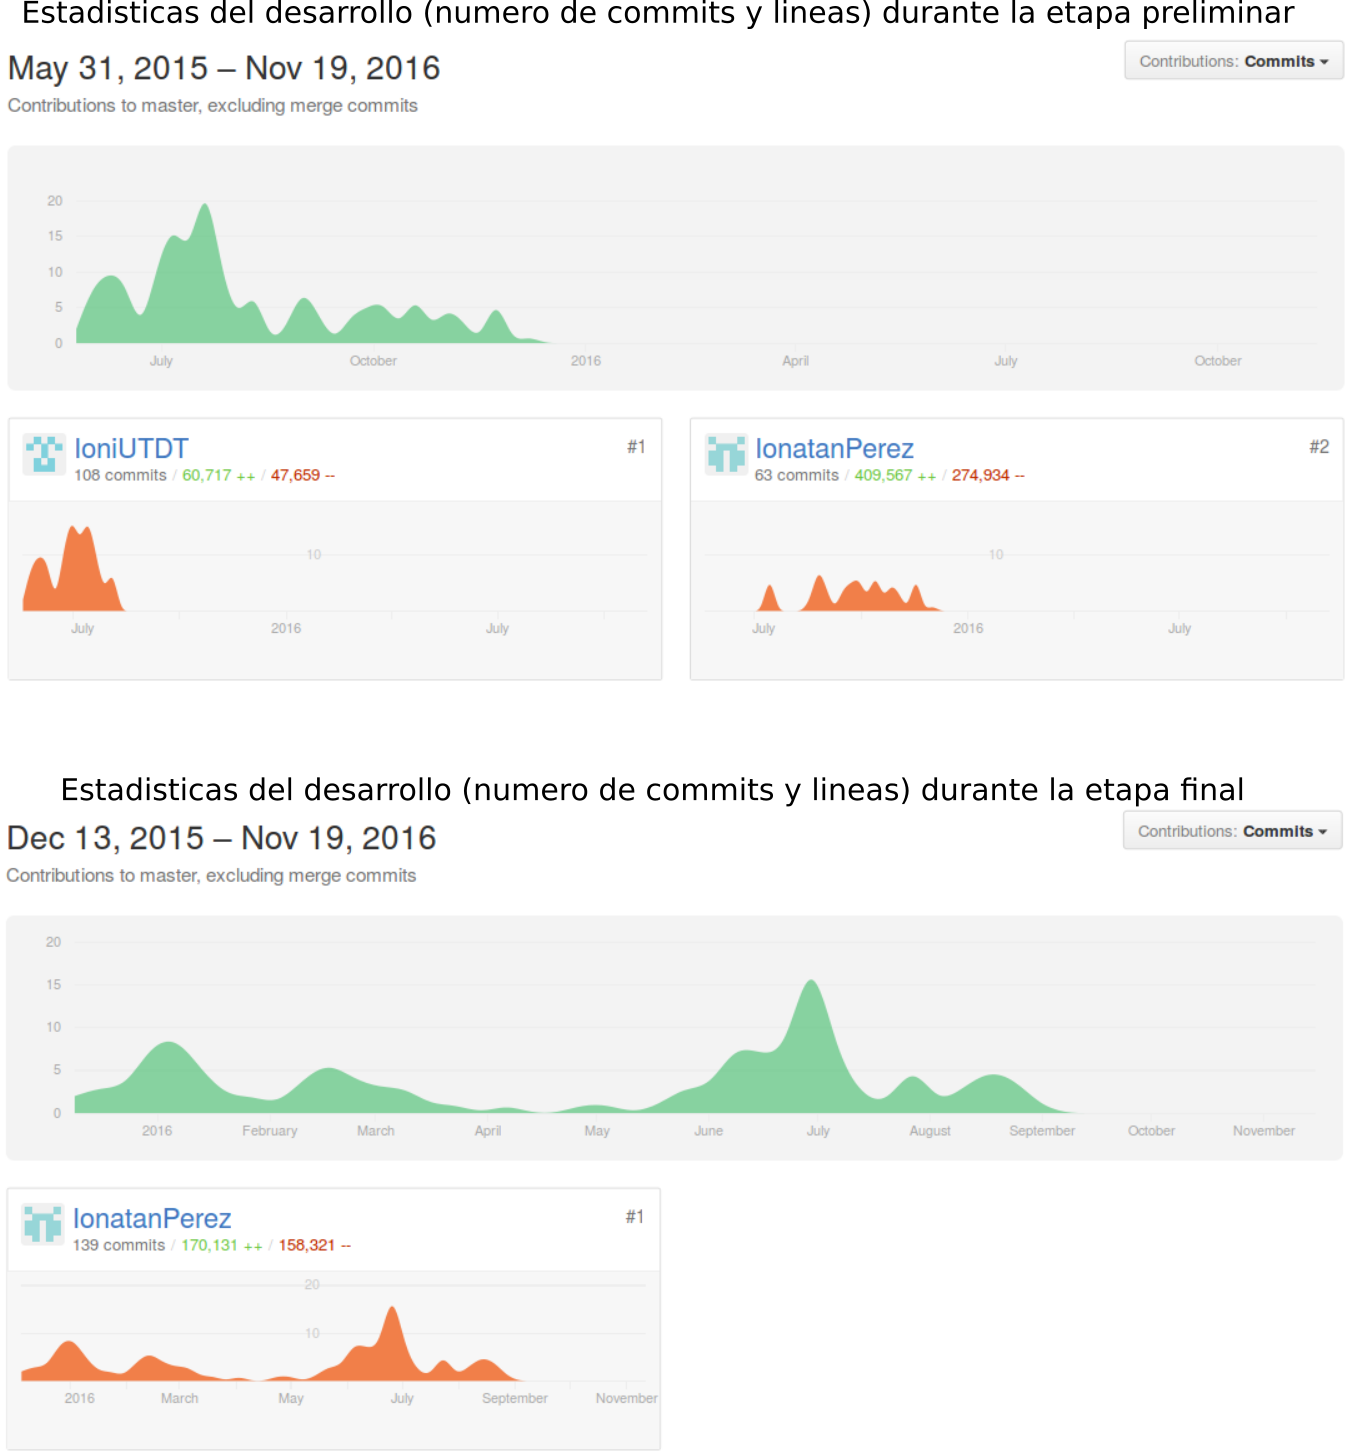
\includegraphics[width=\textwidth]{Imagenes/Commits.png}
        \caption{Estadísticas de la evolución del proyecto a lo largo de sus dos etapas, la preliminar que incluyo las pruebas conceptuales y las calibraciones preliminares y la etapa final en la cual se estuvieron realizando mediciones. Se observa junto a los commits realizados el numero de lineas agregadas y quitadas, sin embargo dicho numero incluye las lineas dentro de los archivos correspondientes a los estímulos y la información de niveles y trials. En la figura \ref{fig:Lineas} se observa un detalle de dicha información}
        \label{fig:Commits}
    \end{figure}
    
    \begin{figure}
        \center
        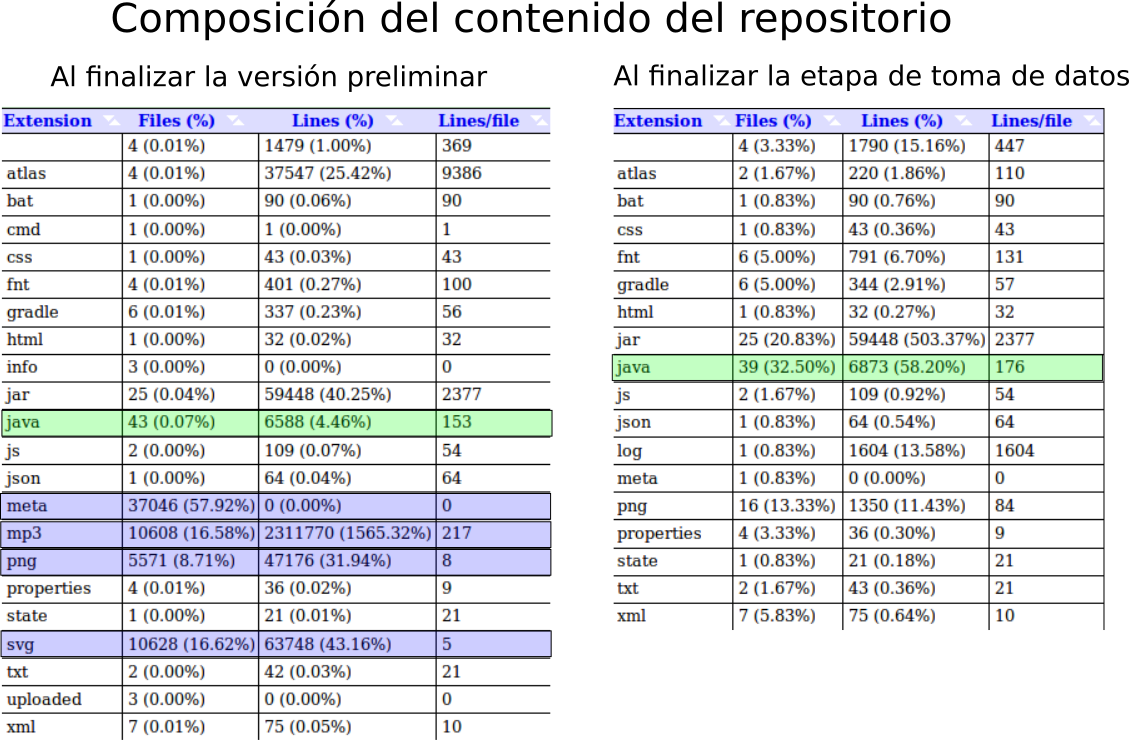
\includegraphics[width=\textwidth]{Imagenes/Lineas.png}
        \caption{Estadísticas del contenido del repositorio online donde guardamos el control de versiones del proyecto comparando entre la finalización de la etapa de desarrollo preliminar y la última versión del proyecto. Se observar que en un principio la mayor parte de las lineas corresponden a material relacionado a los estímulos y los niveles (archivos mp3, SVG, meta, png). En la etapa final excluimos dichos archivos del control de versiones porque eran generados por el propio código. Se puede observar que entre la versión preliminar y la final la cantidad de lineas de los archivos JAVA donde se encuentra el núcleo del trabajo no se incrementa mucho, sin embargo entre ambos momentos hubo un completo y profundo proceso de reescritura para adaptar el código a una concepción mucho mas abstracta, y genérica de funcionamiento que permitiera cambiar los experimentos modificando unos pocos parámetros.}
        \label{fig:Lineas}
    \end{figure}
        
    Desde un momento temprano del desarrollo del códigos decidimos utilizar un control de versiones. Elegimos usar Git, y sincronizar el contenido del Git con el servidor de repositorios online GitHub. En cierto momento, cuando la aplicación ya estaba en estado de desarrollo funcional, creamos un repositorio nuevo, por lo que todas los registros presentan una discontinuidad en ese punto. Las versiones preliminares del código se encuentran alojadas en \url{https://github.com/IoniUTDT/contornos}, mientras que las versiones posteriores con las que se hicieron todas las mediciones experimentales se encuentran en \url{https://github.com/IoniUTDT/VisoundJavaCode}. En dichos repositorios figuran estadísticas automáticas acerca del contenido de los proyectos y su nivel de actividad. También para algunas mediciones reportadas utilizamos el software Gitstats.
    
    Como se puede ver en la figura \ref{fig:Commits}, el conjunto de los dos repositorios contó con 312 commits\footnote{Un commit es un punto del tiempo en el que se crea un control para comparar pasados y futuros cambios} (173 en el código inicial entre mayo del 2015 y diciembre de 2016 y 139 la versión final entre diciembre de 2016 y septiembre de 2016 en que se concluyó con el desarrollo de la ultima versión utilizada). En los repositorios se observa una gran cantidad de lineas, sin embargo es importante destacar que no todas las lineas son de código escrito a mano, ya que la mayor parte del contenido del proyecto se genera en forma automática. En un principio el control de versiones incluía una revisión de todo el contenido. A medida que los estímulos utilizados se fueron construyendo en forma más masiva y automatizada cada vez era mayor la cantidad de archivos cuyo registro se volvió innecesario, por lo que en la etapa final los excluimos del control de versiones. 
    
    Por otro lado como se puede ver en el detalle del contenido de los repositorios (ver figura \ref{fig:Lineas}) la cantidad de lineas incluidas en los archivos JAVA (donde esta el código escrito a mano del proyecto) no varió significativamente entre el final de la etapa de preliminar y la última versión del experimento. Sin embargo la cantidad de lineas no es necesariamente una medida de calidad, ni de trabajo, ya que durante todo el proceso de escritura el código fue revisado y fueron reelaboradas la estructura de las clases, los objetos y la lógica de funcionamiento para hacer cada vez mas abstracto y flexible el código. En general el desarrollo de cada funcionalidad consistió en una primera versión de prueba y puesta a punto con alguna implementación especifica y una posterior reescritura para parametrizar e integrarlo al código general de forma que lo pensado pudiera adaptarse a diferentes implementaciones correspondientes a diferentes diseños experimentales. 
    
    \subsubsection{Estructuras y especificaciones de la plataforma desarrollada.}
    
    \begin{figure}
        \center
        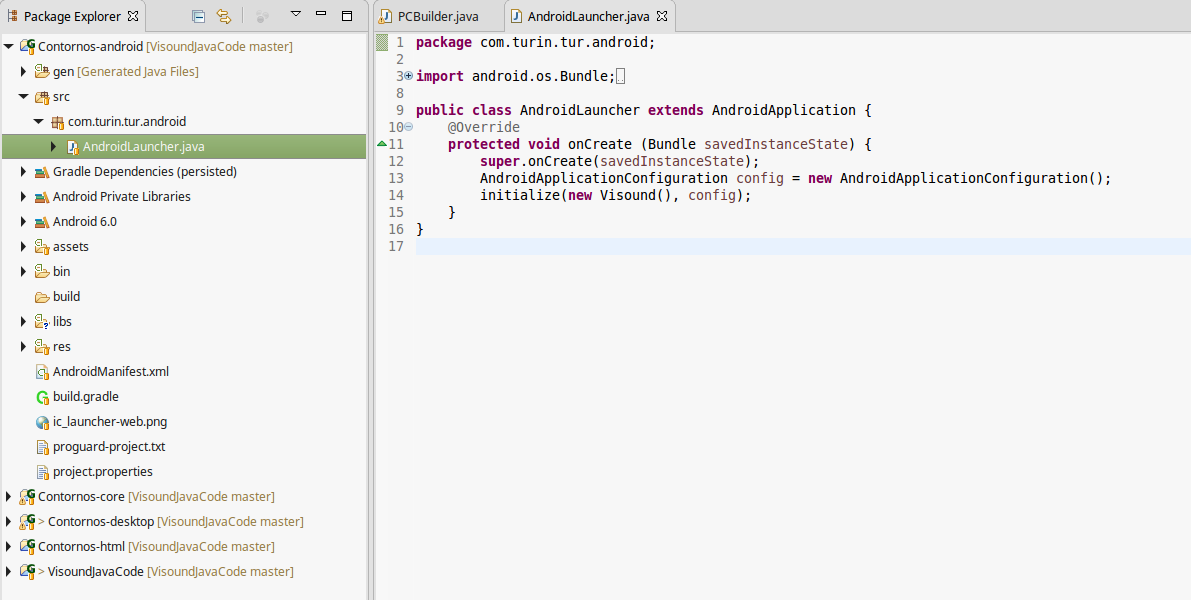
\includegraphics[width=\textwidth]{Imagenes/Eclipse1.png}
        \caption{Estructura general de la aplicación (cuyo nombre original fue 'Contornos' y luego 'Visound') visualizada en el entorno de programación Eclipse. Se observa que cada plataforma (sistema operativo) posee su propia estructura de archivos de configuración y clases que se encargan lanzar la aplicación desarrollada adecuadamente según el dispositivo destino. En nuestro caso configuramos el proyecto inicialmente para que se pudiera ejecutar en Java (desktop), en Android y en HTML. En la carpeta Core se encuentra todo el código de la aplicación (cuya clase principal se llama Visound) y que es independiente de la plataforma a la que se lo compile.}
        \label{fig:Eclipse1}
    \end{figure}
    
    \begin{figure}
        \center
        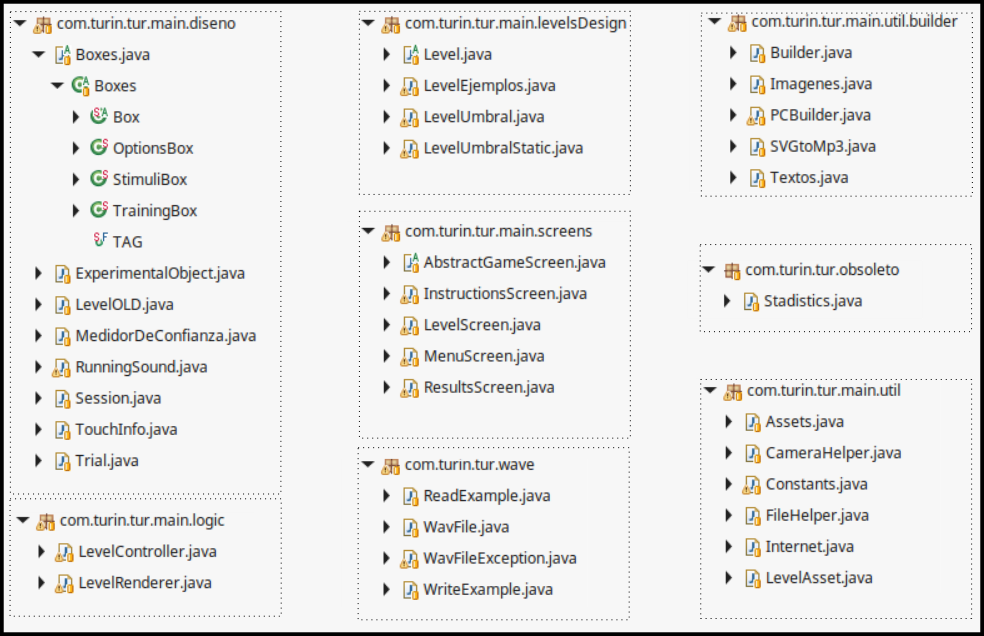
\includegraphics[width=\textwidth]{Imagenes/Clases.png}
        \caption{Estructura de clases de la aplicación en su última versión. Algunas clases como Boxes o Levels son clases abstractas que sirven para asegurar que todas las clases que implementen a las cajas con estímulos o los diferentes niveles cuenten con funcionalidad básicas que hacen al esquema general de funcionamiento del programa. Un breve detalle de la funcionalidad de cada clase se puede consultar en el anexo \ref{anexo:Clases}}
        \label{fig:Clases}
    \end{figure}
    
    \begin{figure}
        \center
        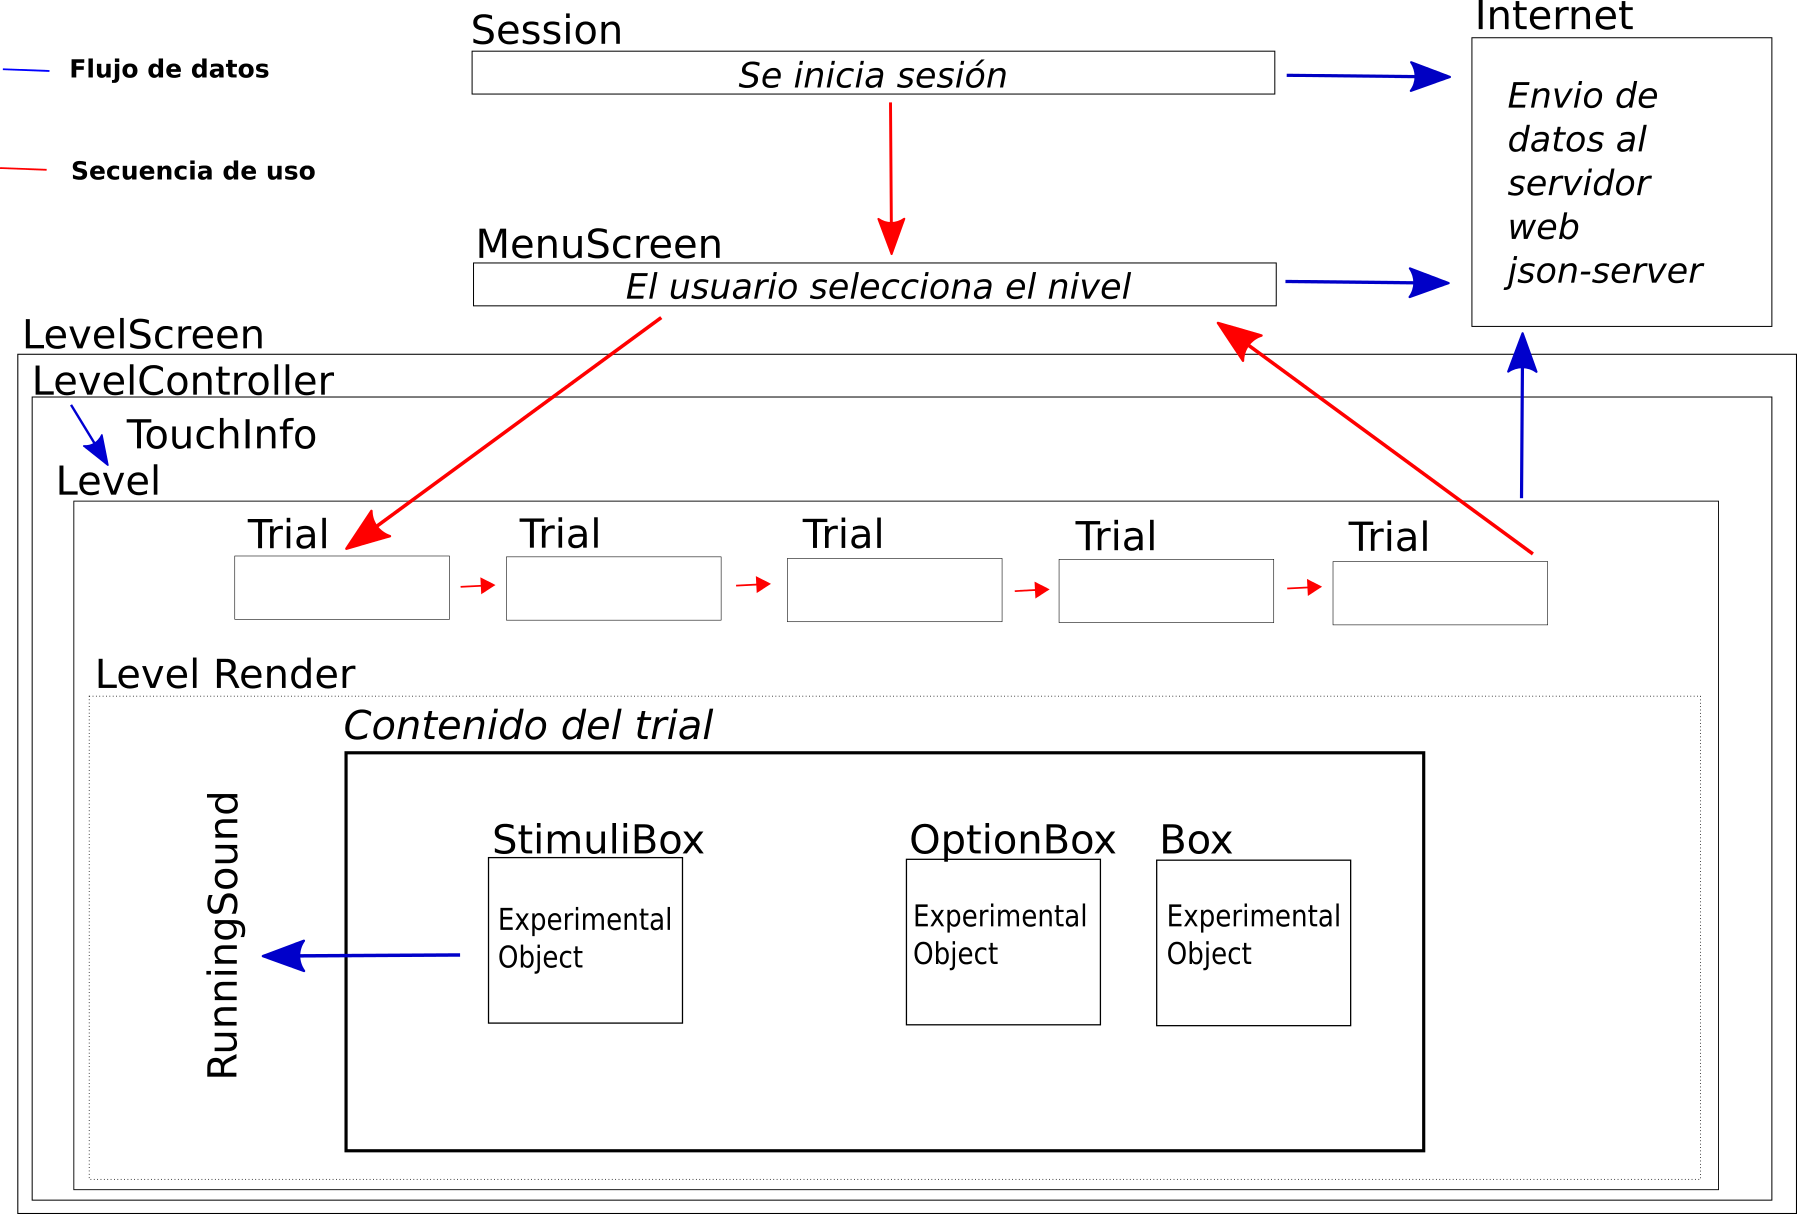
\includegraphics[width=\textwidth]{Imagenes/FlujoJava.png}
        \caption{Diagrama general de la aplicación, sus clases y la dinámica de su funcionamiento donde se explicitan los flujos de información entre clases. Los envíos de datos a internet se separan entre registros de sesión, registro de inicio de niveles (que incluye datos contextuales de lo que ya hizo el usuario), y el registro de las respuestas de los Trials que se realiza al concluir cada nivel. Un detalle de las clases y sus funciones de puede consultar en el anexo\ref{anexo:Clases}}
        \label{fig:Flujo}
    \end{figure}

        
    Como se menciono anteriormente la aplicación fue desarrollada en el framework LibGDX, y para su desarrollo se utilizo el IDE (Entorno gráfico de programación) Eclipse que posee diversas herramientas para desarrollar, ejecutar, testar y analizar el código. Eclipse es una plataforma abierta (\url{https://eclipse.org/}) que permite a la comunidad de desarrolladores generar herramientas de libre disponibilidad en internet para que cada usuario puede adaptar el entorno a sus necesidades. Como LibGDX es un framework orientado a multiplataforma, parte de la configuración del entorno de trabajo incluye el uso de paquetes y herramientas (de instalación automática) que permitan la correcta interacción de la aplicación desarrollada con los entornos y las librerías de JAVA y de Android. Parte de las herramientas utilizadas incluyeron simuladores de sistemas operativos android virtuales y herramientas de debug especificas para hacer pruebas en celulares además de las típicas disponibilidades para testar el código en PCs
    
    Como se puede ver en la figura \ref{fig:Eclipse1}, la estructura que utiliza LibGDX para crear sus aplicaciones se basa en separar la aplicación en si misma por un lado (encapsulado en un paquete denominado Core) y una serie de empaquetados específicos donde se genera y configura (en forma automática aunque se puede modificar) los aspectos que hacen a la ejecución en las diferentes plataformas. Al compilar la aplicación, según para que plataforma se la compile, ejecuta primero el código especifico de la plataforma (la clase Launcher correspondiente a cada sistema operativo), y luego esta clase inicializa la aplicación que uno haya desarrollado. De esta manera se puede independizar el desarrollo conceptual de la aplicación de los detalles específicos que hacen a la interacción con cada plataforma. 
    
    En la figura \ref{fig:Clases} se puede observar un resumen de toda las clases que conforman a la aplicación en su última versión. Una breve descripción de cada una de ellas se puede consultar en el anexo \ref{anexo:Clases}. En la figura \ref{fig:Flujo} se puede observar el funcionamiento típico de las principales clases y como se anidan e interrelacionan. 
    
            
    \begin{figure}
        \center
        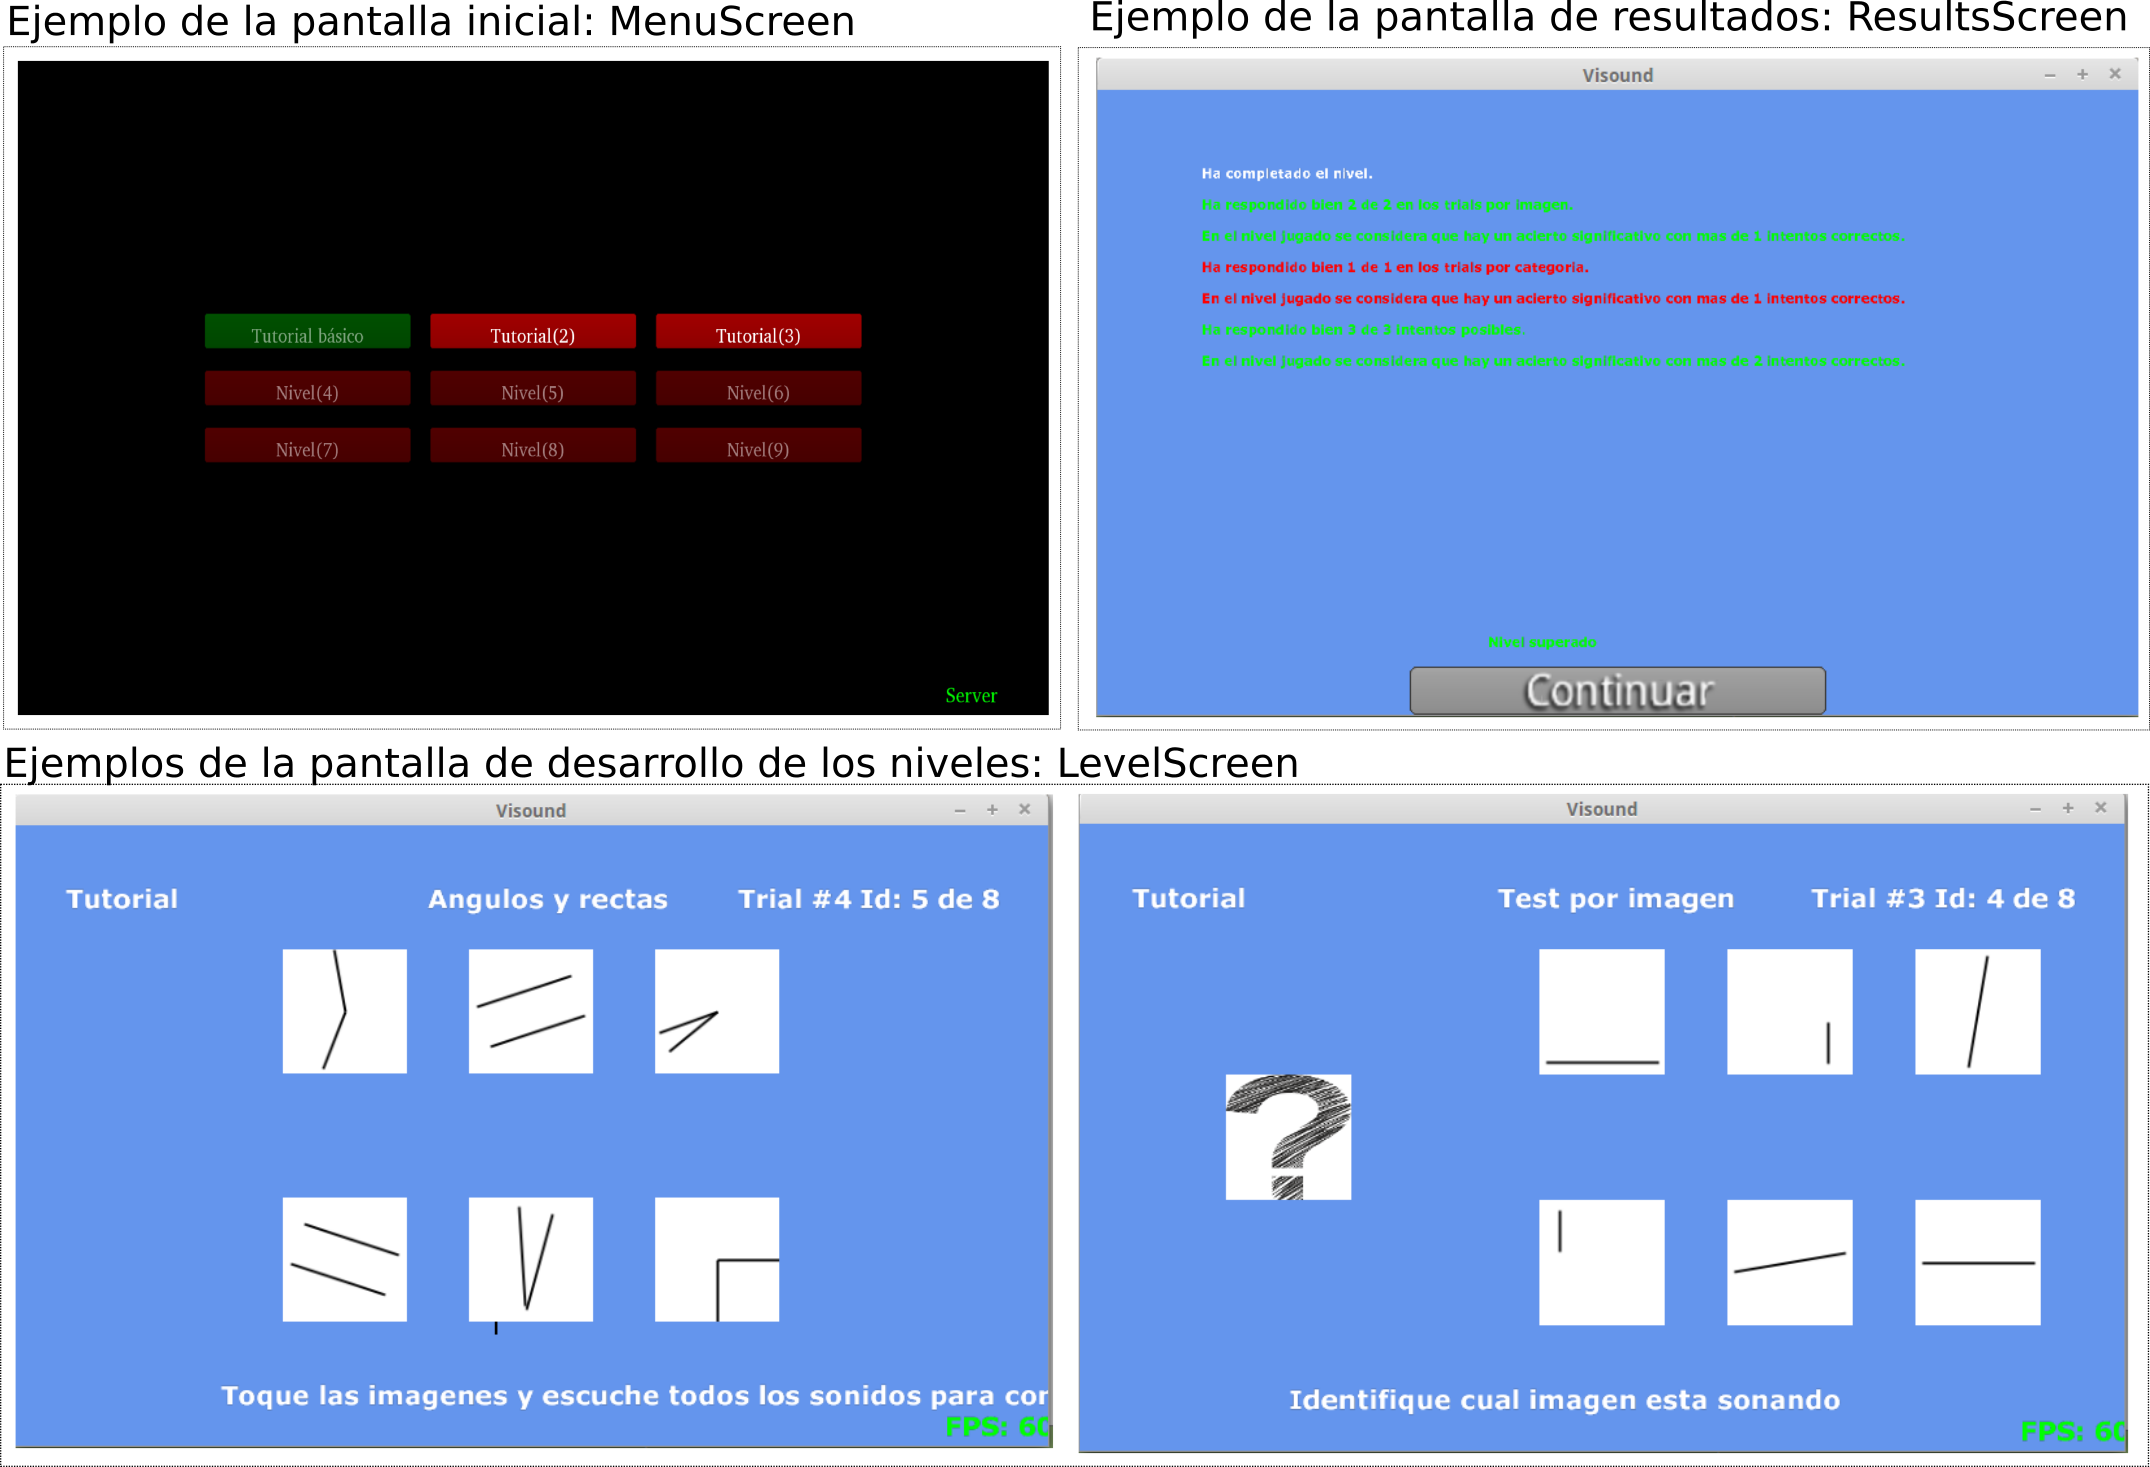
\includegraphics[width=\textwidth]{Imagenes/Pantallas1.png}
        \caption{Ejemplos de  capturas de pantalla de la aplicación en etapas tempranas de desarrollo. Arriba a la izquierda se observa el menú principal de la aplicación, en una versión del experimento donde ya se había implementado la habilitación secuencial de niveles. A su derecha se observa la pantalla de resultados ideada como un reporte al usuario en una versión temprana del desarrollo, luego esta opción se discontinuó. Abajo a la izquierda se observa una pantalla de tutorial donde se puede seleccionar las imágenes para escuchar su correspondiente sonido, y a su derecha se observa una pantalla tipo test donde el sujeto debe identificar entre las figuras cual es la que esta sonando. Ambas imágenes además muestran información de dubug porque corresponden a etapas de desarrollo. }
        \label{fig:Pantallas1}
    \end{figure}
    
    \begin{figure}
        \center
        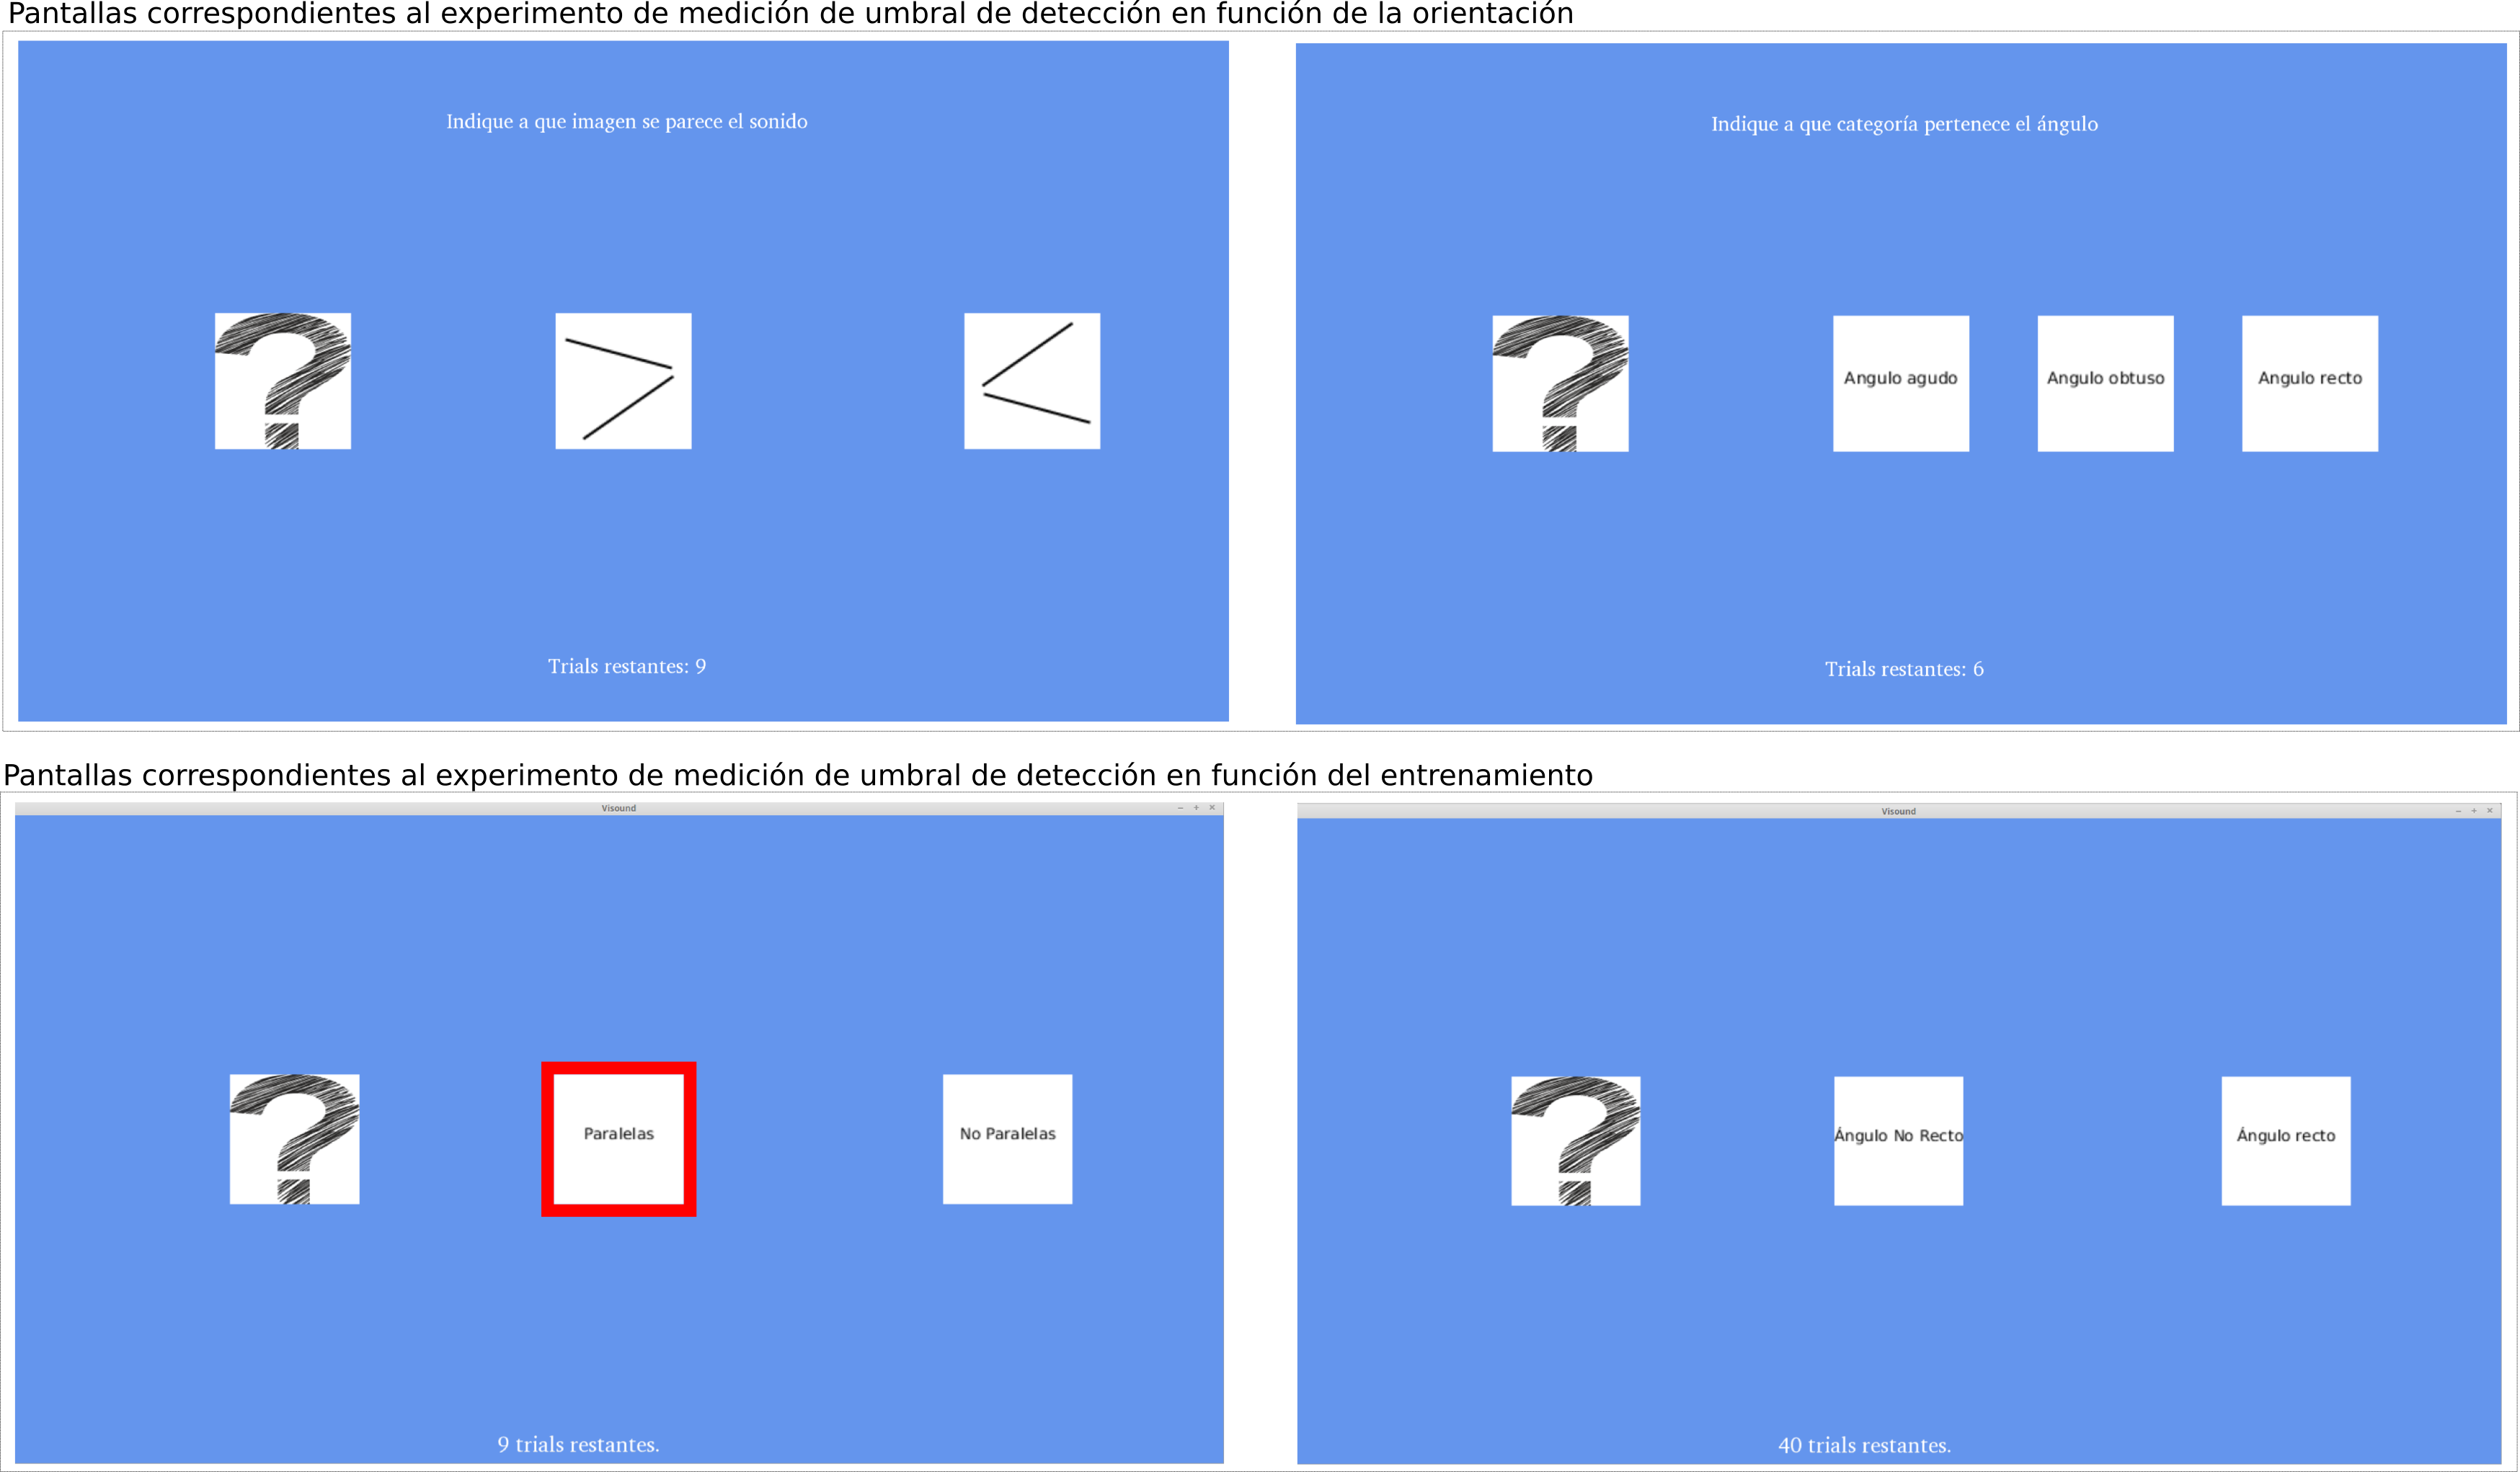
\includegraphics[width=\textwidth]{Imagenes/Pantallas2.png}
        \caption{Ejemplos de  capturas de pantalla de la aplicación correspondientes a las versiones con las que se realizaron los experimentos. Se observa que del primer al segundo experimento se modifico levemente el diseño de las preguntas para focalizar en la percepción o no de un aspecto especifico de la geometría en lugar de la distinción entre estímulos pertenecientes a categorías equivalentes. Este cambio se correspondió con un cambio en la lógica de construcción y selección de la muestra de estímulos durante los experimentos. En el segundo caso se muestra un ejemplo de feedback.}
        
        \label{fig:Pantallas2}
    \end{figure}
    
    \subsubsection{El registro de los datos}
    
    Los datos registrados por la aplicación fue variando según el avance del desarrollo de la misma. En un principio se decidió registrar todos los eventos necesarios para poder reconstruir por completo lo realizado por el usuario. Esta decisión resultó poco práctica porque involucraba la generación de un volumen de datos innecesario y ralentizaba todos los aspectos involucrados al envió y almacenamiento de los datos. 
    En versiones posteriores redujimos el registro realizado a la información más relevante. Si bien vario levemente debido a los cambios en el diseño experimental (que involucraron cambios en las estructuras de datos a enviar) el conjunto de datos registrados por la aplicación puede resumirse en lo siguiente:
    \begin{itemize}
        \item \textit{Registro de inicio de sesiones:} Este registro se realiza cada vez que el usuario inicia la aplicación. Se guarda el usuario (que si no existe se crea) identificado por un Id (la aplicación no identifica al usuario por su nombre o información personal), y un Id de la sesión, acompañado por información contextual de la aplicación (versión del código utilizado, etc) y del propio usuario (niveles ya realizados, etc)
        
        \item \textit{Registro de inicio de niveles:} Cada vez que el usuario inicia un nivel se genera y envía un registro con la información del nivel iniciado, un Id de dicho nivel (para diferenciar cada vez que se ejecuta el mismo nivel) y la información de contexto en que se inició dicho nivel (registro de la sesión)
        
        \item \textbf{Registro de Trials:} Al finalizar cada nivel, se guarda y envía toda la información referida a los Trials del nivel, en conjunto con toda la información general del nivel (Id del nivel, parámetros generales, etc). Según el diseño experimental utilizado en este envío se registran los resultados obtenidos para la medición esperada, y también una lista de todos los trials con sus estímulos y las respuestas seleccionadas. 
    \end{itemize}
    
    Para recolectar los datos se debía disponer de algún tipo de servidor disponible que fuera capaz de recibir los envíos de la aplicación y guardar la información. Si bien siempre se implementó una copia local de los registros, la idea era en un principio que la aplicación estuviera disponible en celulares donde era imposible acceder a los registro de los sujetos si no se envían. Para ello decidimos montar un servidor json-server \url{https://github.com/typicode/json-server} sencillo de instalar y que corre en casi cualquier computadora. El problema que tuvimos fue que la red de la institución donde trabajamos (Universidad Torcuato Di Tella) no permitía el acceso externo a un servidor montado en el laboratorio, por lo que decidimos dedicar un servidor externo (accesible a través de una IP hogareña a la que asociamos un dominio \url{http://turintur.dynu.com/} todavía activo) que corre en un sistema operativo raspbian en un dispositivo raspberry dedicado a tal efecto. Todos los registros generados (tanto en versión local como remota) siempre fueron almacenados en formato JSON (\url{http://www.json.org/}) que es un estándar muy difundido para guardar estructuras de datos en formato texto legible por humanos. 
    
    \subsubsection{Generación automática de la estructura de niveles, trials y estímulos} \label{seccion:builder}
    
    La generación de la estructura de niveles, Trials y estímulos fue desarrollándose a lo largo de las diferentes pruebas preliminares y experimentos, hasta converger a un proceso prácticamente automático que a partir de ciertos parámetros conceptuales es capaz de generar toda la estructura en forma consistente. Se describe a continuación y en forma conceptual los elementos y procedimientos que permiten tan tarea. 
    
    Es importante destacar que la lógica de creación de estímulos esta muy emparentada con el algoritmo StairCase descripto más adelante, este algoritmo se corresponde con los experimentos donde lo que se busca es medir es el umbral de detección de los sujetos, por lo tanto lo que hace falta es un conjunto de estímulos muy similares que aumenten gradualmente su característica distintiva (denominada señal en adelante). En el caso de las pruebas de paralelismo se va aumentando el ángulo formado por los segmentos y en el caso de las pruebas de ángulos se va haciendo al ángulo cada vez más diferente al ángulo recto (ver ejemplo en figura \ref{fig:Estimulos}). Este proceso re replica en muchas orientaciones diferentes.
    
    % Para la construcción de los recursos, cada clase (LevelEjemplos y LevelUmbralStatic) tiene su propio algoritmo. El LevelEjemplos es el nivel en el cual se muestran algunas imágenes arbitrarias para que el usuario pueda escuchar como suenan, por esta razón, los recursos y trials se generan por extensión habiendo elegido algunos recursos que nos parecieron ilustrativos de la lógica del vOCIe. En cambio la clase LevelUmbralStatic (que incluye los dos niveles sencillo que para el usuario se denominan tutorial) se crea por completo en forma parametrica. 
    
    %La clase LevelEjemplos posee en su código un listado de los Trials necesarios donde se especifica en cada trial los estimulos que lo conforman. Por otro lado posee un listado de los estimulos a generar que se armaron en forma manual. Con esta información al ejecutarse el metodo buildLevel convoca a la clase Imagen una vez por cada recurso necesario pasandole en los parametros las coordenadas de las lineas a crear, esta clase crea un archivo en disco en formato SVG por cada imagen. Por otro lado con la información de los trials, crea la estructura de datos necesaria y vuelca en disco la información del nivel y los trials. Concluido el proceso de creacion de archivos SVG y de trials se ejecuta el SVGtoMP3 para transformar la información al formato adecuado. 
    
    %La clase LevelUmbralStatic incluye un proceso mas complejo. Lo primero que realiza es un reconocimiento de todos los tipos de niveles que se desean crear (tutorial, test, entrenamiento) ya que cada tipo de nivel tiene parámetros diferentes en los trials. Por otro lado busca que tipo de estímulos usa cada tipo de nivel para crear los estímulos necesarios (diferentes niveles pueden usar los mismos estímulos). Un ejemplo de los estímulos creados para el tutorial (son pocos estímulos porque sirven solo de ejemplo a la lógica de la aplicación) se puede ver en la figura \ref{fig:Estimulos}
    
        
    \begin{figure}
        \center
        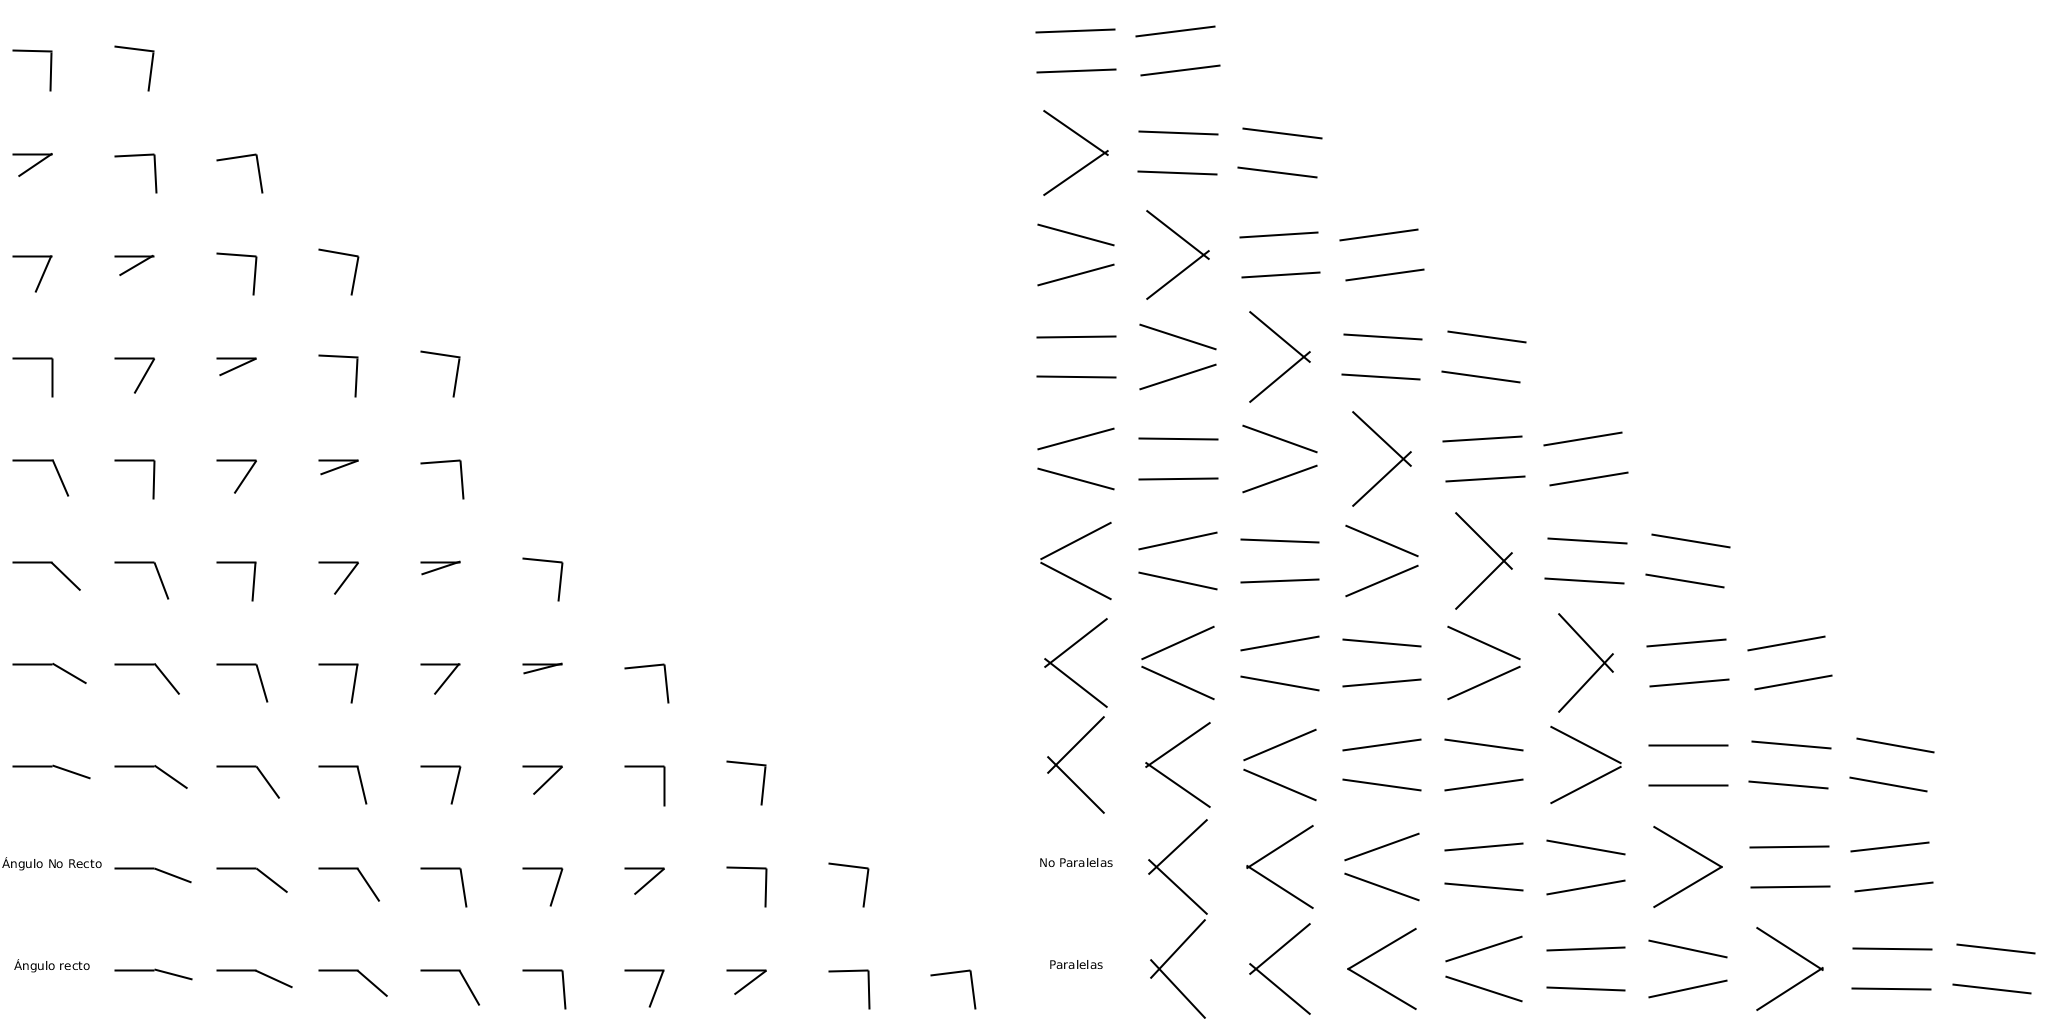
\includegraphics[width=\textwidth]{Imagenes/Estimulos.png}
        \caption{Ejemplo de imágenes creadas en forma paramétrica como estímulos en los últimos experimentos de ángulos y de paralelismo. Estas imágenes corresponden al nivel de tutorial por lo que la serie es reducida. En los niveles de evaluación se generan muchas mas variantes. En este caso, el ángulo de referencia es de 0º para paralelismo y de 180º para ángulos. La variación del estimulo (o nivel de señal) entre figura y figura es lineal y va de 0 a 80º para los ángulos (no rectos) y de 0º a 100º para las paralelas (no paralelas). Además se crearon 18 estímulos 'sin señal' (rectos y paralelas) levemente rotados para intercalar entre los estímulos con señal.}
        \label{fig:Estimulos}
    \end{figure}
    
    
    Para la creación de los estímulos se consideran los siguientes parámetros: 
    \begin{itemize}
        \item \textit{numero de estímulos por serie:} Especifica cuantos estímulos diferentes se deben crear en cada orientación (en el caso de la figura \ref{fig:Estimulos} vale 20). Cada elemento de esta serie difiere solamente en la intensidad de la señal del estimulo. En el caso de las paralelas la señales es el ángulo entre ambas. En el caso de los ángulos es el cuanto mayor o menor que el ángulo recto es.
        \item \textit{ángulos de referencia:} En el caso de paralelas es la dirección en que apunta la mediatriz, en el caso de los ángulos, la dirección en que apunta el lado que no se modifica. En el ejemplo de la figura \ref{fig:Estimulos} valen 0º y 180º. En los niveles correspondientes al último experimento realizado estos ángulos valen 30º, 60º, 120º y 150º (ver figura \ref{fig:simetrias}) 
        \item \textit{Deviaciones angulares:} Lista de pequeñas rotaciones que se utiliza para generar mayor variabilidad en los estímulos. En la figura \ref{fig:Estimulos} no se genero ninguna variabilidad por ser un tutorial, pero en general se generaron muchas series similares con fluctuaciones de $\pm$ 2.5º y $\pm$ 5º en la referencia para evitar que el sujeto se acostumbrara a reconocer sonidos de memoria (ver más detalles en el diseño experimental de la última medición, sección \ref{seccion:Exp2_Diseno})
        \item \textit{Fluctuaciones estimulo neutro:} Lista de pequeñas rotaciones usadas para generar variabilidad en el estimulo que no posee señal (estímulo neutro) de manera de evitar acostumbramiento. En general usamos un rango de $\pm$ 10º  (ver más detalles en el diseño experimental de la última medición, sección \ref{seccion:Exp2_Diseno}))
        \item \textit{Señal máxima:} Máximo valor de señal a alcanzar en cada serie (con signo positivo y negativo)
        \item \textit{Señal mínima:} Mínimo valor de señal a alcanzar en cada serie (con signo positivo y negativo)
        \item \textit{Escala logarítmica:} Establece si se utiliza una escala logarítmica en el cambio de la señal o una lineal. En un principio usamos logarítmica, pero luego lineal. 
    \end{itemize}
    
    Con esta lista de parámetros que se pueden configurar para cada diseño experimental, la clase LevelUmbralStatic lo que hace es generar todas las combinaciones posibles de estímulos. Para cada uno de esos estímulos crea los segmentos que lo componen y ejecuta el código que arma el correspondiente archivo SVG. Además para cada estímulo creado hace un análisis de los parámetros y crea un archivo de información conceptual donde almacena las categorías a las que pertenece ese estímulo junto con detalles de su conformación y los parámetros utilizados. También en forma simultanea ordena los estímulos por señal (y orientación) y crea un registro centralizado que es guardado en disco y será posteriormente utilizado por el creador de Trials y por el algoritmo que manipula los niveles en tiempo de ejecución.
    
    Una vez creados todos los estímulos el constructor de niveles revisa que niveles se desean crear, y que estímulos utilizan. Con esta información crea un trial para cada estimulo utilizado, en forma automática, donde configura el trial (con o sin feedback, si se reproduce el estimulo en loop, etc) según que tipo de nivel se trate (los niveles están agrupados en categorías según su comportamiento: tests, tutorial, entrenamientos). También durante la creación de los trials registra que estimulo esta asociado a cada trial de forma que posteriormente el programa sepa que trial cargar cuando decida mostrar cada estimulo. 
    
    \subsection{Medición del umbral de detección: adaptación de un algoritmo tipo StairCase.}
    \label{seccion:staircase}
    
    Como se menciono en el panorama general del trabajo realizado, una vez hechas las primeras mediciones y habiendo comprobado que los usuarios eran capaces de distinguir entre figuras con grandes diferencias (ver figura \ref{fig:ResultadosPreliminar}) necesitábamos encontrar alguna manera de cuantificar la dificultad de reconocer los estímulos sabiendo que muy probablemente dicha dificultad dependiera de cada sujeto. Lo que queríamos era establecer una escala de dificultad y observar en que valores de dicha escala cada usuario dejaba de poder distinguir entre dos estímulos cuantitativamente similares pero cualitativamente diferentes. Para resolver este tipo de problemas existen algoritmos y mecanismo ya desarrollados, por ejemplo los tipo Quest, pero esta solución no nos servía ya que la implementación debía ser compatible con nuestro entorno de programación en LibGDX, ya que la base de estos algoritmos está en seleccionar en forma dinámica (según las respuestas del sujeto) que estímulos se muestran y eso necesariamente debía estar incluido en el código que se ejecuta en tiempo real. 
    
    Por esta razón decidimos apelar a algunos algoritmos similares pero más sencillos cuya implementación pudiera ser reproducible programando desde cero la lógica de funcionamiento en nuestro propio entorno. Para eso decidimos implementar algún algoritmo tipo StairCase, cuya base funcional se puede consultar en el paper "Transformed Up-Down Methods in Psychoacoustics"\cite{staircase} de H Levitt de 1970. Sobre esta idea fuimos realizando sucesivas pruebas para adaptar esta lógica a nuestras necesidades. 
    
    La idea básica del StairCase es cuantificar los estímulos en función del aspecto que se quiere identificar y ordenarlos de mayor a menor. A esa escala la llamaremos señal. Luego, tomar alguna muestra inicial y pedirle al sujeto que reporte si detecta la característica o no. Si el sujeto detecta la característica se selecciona un estimulo que posea dicha característica en grado menor y se repite la prueba, si el sujeto reporta que no detecto la característica se toma una muestra que la posea en mayor grado y así sucesivamente. Con ciertos cuidados y asumiendo cierto rango de error, la secuencia de pruebas (o trials) debería converger al nivel de señal en el cual el sujeto pasa de percibir a no percibir lo deseado. 
    
    En el primer experimento donde probamos implementar este algoritmo, queríamos medir el umbral de 
    detección de paralelismo (es decir la capacidad de distinguir si dos segmentos son paralelos o no). Para eso podíamos mostrar segmentos cada vez mas paralelos pero el problema era que si el sujeto sabe (o se da cuenta) que los segmentos son cada vez mas paralelos va a responder siempre que no son paralelos. Y si intercalamos estímulos paralelos entre los no paralelos va a haber siempre un estimulo repetido, fácilmente reconocible por un efecto memoria. 
    
    La solución encontrada fue generar estímulos no paralelos hacia un lado o hacia el otro, e intercalar (al azar) entre ambos tipos estímulos. De esta manera, preguntando no si eran paralelos o no, sino hacia que lado se juntaban (ver figura \ref{fig:Pantallas2} a modo de ejemplo) podíamos intercalar estímulos de manera que el sujeto no pudiera tener un criterio de elección que no fuera la percepción a estudiar para responder entre las opciones. Un aspecto a tener en cuenta, es que tal como fue enunciado el algoritmo falla, pues debe considerar la probabilidad de que el sujeto responda bien, incluso cuando no pueda distinguir entre las opciones por solo efecto del azar. La solución a este último punto es reducir la señal del estimulo, no cuando el sujeto responde bien, sino cuando responde bien en mayor proporción que mal. De esta manera respuestas aleatorias hacen que el desempeño del sujeto sea cada vez menor. 
    
    Otro aspecto importante a considerar en el desarrollo y la optimización del algoritmo, es la rapidez con que converge. Porque si bien en teoría a la larga el algoritmo puede estabilizarse, a la hora de tomar mediciones con sujetos que se cansan, o que aprenden sobre la marcha, es importante que la convergencia sea rápida. Sobre todo si se quieren tomar muchas mediciones sucesivas (en diferentes orientaciones) como era nuestro caso. Para eso una solución abordada fue realizar saltos más grandes de dificultad en un principio cuyo valor fuera disminuyendo con el tiempo hasta reducirse al mínimo (máxima resolución) cuando se asume que la señal debería estar convergiendo al nivel de umbral. 
    
    \subsubsection{Primer versión del algoritmo} \label{staircase1}
    
    Como compromiso entre todos estos factores encontramos una primera versión del algoritmo que para una secuencia de 40 pruebas mostró resultados aceptables. En forma cualitativa el algoritmo realizaba lo siguiente:
    
    \begin{enumerate}
        \item Punto de partida:
        \begin{itemize}
            \item Se dispone de una serie de estímulos ordenados por nivel de señal que se encuentran repartidos entre un valor máximo y uno mínimo. 
            \item Hay mas de un estimulo por nivel de señal (al menos dos, en nuestro caso segmentos cuasi paralelos apuntando hacia lados diferentes) que se pueden distinguir con mayor o menor facilidad en función de la señal. 
            \item Se configura el nivel de señal en el extremo mas fácil de la escala. 
            \item Se configura el salto inicial en un décimo de la cantidad de estímulos de dificultad diferente.
        \end{itemize}
        \item Se muestra un estimulo. \label{algo:dos}
        \item Se registra y almacena si la respuesta fue correcta.
        \item Si hay al menos dos respuestas se compara las últimas dos, si son diferentes (es decir una bien y una mal, un rebote) se disminuye el nivel del salto salvo que este ya sea igual a 1.
        \item Si la respuesta fue incorrecta se aumenta la señal (estimulo mas fácil) en lo que indique el salto. Si fue correcta y el salto es mayor a 1 se disminuye la señal (estimulo más difícil). Si el salto es igual a uno, solo se disminuye la señal si hay al menos dos respuestas correctas consecutivas.  
        \item Si la señal se va de rango se la coloca en el estimulo mas fácil o mas difícil según corresponda. 
        \item Una vez regulado el nivel de señal se busca al azar entre los estímulos uno nuevo que tenga el nivel de señal correspondiente. 
        \item Se vuelve al paso \ref{algo:dos} o si se llega a los 40 trials se detiene el algoritmo (y el nivel)
    \end{enumerate}
    
    Resumiendo, se realiza un ajuste del nivel de señal con saltos grandes que van decreciendo cuando se detectan rebotes. Una vez que el salto es la mínima distinción entre estímulos dos aciertos consecutivos aumentan la dificultad y un error la disminuye. El algoritmo debería estabilizarse donde al sujeto le cuesta distinguir entre los estímulos y tiene chance aproximada de 0.7 de reconocerlo bien. 
    
    \begin{figure}
        \center
        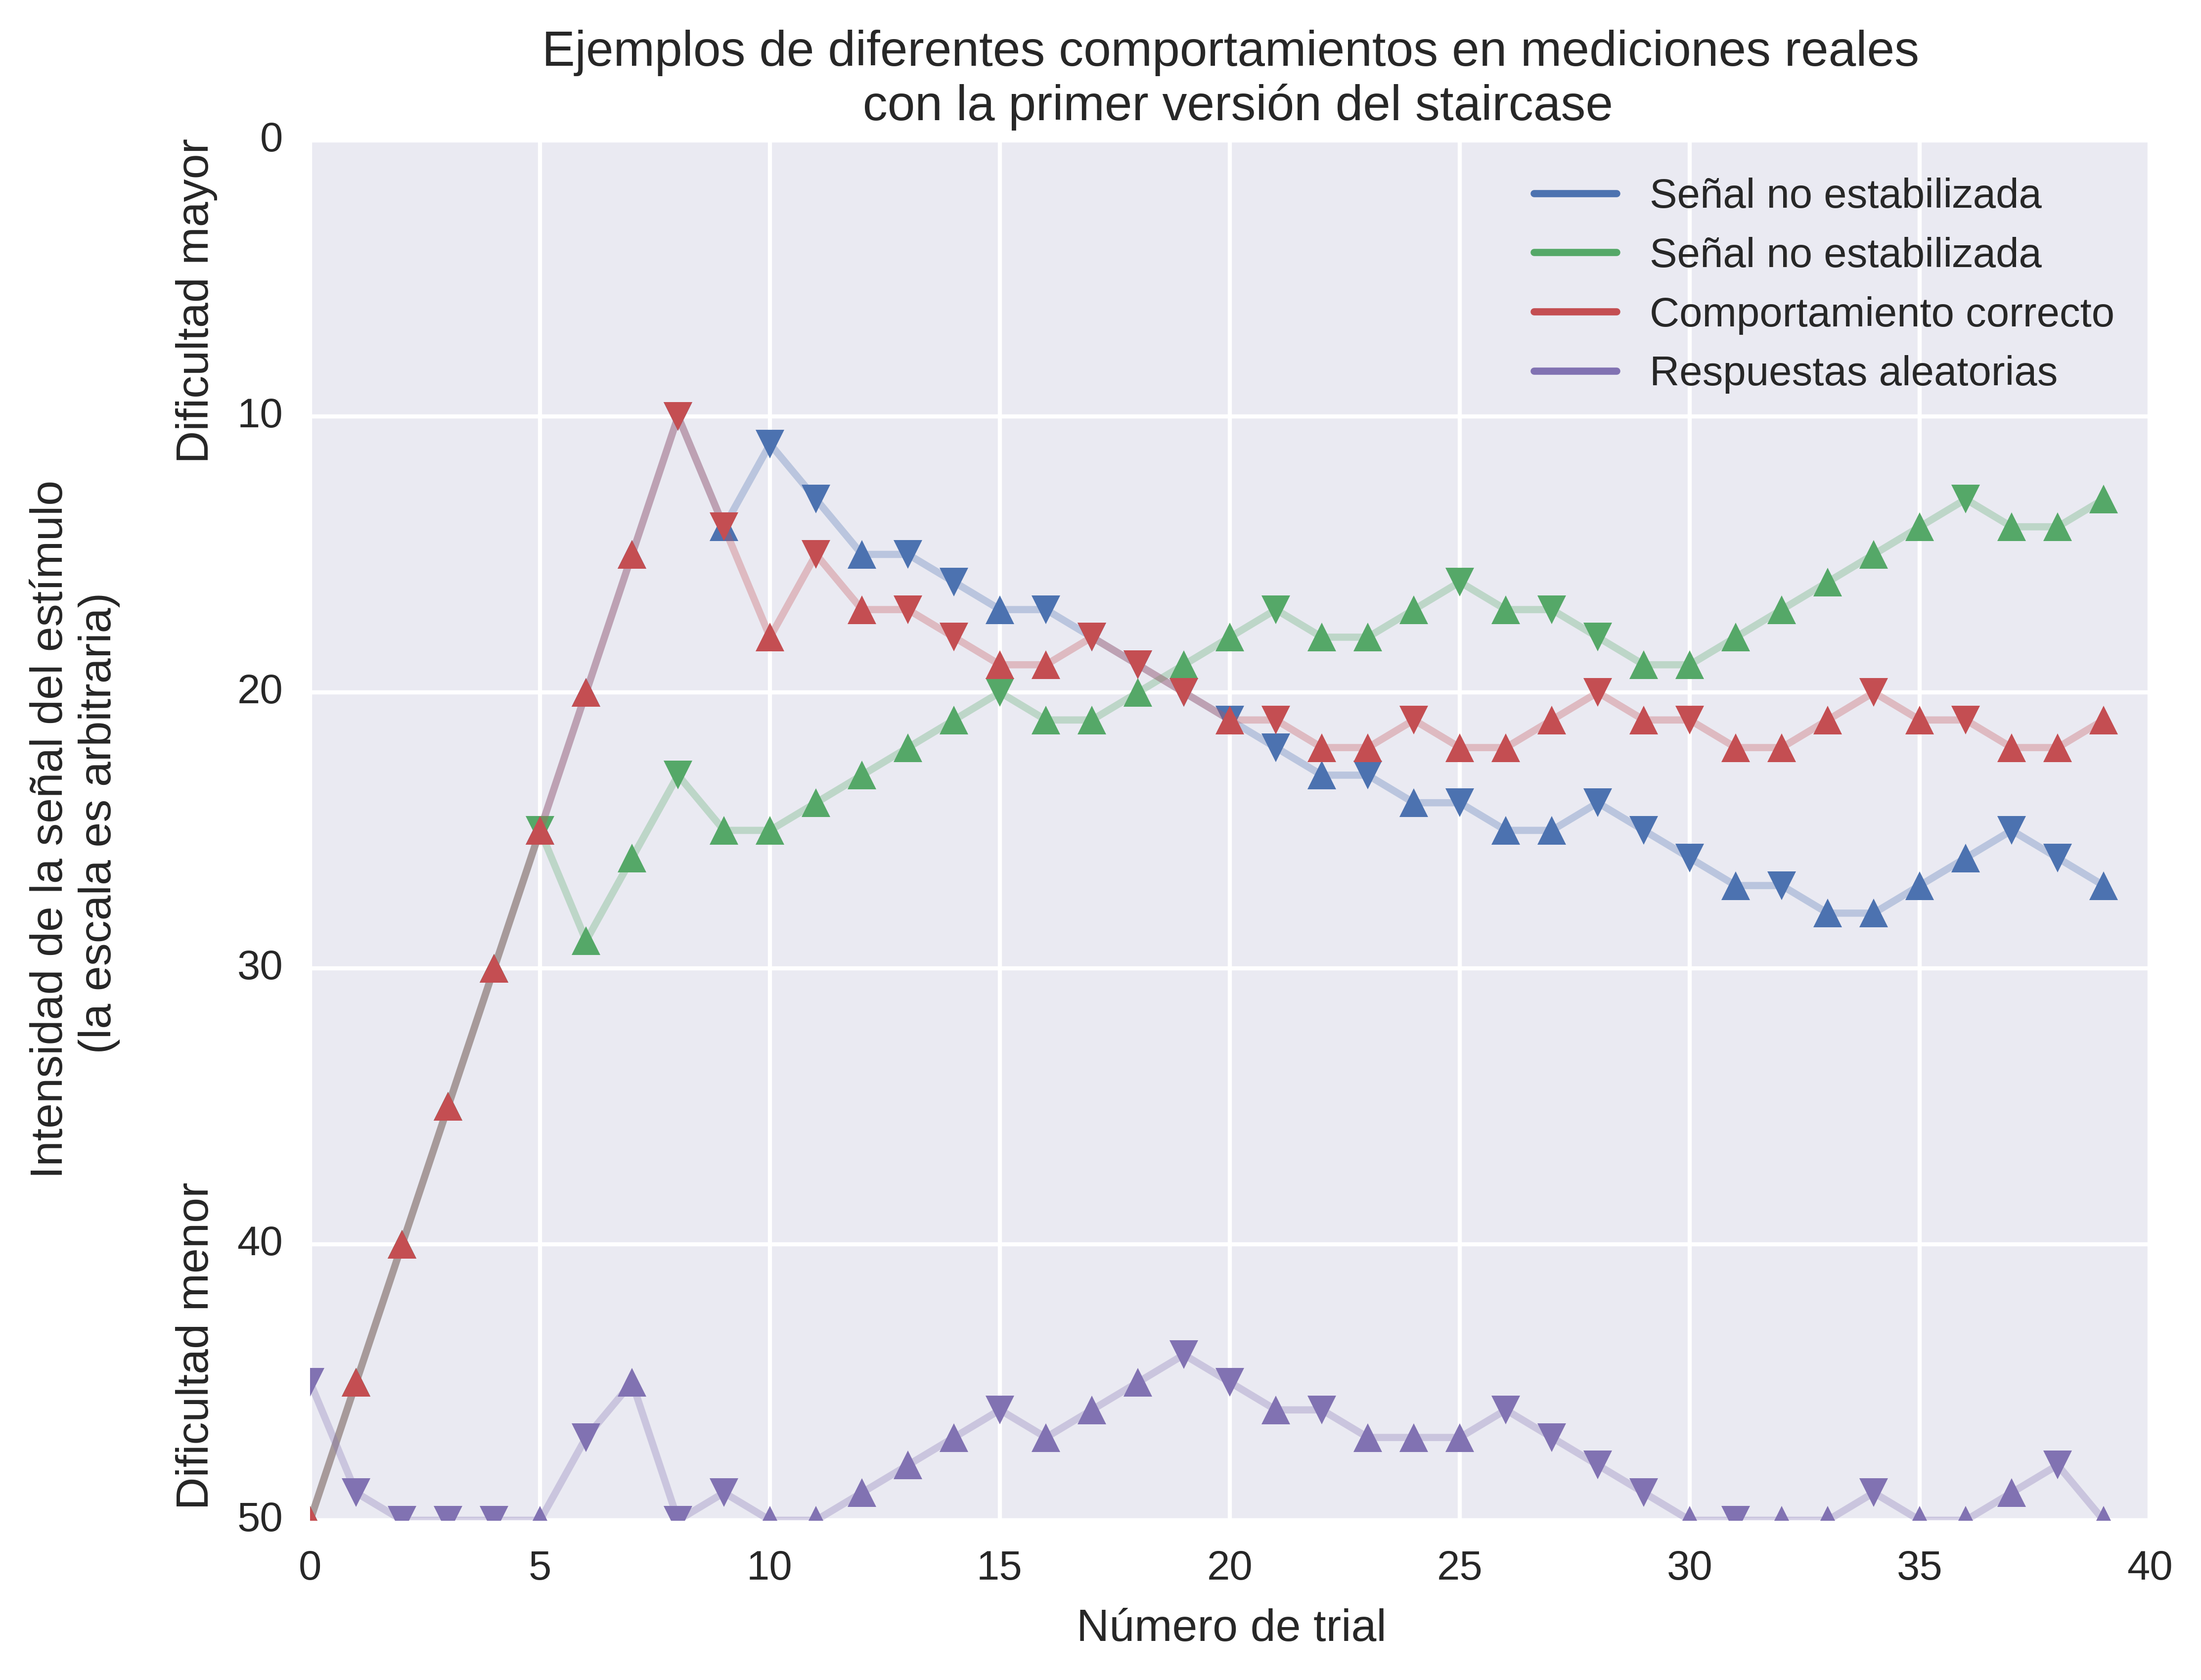
\includegraphics[width=\textwidth]{Imagenes/StairCase1.png}
        \caption{Ejemplos reales de mediciones preliminares, donde se observa como se regula la señal mostrada en cada trial en función de las respuestas previas. En la figura los triángulos hacia arriba indican una identificación correcta del estimulo, los que apuntan hacia abajo una incorrecta. La lógica del algoritmo se corresponde con la primera versión de StairCase que se detalla en la sección \ref{staircase1}. Cada serie corresponde a una orientación diferente donde el rango de las señales reales (medidas según el parámetro de la figura geométrica) no es el mismo, ni guarda relación lineal con la escala del algoritmo, solo respeta el orden de dificultad.}
        \label{fig:staircase1}
    \end{figure}    

    \subsubsection{Segunda versión del algoritmo} \label{staircase2}
    
    \begin{figure}
        \center
        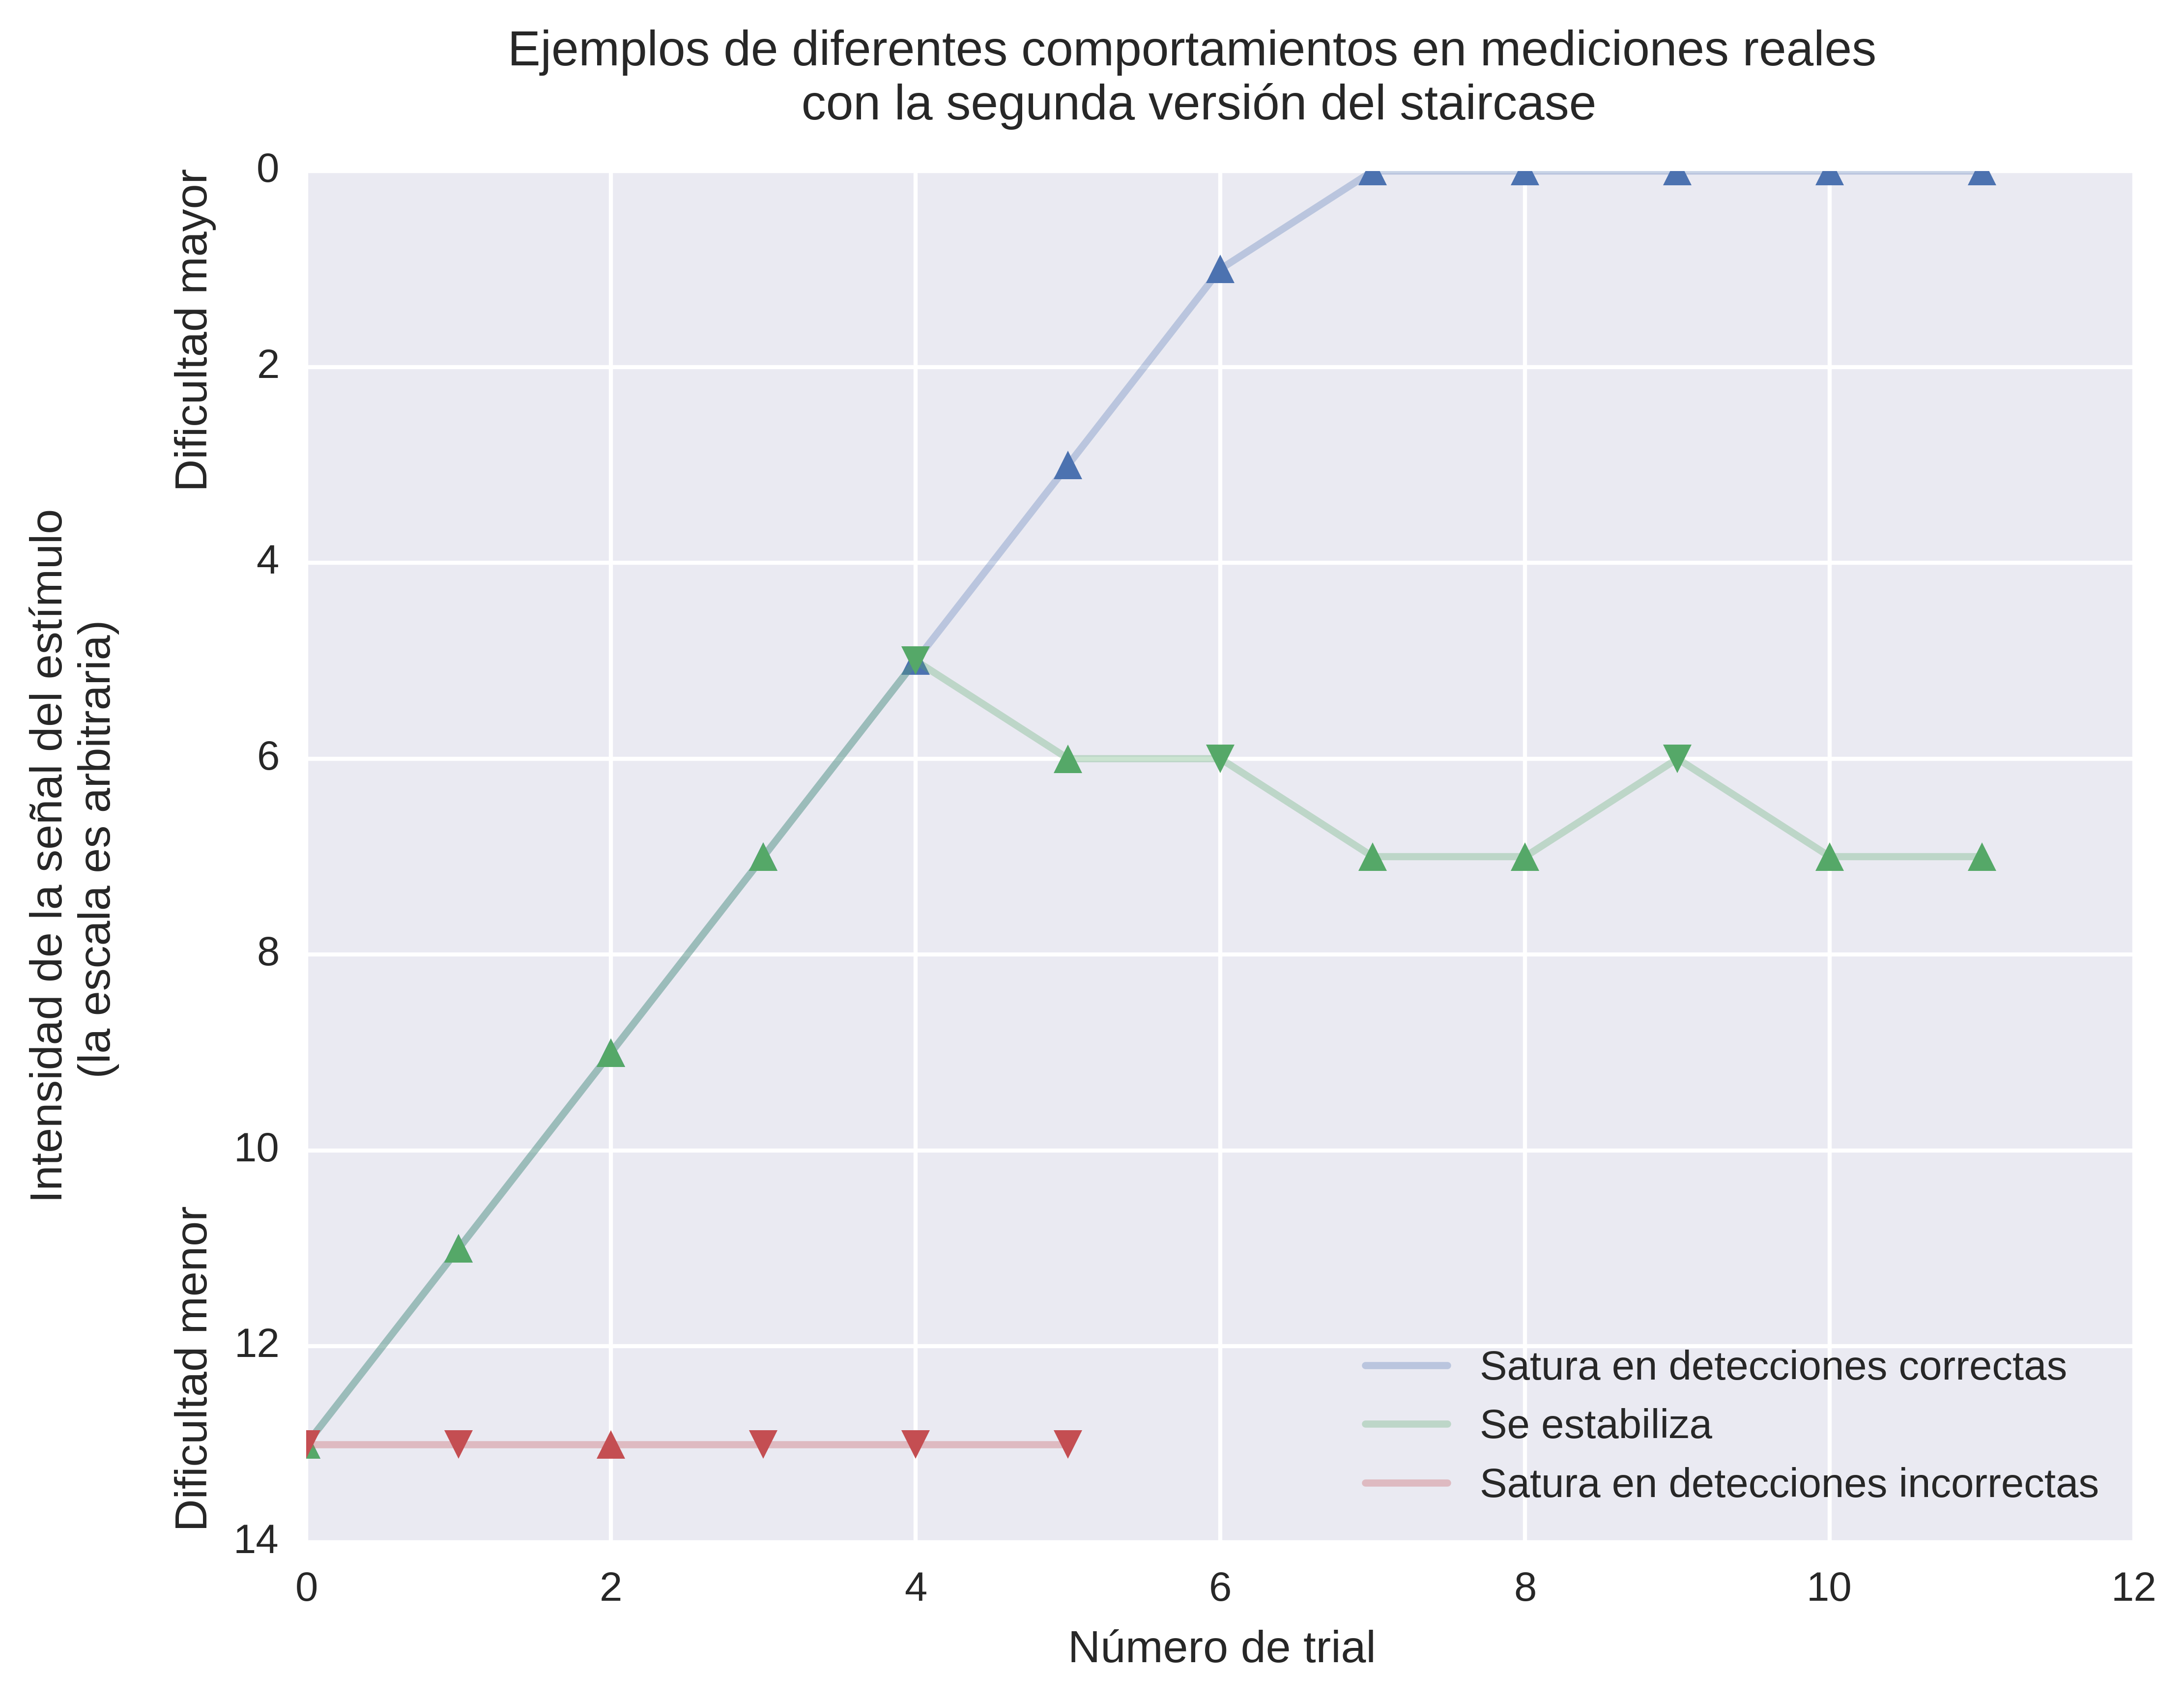
\includegraphics[width=\textwidth]{Imagenes/StairCase2.png}
        \caption{Ejemplos reales de mediciones en el experimento de dependencia con la orientación con el algoritmo detallado en la sección \ref{staircase2}. Todas las mediciones mostradas son en detección de ángulos. Se observa que hubo una baja densidad de estimulos diferentes y que en algunos casos los sujetos reconocieron sistemáticamente mal los estímulos}
        \label{fig:staircase2}
    \end{figure}  
    
    Pese a que el algoritmo mencionado en la sección anterior resultó funcional y permitió realizar las primeras pruebas, nos encontramos con que los experimentos eran demasiado largos (duraban alrededor de cuatro horas). Si bien la razón de esta duración era principalmente debido a motivos externos al algoritmo de búsqueda del umbral, intentamos realizar modificación tendientes a acortar la cantidad de pruebas necesarias para poder determinar el nivel de umbral. 
    
    Como la lógica a la que queríamos apuntar era mas compleja, y además por motivos experimentales (evitar el acostumbramiento) queríamos poder intercalar pruebas con estímulos pertenecientes a diferentes orientaciones similares, creamos (a imitación de ciertos algoritmos tipo Quest en Matlab) una clase especifica (denominada 'DinamicaExperimento') para manipular la información de la secuencias de trials realizados. Esto permitía manejar en forma diferenciada la convergencia de cada serie de mediciones conservando en cada una la información relevante. Básicamente se desdobló el funcionamiento del loop principal del programa que convoca un trial tras otro del de la lógica interna del StairCase correspondiente a cada conjunto de estímulos. De esta manera en cada nivel se podían crear tantos algoritmos de convergencia como fuera necesario, y si bien en el diseño del experimento finalmente realizado no se intercalo estímulos de orientaciones diferentes, si se desdoblo los estímulos que se aproximan al neutro desde cada 'lado' (en el caso de ángulos aproximándose al recto desde agudos u obtusos y en el caso de paralelismo según hacia que lado se juntaran).
    
    Además para evitar mediciones innecesarias en series de trials que se asumiera que ya habían convergido a un valor estable, se diseño un criterio de corte. Este diseño (que después resultó ser poco práctico) consistía en hacer un análisis de los últimos trials realizados y observar si la desviación estándar de los valores de la señal (siempre en una escala lineal de paso 1) estaba por debajo de cierto umbral. El rango de trials a considerar y el valor de desviación considerado como limite se estableció experimentalmente realizando múltiples pruebas para cada uno de estos valores. Otra modificación que se estableció fue en la rapidez con que se reducía el salto de señal entre trial y trial, haciendo que se disminuyera solo en uno de cada dos rebotes (es decir solo cuando observaba la secuencia: Acierto-Error), de esta manera se buscaba evitar que algunos desacierto al comienzo de la serie (debido a la falta de comprensión de la tarea) hicieran que el nivel quedara muy lejos del objetivo y no llegara a converger en el numero de trials limite. A su vez incluimos una variable para determinar cuantos aciertos consecutivos debían darse antes de cambiar a un estimulo mas difícil. 
    
    En base a pruebas y calibraciones, se utilizó un numero variable de estimulos de intensidad diferentes según la orientación para las pruebas de ángulos y de 40 para las de paralelismo (ver mas detalles de la configuración experimental en la sección \ref{seccion:Exp1}). Al igual que antes se comenzaba con el estímulo mas sencillo de reconocer, y el salto inicial fue configurado en un décimo de los estimulos totales diferentes. Se considero un secuencia de dos detecciones correctas para aumentar la dificultad y una para disminuirla, y para establecer el criterio de corte se considero la señal de los últimos seis estimulos y una desviación estandar menor a 0.5 en dichos valores (donde la unidad es un paso en el cambio de intensidad de señal independientemente de que represente esto en el aspecto geométrico de los estimulos).

    \subsubsection{Versión final del algorítmo} \label{staircase3}
    
    Tras observar los resultados (en tanto desempeño del algoritmo y diseño general) del experimento que se hizo con el algoritmo descrito en \ref{staircase2}, decidimos implementar varios cambios, lo cual como sucedió a lo largo de todo el trabajo también estuvo acompañado por motivaciones en el diseño experimental de la siguiente medición.
    
    Por un lado la idea de cortar la duración del staircase en función del desempeño no resulto buena, ya que genero mucha fluctuación de cualquier análisis estadístico que comparara mediciónes. Por otro lado ya sabíamos que los experimentos como los estábamos diseñando no resultaban tan largos como temíamos en un principio, por lo que no era necesario implementar un recorte en el numero de estímulos mostrados. Si en cambio detectamos como falencia en el metodo anterior el bajo numero de estímulos diferentes y por ende la poca resolución inherente al método de medición. Esto no fue un problema serio para el experimento anterior pero al diseñar un experimento que permitiera medir la mejora en el desempeño de cada sujeto era un limitante a corregir. Otro aspecto que se descubrió inadecuado fue el haber elegido una escala logarítmica en la representación de la dificultad de los estímulos ya que en la zona lejana a los ejes cartesianos (donde pensábamos realizar el entrenamiento) los individuos presentaron mucha fluctuación en su capacidad de detección y por lo tanto no tenia sentido establecer una escala que a priori estableciera una resolución mayor en una zona sin saber en que valores estaría el umbral de cada sujeto. Todas estas razones nos indujeron a implementar un algoritmo con mucha mayor cantidad de estímulos y con un proceso de convergencia más rápido. 
    
    Otro cambio importante para el funcionamiento del algoritmo fue que por el cambio en el diseño experimental, podíamos generar variedad de estimulos de señal equivalente, así como variedad de estímulos de señal cero (o neutros). Esto hizo que el tipo de pregunta conceptual a responder en cada trial fuera conceptual (detección o no de las categorías paralelo/no paralelo y recto/no recto), de esta manera era necesario un solo staircase por nivel. A su vez, en este diseño experimental decidimos incluir estimulos fáciles (CatchTrials) para eventualmente poder distinguir a los sujetos que tenían un mal desempeño de aquellos que no entendían la tarea. Cabe aclarar que el diseño de esta versión del staircase debía prever que en el experimento propuesto habría diferentes etapas experimentales, algunas de evaluación y otras de entrenamiento, de diferente duración cada una.
    
    En base a lo expuesto se ideó un algoritmo que se puede consultar en el anexo (sección:  \ref{anexo:staircase}) cuyos puntos más relevantes son los siguientes:
    
    \begin{itemize}
        \item ESe busco tener siempre la misma cantidad de estimulos equivalentes. Para esto se genera una lista pseudoaletoria bien balanceada (entre CatchTrials, estimulos con señal y estimulos neutros o sin señal) que establezca que tipo de estímulo mostrar en cada trial independiente del nivel de señal en que se encontrara el staircase. 
        \item Los estímulos son catalogados por su nivel de señal durante la generación de estimulos y niveles. Para cada intensidad de señal se dispone de varios estímulos. Por lo tanto conocido el nivel de señal a mostrar se debe seleccionar al azar un estimulo con la señal correspondiente o bien uno neutro (también elegido al azar). Aunque el estimulo neutro sea siempre seleccionado sobre un mismo conjunto reducido de estimulos, esto no representa un problema, ya que el objetivo del staircase es determinar cuando el sujeto deja de percibir el contraste entre estimulos con y sin señal. Por lo tanto, para las zonas donde el estimulo es bajo (en relación a la capacidad del sujeto) es tan difícil distinguir si un estimulo con señal baja no es neutro como si un estimulo neutro no tiene señal baja.
        \item El funcionamiento del staircase se pensó en tres etapas consecutivas, la primera con un salto muy grande que sirviera para sacar al staircase del valor inicial aproximándolo a un valor representativo del desempeño del usuario, de manera rápida, independientemente de la densidad de estimulos existentes (que modifican el rango y numero de valores que toma la variable que llamamos señal). Para eso los saltos en la primer etapa son proporcionales al numero total de pasos que puede tomar la señal. 
        \item Durante la primer etapa el salto decae linealmente hasta alcanzar el valor que debe tener en la segunda etapa. Además todos los estimulos (excepto los CatchTrial) generan un salto en la señal según sean aciertos o no. Esta primer etapa puede concluir anticipadamente si hay muchos rebotes o bien si ya se conoce un valor esperado de umbral en cuyo caso la etapa se saltea y directamente se inicia la secuencia en el valor esperado. Esto sucede durante los entrenamientos cuando el mismo sujeto realiza muchas veces niveles similares. 
        \item La segunda y tercer etapa tienen saltos que son independientes del rango total porque asumen que ya se esta cerca del valor esperado y se enfocan en conseguir un nivel estable de señal. La diferencia entre ambas es un factor de escala en los saltos. Mientras que la última hace saltos lo mas pequeños posibles para maximizar la resolución, la anterior los hace un poco mas grandes para acelerar la convergencia. 
        \item Durante las dos ultimas etapas básicamente reprodujimos el código para matlab que implementa la logica descrita en el paper de Levitt\cite{staircase} disponible en \url{https://github.com/lugtigheid/matlabstaircase}. 
        \item El cambio que introduce este código respecto a nuestra implementación previa de un StairCase es que respeta cuidadosamente la proporción entre aciertos y errores esperados en el umbral. Básicamente la diferencia es que reinicia el contador de aciertos o errores tras cada salto, con lo cual por ejemplo una secuencia de cuatro aciertos consecutivos que anteriormente producía tres saltos, ahora produciría dos (asumiendo dos aciertos o un error para para generar un salto). A su vez, la modificación que realizamos fue que incrementamos el nivel del salto en forma proporcional a la cantidad de saltos dados (en la misma dirección). Esta corrección permite acelerar la convergencia si la señal quedo fuera del rango adecuado y por lo tanto hay muchos aciertos o errores consecutivos, modificando la resolución del algoritmo pero no su estadística.
        \item Los CatchTrials que se intercalan en la secuencia (cuando el orden pseudorandom lo indica) no son considerados por el análisis del StairCase, aunque si se regula su dificultad en relación al nivel de señal que detecta el sujeto. Elegimos como criterio que el CatchTrial se encuentre en algún valor aleatorio de dificultad entre la mitad mas fácil de los estimulos y que sea al menos el doble de 'fácil' que el nivel en que se encuentra la señal del staircase.
        
    \end{itemize}
    
    En la figura \ref{fig:staircase3} se observan algunos ejemplos de los resultados obtenidos con este algoritmo. Como se puede ver, no siempre las mediciones dieron los resultados esperados (aunque en la mayoría de los casos si se estabiliza la medición), sin embargo es difícil definir si esto se debe a una falla estadística en su ejecución o a que los sujetos a veces tardan en reconocer la tarea a realizar, o bien reflejan efectos de cansancio. Debido al método implementado por el algoritmo su mayor falencia está en ser poco sensible a correcciones que deban reflejar mejoras en el rendimiento del sujeto una vez avanzado el nivel. 
    
    \begin{figure}
        \center
        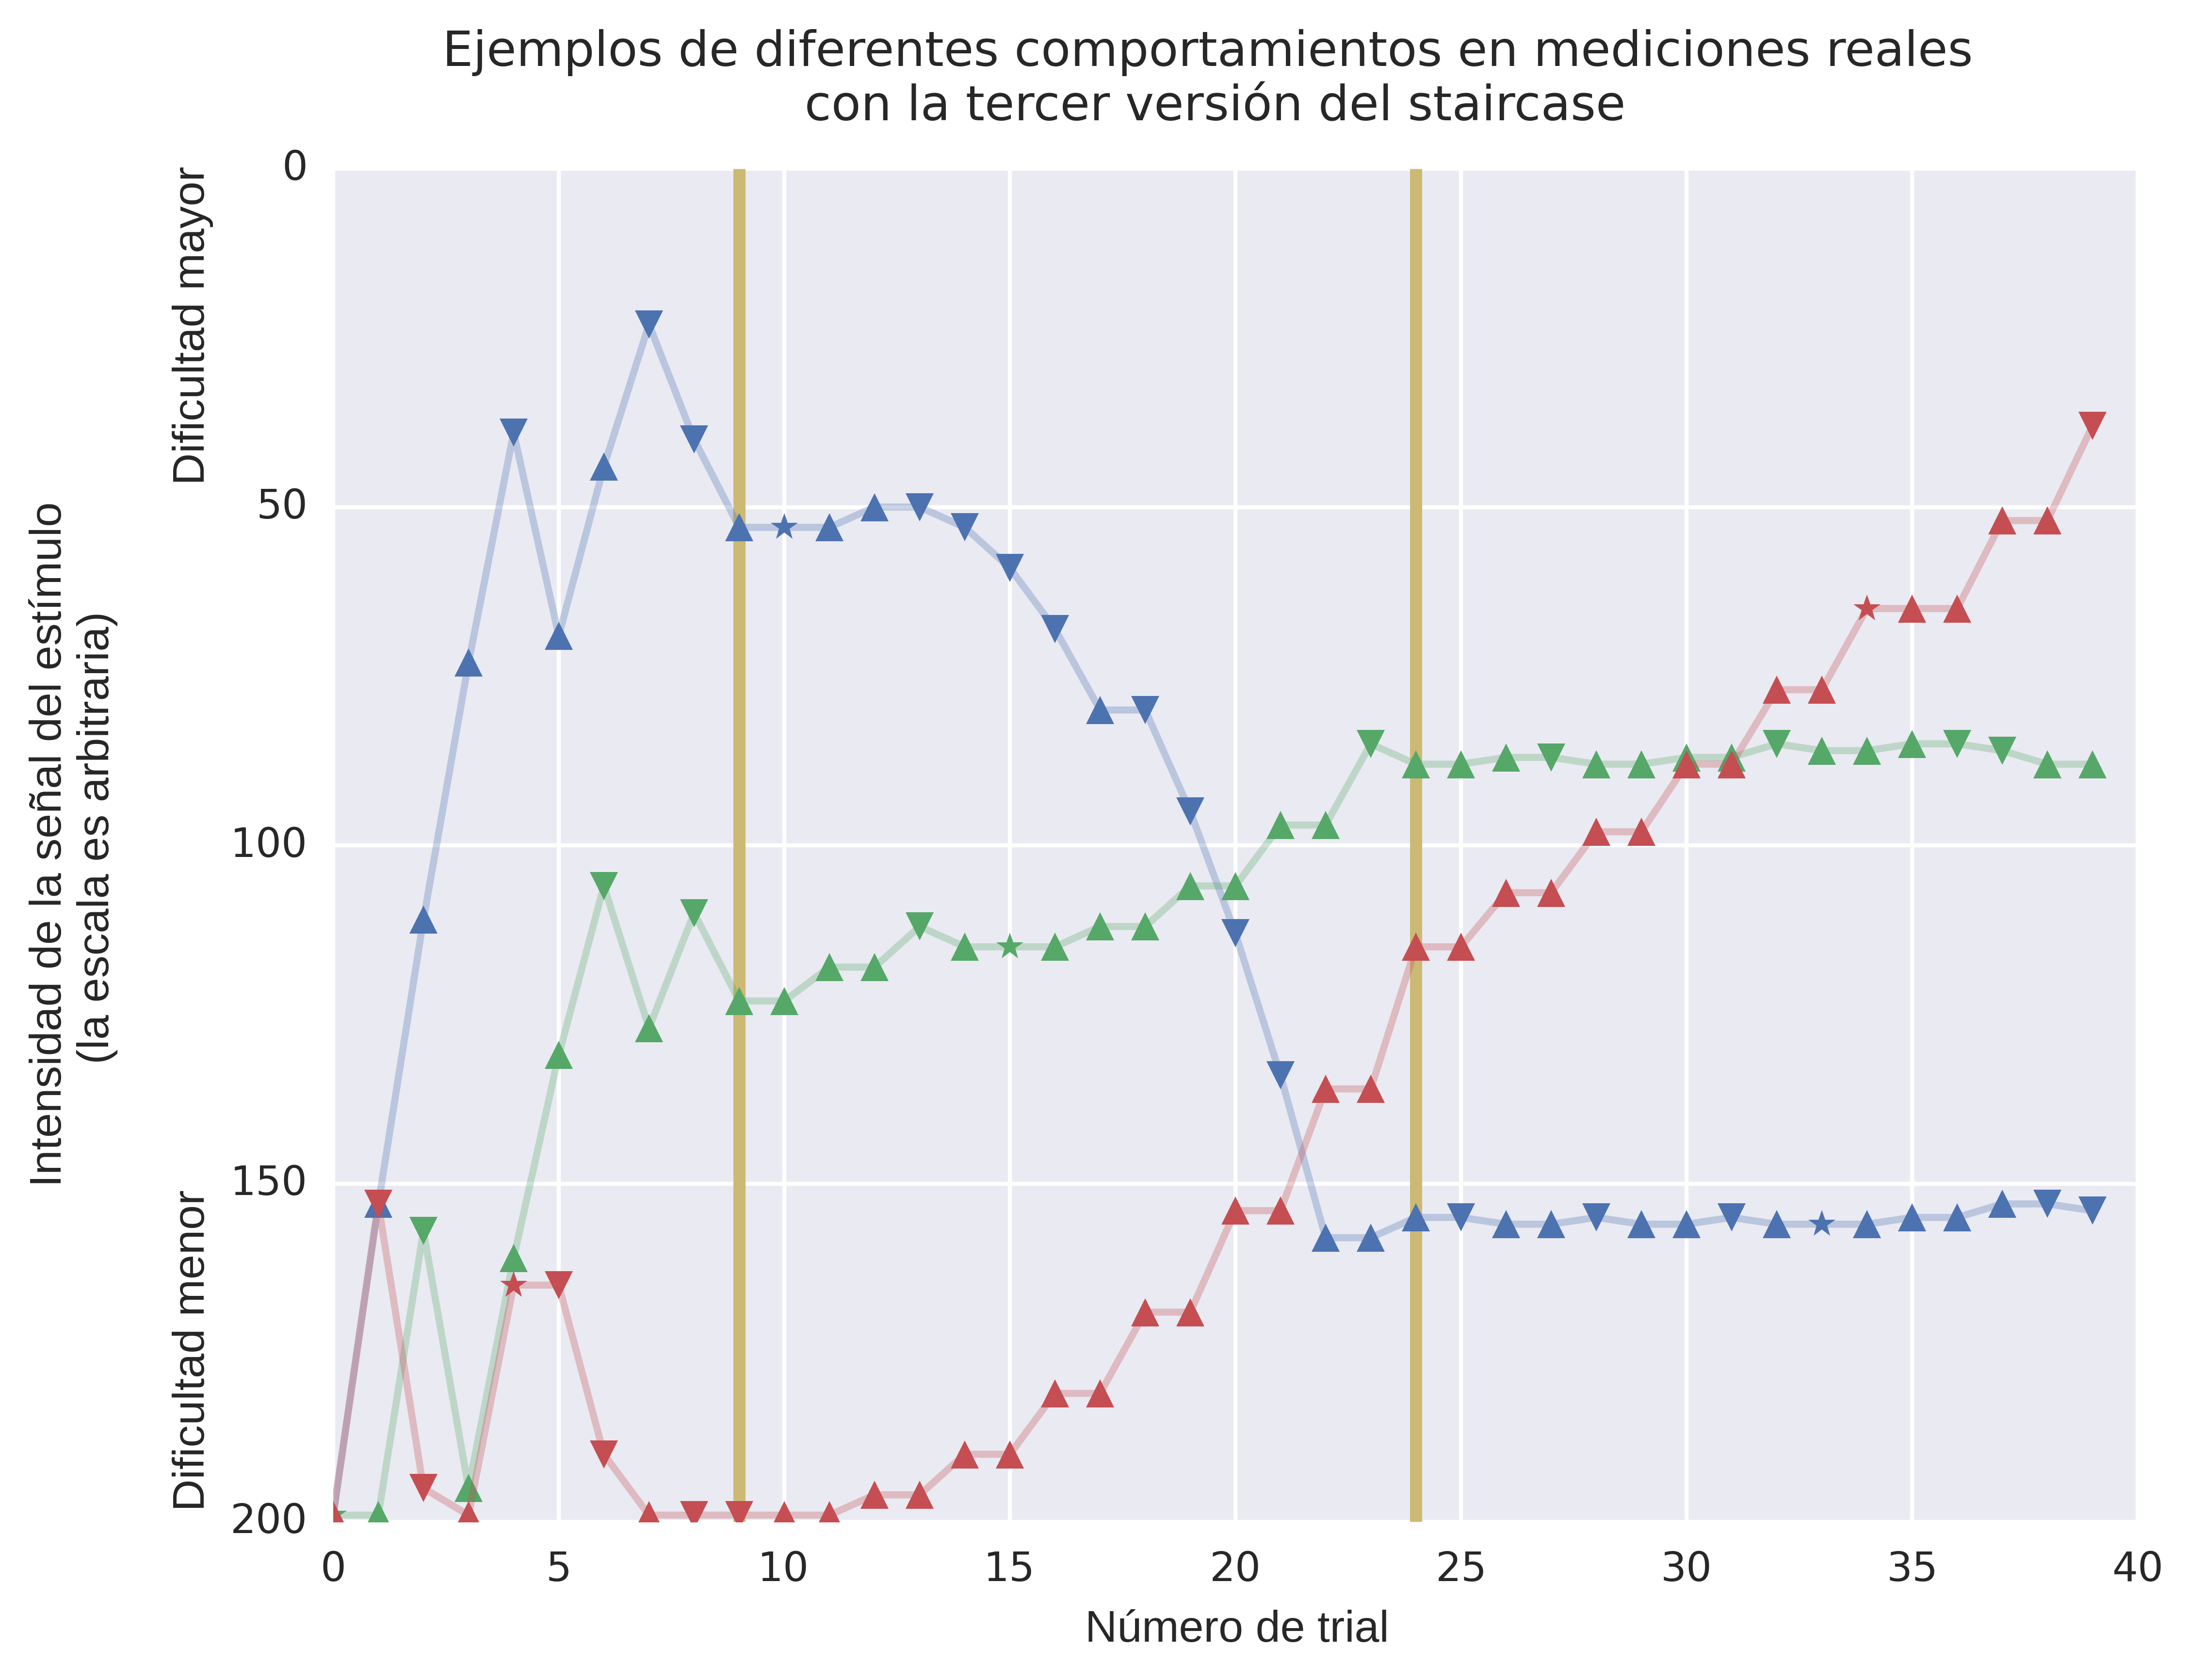
\includegraphics[width=\textwidth]{Imagenes/StairCase3.png}
        \caption{Ejemplos reales de mediciones en el experimento de entrenamiento con el algoritmo detallado en la sección \ref{staircase3}. Los CatchTrials están marcados con estrellas, y las lineas verticales delimitan las diferentes etapas del algoritmo. Como se puede observar, cuando se estabiliza, el algoritmo permite un nivel de precisión mucho mayor que en las implementaciones anteriores debido al aumento de la densidad de estimulos de señal diferente. En la figura se compara dos algoritmos que convergen correctamente con uno que no, probablemente debido a un cambio en el comportamiento del sujeto (comenzó a comprender la tarea tarde), por lo que la primer etapa finaliza en un valor muy lejano al esperado. Por su lógica, el algoritmo es mucho mas eficiente para corregir la señal si esta se excede en dificultad que si no lo hace.}
        \label{fig:staircase3}
    \end{figure}  
    
\section{Mediciones y experimentos realizados}

\subsection{Calibraciones y mediciones preliminares.} \label{resultados:preliminares}

    Como se mencionó en la sección \ref{seccion:panorama} la primer etapa del trabajo realizado consistió en un largo camino de pruebas de concepto donde evaluamos que aspectos de los que queríamos realizar eran factibles y cuales no, junto al desarrollo y perfeccionamiento de las herramientas que utilizaríamos mas adelante. 
    
    Lo primero que nos propusimos fue tener un sistema que permitiera mostrar imágenes y sus correspondientes sonidos para que los sujetos interpretaran el sistema de representación. Este trabajo llevo muchos meses donde hubo pocos resultados numéricos y la mayor parte de las pruebas las realizamos con gente del grupo de investigación o amigos cercanos. Durante este periodo desarrollamos la base funcional de la aplicación, y la adecuación del algoritmo de generación de sonidos. 
    
    Con esta base diseñamos una primer prueba en la que generamos estimulos con forma de ángulos (agudos, rectos o graves), de pares de segmentos (paralelos o no párelos) y de cuadriláteros (cuadrados, o rombos) y donde lo que buscamos fue establecer si los sujetos tenían alguna capacidad de interpretar el sistema de representación utilizado y podían distinguir entre ellas. En esta instancia las imágenes fueron generadas sin ningún tipo de algoritmo perimétrico global, sino estableciendo ciertos parámetros aleatorios en un principio y graduales posteriormente. En la figura \ref{fig:ImagenesDesarrollo1} se puede observar un ejemplo del conjunto de estimulos (y categorías) utilizados en esta fase de desarrollo. El formato de los experimentos generalmente incluía algunos trials en los que se pedía reconocer con que imagen se correspondía el sonido mostrado (de entre un conjunto de varias de ellas) o bien seleccionar entre algunas categorías conceptuales a cual correspondía el sonido. 
    
    \begin{figure}
        \center
        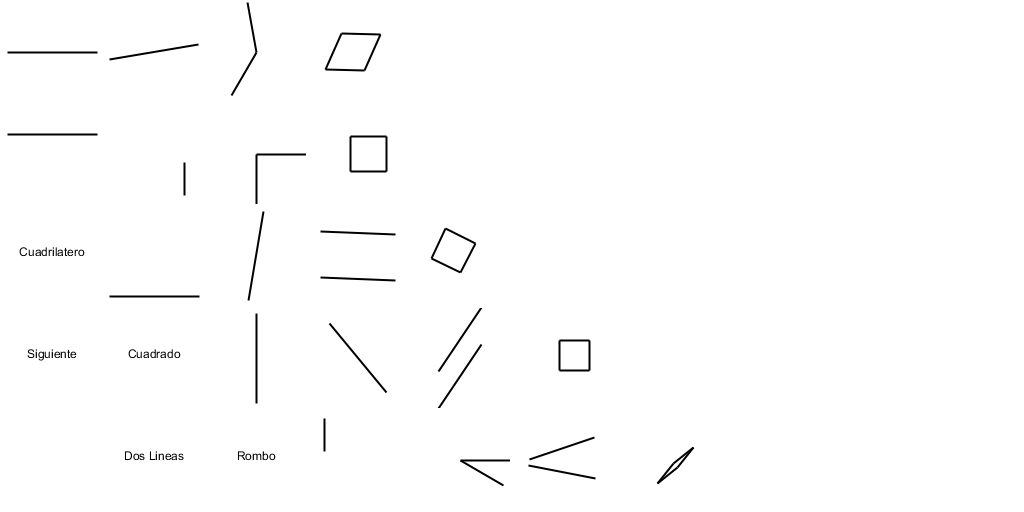
\includegraphics[width=\textwidth]{Imagenes/ImagenesDesarrollo1.png}
        \caption{Ejemplos de imágenes producidas durante la etapa inicial de prueba y calibración del dispositivo, con las que realizamos algunas mediciones preliminares para verificar que los sujetos podían distinguir entre estimulos conceptualmente muy diferentes.}
        \label{fig:ImagenesDesarrollo1}
    \end{figure}  
    
    
    \begin{figure}
        \center
        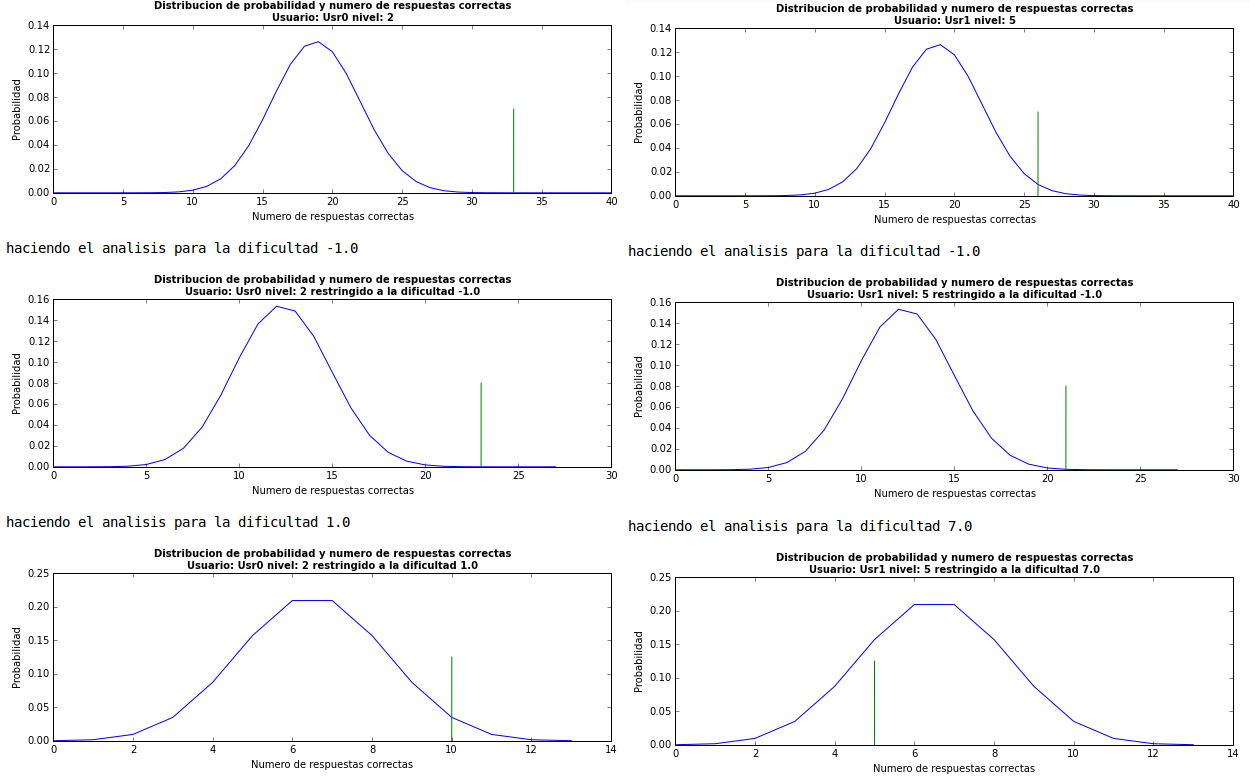
\includegraphics[width=\textwidth]{Imagenes/ResultadosIniciales1.png}
        \caption{Primeros resultados obtenidos al realizar experimentos de reconocimiento de patrones geométricos. Se mostraban estimulos muy diferentes y se debía identificar a que categoría pertenecía o cual de varias imágenes representaba. Se utilizo una primera escala de dificultad arbitraria (-1 indica que no tiene asignado valor en la escala) y se comprobó que para ciertas figuras las respuestas dadas diferían mucho de respuestas aleatorias, mientras que para otras mas complejas no. Estas mediciones sirvieron para mostrar que era necesario un mecanismo que cuantificara la dificultad de los estimulos.}
        \label{fig:ResultadosPreliminar}
    \end{figure}  
    
    Procesando los resultados obtenidos en algunos sujetos que realizaron el experimento (estas versiones se podían realizar a través de celulares fuera del laboratorio), y tras realizar la estadística correspondiente al heterogéneo espacio muestral, pudimos comprobar que las respuestas eran significativamente diferentes de respuestas generadas al azar, salvo para ciertos estimulos que a priori asumíamos muy difíciles. Ejemplo del tipo de resultados obtenidos se pueden ver en la figura \ref{fig:ResultadosPreliminar}. Con este tipo de estimulos hacer un experimento de entrenamiento carecía de sentido, ya que para entrenar y esperar un cambio en el desempeño debíamos entrenar con estímulos que no fuesen ni triviales ni imposibles. Además con estas pruebas observamos que había aspectos conceptuales que variaban fuertemente en los segmentos cercanos a los ejes cartesianos, ya que en ellos la variabilidad en los estímulos (en tanto saltos de frecuencia o duración) se acentúan.
    
    La solución que encontramos al problema fue, antes de diseñar un experimento de entrenamiento, evaluar cuanto variaba con la proximidad a los ejes la sensibilidad de los sujetos. Este fue el primer momento en que implementamos una medición tipo umbral, decisión que luego se mantuvo a lo largo de todos los demás mediciones. Nos propusimos determinar el umbral con que los sujetos podían establecer si dos recta eran paralelas o no en función de su orientación. Diseñamos para eso un setup experimental en el que mediríamos el umbral para orientaciones de -6, -3, 0, 3, 6, 10, 20, 30, 40, 50, 60, 70, 80, 84, 88, 90, 92, 94, 100, 110, 120, 130, 140, 150, 160, y 170 grados. El objetivo era poder levantar una curva de dependencia del umbral de detección con la orientación (estos ángulos completan una vuelta entera si se considera la simetría de las figuras usadas). Como resulta evidente, al ser necesarios 26 niveles, el experimento resultaba extremadamente largo. En los hechos solo lo realizamos una vez en un sujeto externo al laboratorio y otras dos sobre nosotros mismos, ya que en conjunto duraba mas de cuatro horas.  
    
    El diseño del experimento en si consistía en todos niveles equivalente donde únicamente se varió la orientación de los estimulos y el rango de valores usados en cada orientación. Para las orientaciones lejanas a los ejes se estableció los limites en 1º y 30º, en el eje horizontal entre 0.5º y 10º y en eje vertical entre 0.02º y 10º. En todos los casos se creo 50 estimulos en escala logarítmica. Para cada ángulo y orientación se construyó dos estímulos, uno que se juntara hacia un lado y otro que se juntara hacia el otro, como se puede observar en la figura \ref{fig:ImagenesDesarrollo2} donde se presentan ejemplos de los estimulos lejanos a los ejes. De esta manera el staircase descrito en la sección \ref{staircase1} disponía de dos estimulos con el mismo grado de dificultad pero orientados hacia lados diferentes y el usuario debía identificar hacia que lado estaba orientado el estimulo. Este mecanismo (junto con la aleatoricidad a la hora de seleccionar estimulos de igual dificultad) permitió que realizáramos las pruebas preliminares siendo que los sujetos conocíamos el dispositivo experimental.
    
    Durante estas pruebas comprobamos dos detalles, uno, interesante, es que el umbral de detección sonoro resulto ser mucho más sensible que el visual (al menos en las escalas gráficas utilizadas), por lo que por debajo de ciertos ángulos debíamos mostrar imágenes que no se correspondieran al nivel de señal reproducido para que el sujeto pudiera seguir eligiendo entre las direcciones de los cuadros usados como opción (ver figura \ref{fig:Pantallas2} para un ejemplo de la aplicación en funcionamiento). Por otro lado, al medir el umbral en los segmentos verticales, confirmamos que en el mejor de los casos no estaban por debajo de los 0.01º (respecto a la vertical) la capacidad de distinguir si un segmento subía o bajaba. Y esto esta muy por encima del umbral que habíamos elegido para poder representar los segmentos verticales como rampas durante la construcción de los estímulos. 
    
    En la construccion de los estímulos el $\Delta t$ mínimo se ajustó en 0.01s que en términos de pixeles (considerando la escala usada) equivale a 0.2 pixeles. Considerando que los segmentos utilizados eran del orden de los 80 pixeles de largo podemos tomar una cota inferior de 20 pixeles para la longitud de los segmentos, y considerando ángulos pequeños ($tan(\alpha)=\alpha$) nos queda que incluso dichos segmentos no podrían ser distinguidos de uno vertical. 
    
    \begin{figure}
        \center
        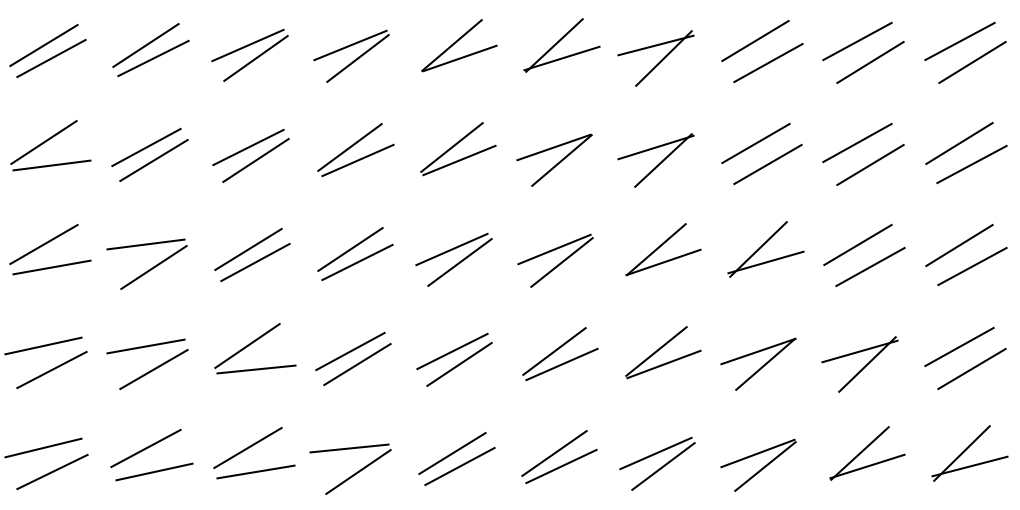
\includegraphics[width=\textwidth]{Imagenes/ImagenesDesarrollo2.png}
        \caption{Ejemplos de imágenes extraídas de las mediciones en la cual exploramos la dependencia de la sensibilidad al detectar paralelismo en función de la orientación.}
        \label{fig:ImagenesDesarrollo2}
    \end{figure}  
    
    Los resultados obtenidos para estas mediciones se pueden observar en los gráficos \ref{fig:Umbral} y \ref{fig:UmbralDetalle} donde se puede ver que cerca de los ejes efectivamente el ángulo umbral que debe haber entre dos rectas para que se detecte que no son paralelas disminuye. Dado que realizar la medición con muchos sujetos en forma correcta para poder extraer conclusiones era imposibles por el tiempo que réqueria el diseño experimental planteado, el siguiente paso fue realizar una medición adecuada, con un diseño experimental realizable, que validara los resultados obtenidos hasta el momento.
    
    \begin{figure}
        \center
        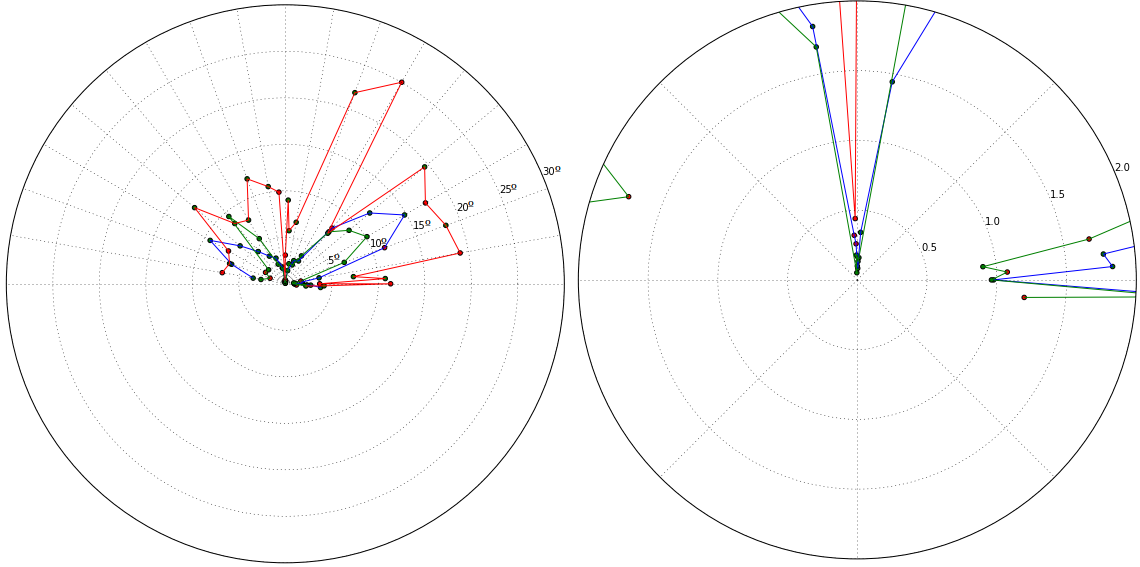
\includegraphics[width=\textwidth]{Imagenes/Umbral.png}
        \caption{En esta figura se muestran las mediciones preliminares donde se busco caracterizar la dependencia con la orientación del mínimo ángulo que debe haber entre dos rectas para que se pueda distinguir que no son paralelas. Se realizo dos pruebas en un mismo sujeto miembro del laboratorio que conocía el diseño experimental y estaba acostumbrado a escuchar estos estímulos, y una medición con un sujeto externo (la medición en rojo). A la derecha se muestra los resultados usando una escala completa, en un gráfico radial donde en cada dirección se marca el ángulo mínimo necesario para detectar el no paralelismo. A la izquierda se muestra los mismos resultados ampliando la escala para visualizar el efecto en los ejes.}
        \label{fig:Umbral}
    \end{figure}  
    
    
          
    \begin{figure}
        \center
        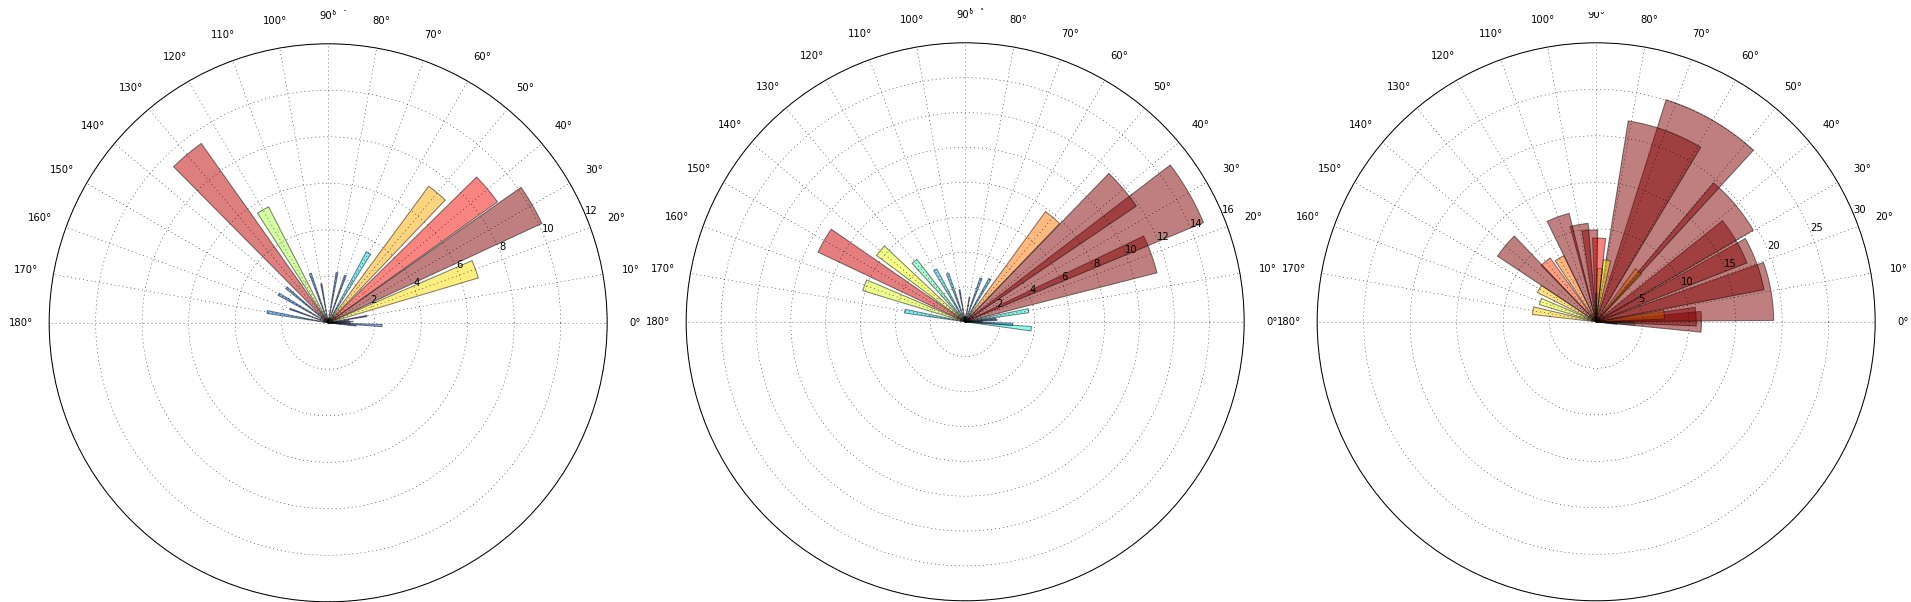
\includegraphics[width=\textwidth]{Imagenes/UmbralDetalle.png}
        \caption{Detalle de la figura \ref{fig:Umbral} donde se representa en otro formato la misma información separando por sujeto. El sujeto de la derecha es el único que no estaba acostumbrado de antemano a la tarea. En todos las mediciones el orden de realización de los niveles fue variando la orientación en en sentido antihorario.}
        \label{fig:UmbralDetalle}
    \end{figure}  
    
    
    Sin embargo de estas pruebas se puede observar que la sensibilidad (definida como la inversa del umbral) aumenta mucho en los ejes (los mismo sabíamos que sucedía para pruebas en ángulos aunque no hubiéramos realizado pruebas exhaustivas). Mas allá de no disponer de datos adecuados para realizar un ajuste, se puede interpretar este hecho en posibles alternativas de como los sujetos disciernen los estímulos, que sean compatibles con los datos observados. 
    
    Si consideramos que lo que se puede cuantificar con la percepción es la variación de frecuencias $\Delta f$ (siempre en escala logarítmica que es como esta representado todo el sistema) que corresponde a cada segmento así como su duración $\Delta t$, cabe preguntarse como se puede distinguir la orientación de los segmentos con esta información. Considerando un segmento de largo arbitrario L (el argumento utilizado vale independientemente de la posición y tamaño del segmento dentro del lienzo), dichas variaciones quedan dadas por las ecuaciones \ref{ec:DeltaT} y \ref{ec:DeltaF} que no son mas que las proyecciones del segmento sobre los ejes.
    
    Sin embargo para poder discernir los estimulos no alcanza con cuantificar estas magnitudes en abstracto sino que deben ser comparadas con algún patrón. Surgen entonces diferentes opciones: que los estimulos sean identificados comparando ambos aspectos para el mismo segmento o bien contra otro segmento (ya sea un recuerdo de lo esperado o el otro existente en la figura). Debido al sistema de representación, en ambos casos el resultado que se obtiene es similar. 
    
    En caso de que se comparen ambas variables del mismo segmento, una va como el $cos(\alpha)$ y la otra como $sin(\alpha)$, por lo tanto cerca de los ejes, una de los dos se hace máxima y la otra se aproxima a cero. Al compararlas (dividirlas), la expresión de este resultado queda proporcional a $tan (\alpha)^{\pm1}$ que diverge en los ejes y es mínima en 45º. Obviamente como es imposible percibir $\Delta t$ y $\Delta f$ con infinita resolución la sensibilidad tiene un limite finito. 
    
    Otra interpretación posible es que en proceso de detectar cambios en la orientación se compare el resultado detectado contra el esperado en la orientación a detectar. Aquí, nuevamente queda como expresión de sensibilidad algo proporcional a $tan (\alpha)^{\pm1}$ ya que se esta comparando una función que tiene forma trigonométrica, con su deriva. Esto aplica tanto a la tarea de determinar si un segmento esta orientado cerca o lejos de los ejes (para la tarea de reconocer ángulos donde el lado fijo esta sobre un eje), como para la tarea de reconocer si dos segmentos son paralelos o no. 
    
    
    \begin{equation} \label{ec:DeltaF}
        \Delta f = A \cdot L \cdot sin (\alpha)
    \end{equation}
        
    \begin{equation} \label{ec:DeltaT}
        \Delta t = B \cdot L \cdot cos (\alpha)
    \end{equation}

    \subsection{Medición del umbral de percepción en función de la orientación} \label{seccion:Exp1}
    
    \subsubsection{Diseño y métodos}
    
    El objetivo de este experimento fue observar en forma adecuada y experimentalmente valida datos que ratificaran los resultados preliminares. A su vez serviría como prueba de concepto para poner a punto la implementación de un experimento realizado en ambiente controlado de laboratorio.
    
    Para esto, y con el antecedente de que las pruebas preliminares eran extremadamente largas, se seleccionó un subconjunto reducido de orientaciones (0º, 30º y 90º) donde se buscó realizar una evaluación muy similar a la ya implementada. Además en las mismas orientaciones se incluyó una medición equivalente para la capacidad de distinguir ángulos. 
    
    Para cada orientación se generó dos secuencia de 40 estimulos en el caso de paralelismo, donde la separación angulas entre ambos segmentos vario de 0.1º a 25º en escala logarítmica. En cada orientación se generaron estimulos que convergieran hacia uno u otro lado (denominadas 'convergencia positiva' y 'convergencia negativa'. Cada serie de estimulos fue asignada a un algoritmo StairCase como el que se describe en la sección \ref{staircase2}. 
    
    En el caso de los ángulos primero se generó todo el conjunto de estimulos posibles creando ángulos con un lado (denominado 'fijo') orientado en 0º, 30º, y 90º y el otro orientado de a saltos de 10º, donde se incluyó un aumento de la densidad (saltos de 2º) en los ángulos que estaban alrededor de los ejes (en un rango de $\pm$ 10º). Una vez creados todos estos estimulos se seleccionó para cada orientación los que formaran ángulos de entre 9º y 90º grados para asignarlos a lo que denominamos 'dinámica aguda' y los que formaran ángulos de entre 90º y 171º para asignarlos a la denominada dinámica obtusa'. Cada una de estas series (que no incluyen siempre la misma cantidad de estímulos diferentes) se asignó a un StairCase. 
    
    \begin{figure}
        \center
        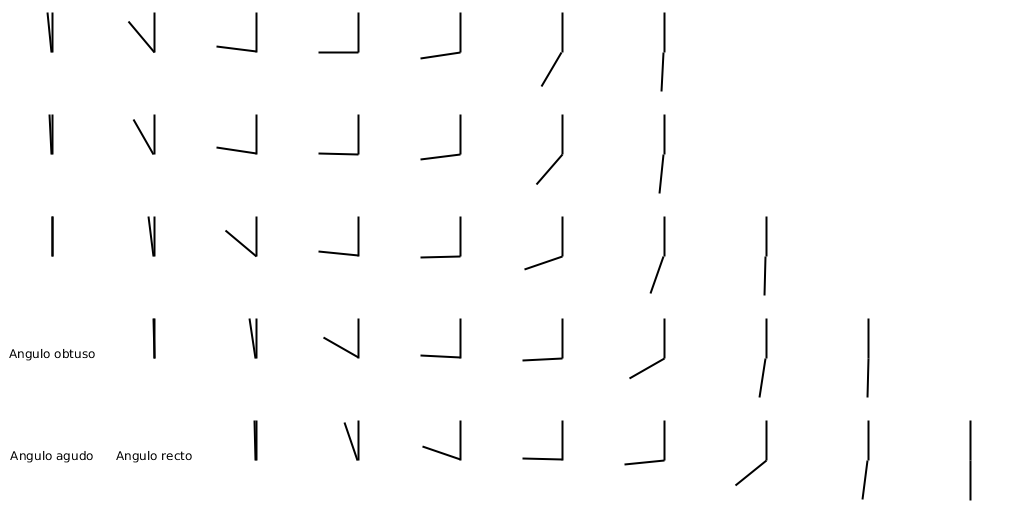
\includegraphics[width=\textwidth]{Imagenes/ImagenesExp1_2.png}
        \caption{Ejemplo de estímulos utilizados durante el experimento de medición de umbral en función de la orientación (para el caso 90º). Técnicamente estos estimulos nunca son mostrados al sujetos en forma visual sino en su representación sonora (con excepción de los tres cuadros de texto). No todos los estímulos son mostrados por el algoritmo.}
        \label{fig:ImagenesExp1}
    \end{figure}  
    
    Para la realización del experimento se convocó a doce sujetos del ámbito universitario (tanto de la UBA, como de la Universidad Torcuato Di Tella) que concurrieron entre una única vez entre el 30 de Marzo de 2015 y el 14 de Abril de 2015 al Laboratorio de Neurociencia de la Universidad Torcuato Di Tella. A todos los sujetos se les explicó las tareas a desarrollar y se les pidió que firmaran el consentimiento de participar en el experimento que estuvo enmarcado en el protocolo aprobado por el comité de ética del Cemic. 
    
    El experimento fue realizado en un cuarto vació y aislado de posibles perturbaciones sonoras y atencionales disponible para este tipo de experimentos. El software utilizado se ejecuto sobre una laptop disponible a tal efecto que contaba con un mouse y auriculares (externos, no in-ear). En caso de que los sujetos prefirieran se les ofrecía utilizar auriculares propios con los que se sintieran más a gusto.
    
    Como protocolo de realización del experimento, se les presentaba a los sujetos el marco en que el experimento se estaba desarrollando, sus objetivos y la lógica de representación del Visound, también se les hacia explicito el objetivo detrás de la tarea a realizar. La sesión fue diseñada con nueve niveles. Los tres primeros a modo de tutorial donde nos quedábamos en compañía de los sujetos hasta verificar que estuvieran comprendiendo la tarea a realizar, luego nos retirábamos y el sujeto avisaba al concluir los niveles. 
    
    De los tres niveles de tutorial, el primero constaba de una sucesión de pantallas en la que se mostraban figuras sencillas y se podía escuchar su correspondiente representación sonora. La idea de este nivel fue consolidar lo explicado verbalmente en la presentación del experimento. También en este nivel se sugería a los sujetos utilizar un control de volumen (incluido dentro de la aplicación) para que pudieran escuchar bien todos el rango de frecuencias (los graves suelen escucharse peor que los agudos). El segundo y tercer nivel fueron niveles de ejemplo del funcionamiento del programa donde se armó un nivel muy corto (10 trials) de paralelismo y ángulos equivalente en todo a los que tendrían que realiza luego excepto en la orientación (180º para ángulos y 10º para paralelismo) y en que este nivel tutorial devolvía feedback para que los sujetos pudieran saber si estaban interpretando bien o no la tarea. 
    
    \subsubsection{Resultados obtenidos}
    
    \begin{figure}
        \center
        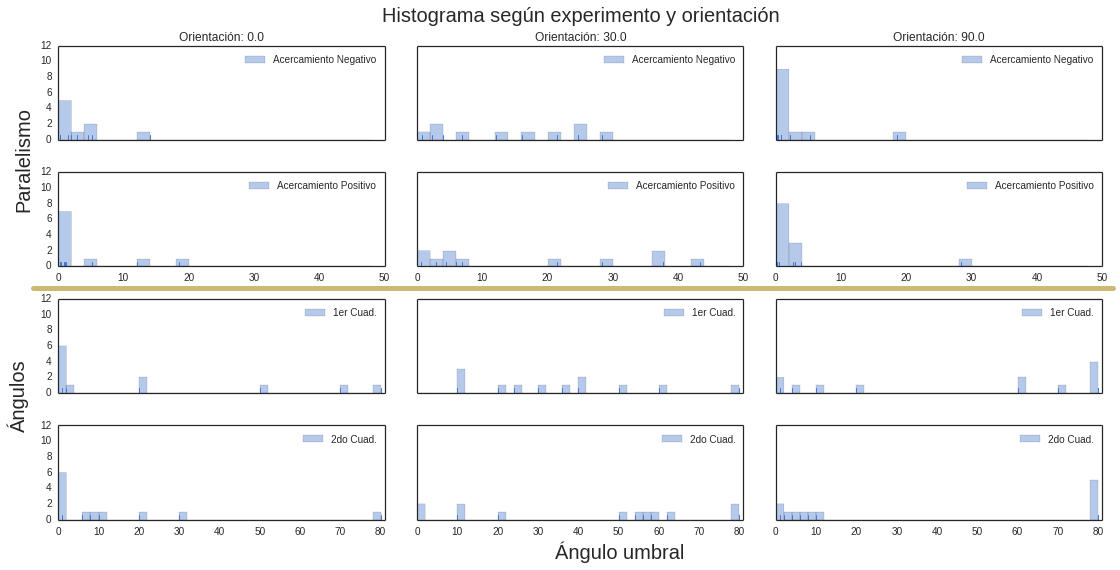
\includegraphics[width=\textwidth]{Imagenes/Exp1_DataCruda.png}
        \caption{En la figura se puede observar la información recolectada durante el experimento de medición de umbral de detección en función de la orientación. Hubo seis experimentos simultáneos (tres orientaciones y dos categorías) donde para cada experimento y sujeto se tomar dos mediciones correspondientes a la capacidad de distinguir categorías con estímulos que diferían del neutro en forma complementaria.}
        \label{fig:Exp1DataCruda}
    \end{figure}  
    
    En la figura \ref{fig:Exp1DataCruda} se puede observar el resultado de cada una de las mediciones realizadas a cada uno de los 12 sujetos en forma de histograma. A primera vista se puede observar que en el caso de la orientación que no esta en el eje, la distribución esta mucho mas lejos de los ejes, mientras que en 0º y 90º se observa efectos de saturación sobre los ejes. Por otro lado se observa una elevada cantidad de mediciones que saturan en el rango para la orientación de 90º en ángulos. En cambio no hay prácticamente sujetos que en paralelismo hayan saturado en el umbral máximo. Pero todos estos resultados deben ser validados considerando que el algoritmo de StairCase puede estar fallando. 
    
    El efecto de que muchos sujetos hayan reportado un umbral en 81º para los experimentos de ángulos a 90º no es algo inesperado, ya que que refleja una hipótesis considerada durante los estudios preliminares y que tuvimos la oportunidad de evaluar con este experimento. Si se observa en el ejemplo de estímulos de la figura \ref{fig:ImagenesExp1}, que es la que se corresponde con esta orientación, los estímulos a discernir incluyen un lado de referencia que esta vertical, y en pruebas anteriores habíamos descubierto que los segmentos verticales (que suenan como un chasquido rápido) son difíciles de ubicar en altura. Los sujetos al realizar este experimento sabían que los ángulos mostrados se construían en forma de agujas del reloj, por lo tanto un segmento vertical podía estar en la mitad superior o inferior de la pantalla. Y por la simetría de los estímulos, si los sujetos ubicaban el segmento en la mitad equivocada, todo lo que interpretaran como ángulo obtuso seria agudo y viceversa. Esta interpretación fuerza al algoritmo a mantener la señal en su valor inicial elevado (por lo que el sujeto sigue escuchando estímulos muy fáciles) y luego de seis respuestas incorrectas se detiene. 
    
    \begin{figure}
        \center
        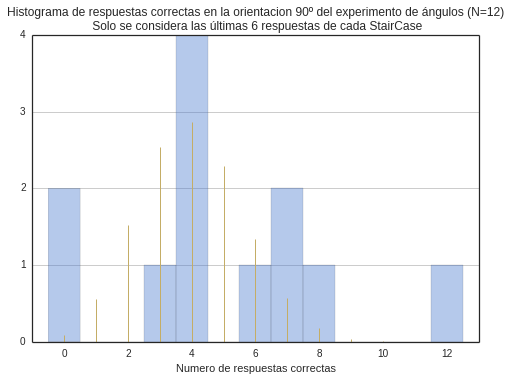
\includegraphics[width=\textwidth]{Imagenes/Exp1_Saturacion.png}
        \caption{Se compara el histograma de numero de respuestas correctas obtenidas por cada sujeto durante los últimos seis trials de cada StairCase en el experimento de ángulos a 90º, con la probabilidad de tener dicho numero de respuestas (lineas finas amarillas) correctas si los sujetos respondieran al azar. Los dos sujetos que respondieron todas mal tienen una probabilidad de 0.0924 de haber obtenido ese resultado al azar, por lo que la probabilidad conjunta es menor a 0.009. Este resultado estadisticamente muy improbable lo adjudicamos a que interpretan incorrectamente la posición del lado que no se mueve en los diferentes estímulos (ver figura \ref{fig:ImagenesExp1}). Este el único caso de todas las orientaciones posibles donde se observó el efecto, lo que se condice con la hipótesis planteada.}
        \label{fig:Exp1Saturacion}
    \end{figure}  
    
    Para evaluar la hipótesis mencionada lo que realizamos fue una comparación entre el numero de respuestas que dio cada sujeto contra lo esperado en la hipótesis de que los sujetos respondieran al azar. El resultado se puede ver en la figura \ref{fig:Exp1Saturacion} donde se observa las dos series de respuestas correspondientes a los dos StairCase que se ejecutan en cada nivel mezcladas, hay dos sujetos cuyo mal desempeño tiene muy poca probabilidad de ser producto del azar, para el calculo comparamos contra la distribución de respuestas aleatorias pesando por el numero de muestra tomadas (corrección de Bonferroni) y luego calculamos la probabilidad conjunta de que dos sujetos hayan tenido tan mal desempeño. Al ser la probabilidad de este evento inferior a 0.009, es razonable suponer que hay algún sesgo en las respuestas incorrectas detrás del resultado. Y dado que de todas las orientaciones posibles esta es la única en la que se observaron desempeños marcadamente peores que los producto del azar, podemos suponer que el evento refleja la hipótesis de que la altura de un segmento vertical es difícil de determinar en el contexto estudiado.
    
    También para poder distinguir los casos en los que los sujetos actuaron comprendiendo la tarea (y por ende tiene sentido decir que la medición realizada representa la percepción del sujeto) de los casos en los que los sujetos respondieron al azar, realizamos un análisis similar pero distinguiendo los sujetos que en el conjunto de las pruebas correspondientes a cada nivel (considerando los dos StairCase como una serie de respuestas) respondieron mejor que si se tratara de respuesta al azar. Para este análisis consideramos el hecho de que los diferentes sujetos reportaron diferente numero de respuestas (pues el StairCase diseñado puede finalizar el nivel antes de las 40 pruebas) y de que cada tipo de experimento (ángulos/paralelismo) tenia un chance diferente al responder al azar. Tomamos como criterio para distinguir, que muestras son validas y cuales no, si la muestra correspondiente a cada nivel por separado tenia probabilidad menor al 0.05 de ser una respuesta producto del azar. 
    
    En la figura \ref{fig:histoTrialsxNivel} puede visualizarse que la mayoría de los niveles concluyo en 40 trials, y que pocos de ellos se pueden atribuir al azar. Un ejemplo gráfico del análisis realizado para distinguir muestras validas de invalidas se puede ver en la figura \ref{fig:Exp1_Significancia}
	
	\begin{figure}
        \center
        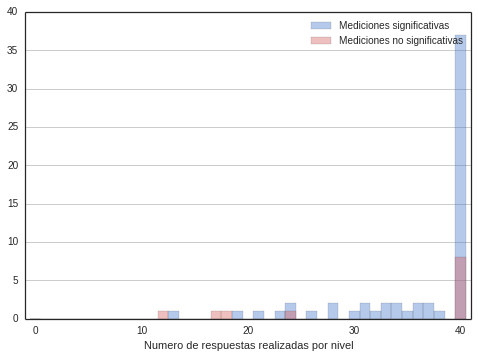
\includegraphics[width=0.8\textwidth]{Imagenes/Exp1_NroRespuestas.png}
        \caption{Histograma de numero de respuestas medidas por nivel (en total hay 72 niveles realizados). El numero esperado era 40, pero algunos niveles concluyeron con menos trials porque ambos StairCase (descriptos en la sección \ref{staircase2}) finalizaron antes. En color azul se indican los niveles cuyas mediciones superaron un test de signifícancia comparando contra respuestas al azar, en rojo los que nos.}
        \label{fig:histoTrialsxNivel}
    \end{figure}  
	
	
	\begin{figure}
        \begin{subfigure}{.5\textwidth}
            \centering
            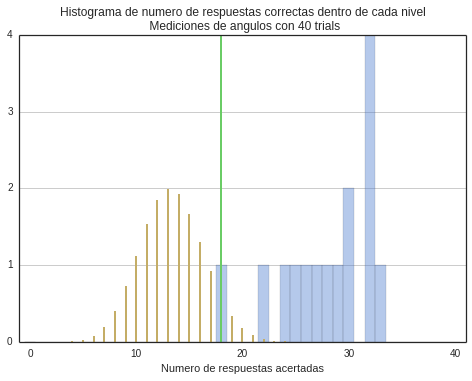
\includegraphics[width=\textwidth]{Imagenes/Exp1_Validas40A.png}
            \caption{Resultados para las mediciones de ángulos donde la chance es un tercio}
            \label{fig:sfig1}
        \end{subfigure}
        \begin{subfigure}{.5\textwidth}
            \centering
            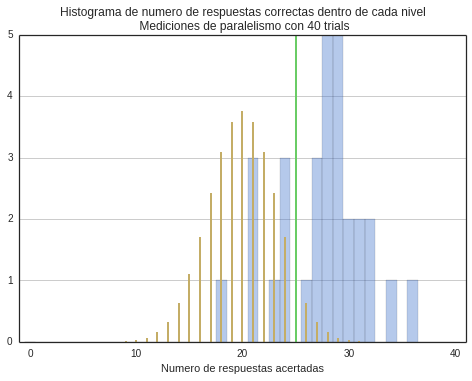
\includegraphics[width=\textwidth]{Imagenes/Exp1_Validas40P.png}
            \caption{Resultados para las mediciones de paralelismo donde la chance es un medio}
            \label{fig:sfig2}
        \end{subfigure}
        \caption{Figura donde se compara el histograma de respuestas correctas con la distribución esperada para cada tipo de experimento si se realizaran respuestas al azar. La linea vertical en verde indica a partir de que valores hay una probabilidad significativa ($pValue<0.05$) de que cada muestra no sea producto del azar. Se realizo el gráfico solo con el subconjunto de datos de 40 respuestas porque al variar este parámetro se modifica la distribución y como se puede observar en la figura \ref{fig:histoTrialsxNivel} este fue el valor que más muestras incluye}
        \label{fig:Exp1_Significancia}
    \end{figure}

    Habiendo realizado este análisis, lo que nos propusimos fue comparar entre las muestras validas, como cambia el umbral de detección en función de la orientación. Los resultados pueden verse en la figura \ref{fig:Exp1Resultados} donde nos encontramos con el problema de, producto del descarte de datos, no todas las mediciones provienen del mismo conjunto de sujetos, ni resulta evidente que las tendencias observadas sean significativas. Un punto interesante a destacar de este resultados es que hay muchas menos muestras descartadas en los experimentos de ángulos que en los de paralelismo, pese a que se observa que es una tarea mas difícil. De hecho los únicos dos datos descartados se corresponden con los dos que respondieron sistemáticamente mal en el gráfico \ref{fig:Exp1Saturacion}. 
    
    Una posible explicación para este efecto es que el StairCase utilizado da saltos mas grandes al inicio que al final, por lo que si un sujeto reconoce sistematicamente bien los estímulos fáciles converge rápidamente a la zona donde se busca que no pueda responder bien (es decir que se fuerza al sujeto a responder con chance aproximadamente un tercio), lo cual empeora su estadística. En cambio si un sujeto tarda en comenzar a responder bien porque le cuesta acostumbrarse a la tarea, el StairCase mostrar una aproximación tardía y lenta al umbral, lo que se corresponde con un elevado numero de respuestas correctas. Además, observamos que al tener la escala utilizada en los ángulos un paso más grande y ser el estímulo recto marcadamente diferente a los demás (en orientación 0º y 90º), en algunos casos los sujetos saturaron la escala en reconocer bien el estimulo (que por lo tanto se repite, como se ve en el ejemplo marcado en azul en la figura \ref{fig:staircase2}), cosa que no puede suceder en los experimentos de paralelismo. Ambos efectos combinados puede explicar porque hay tanta diferencia en el numero de muestras descartadas. 
    
    \begin{figure}
        \center
        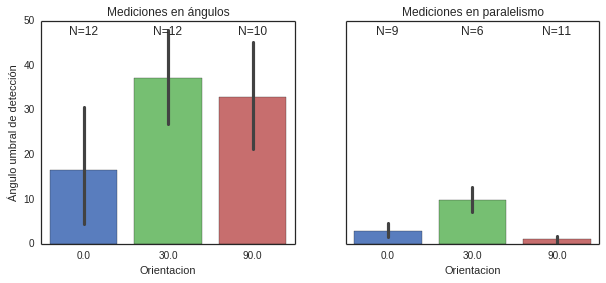
\includegraphics[width=\textwidth]{Imagenes/Exp1_Resultados.png}
        \caption{Resultados obtenidos para la medición de umbral en las diferentes orientaciones y categorías. Si bien se observa una tendencia a que en los ejes el umbral sea menor, los resultados no son comparables porque pertenecen a un subconjunto diferente de los sujetos en cada orientación. En la figura \ref{fig:Exp1_ResultadosDetalle} se realiza el correspondiente análisis estadístico entre las submuestras comparables de este conjunto.}
        \label{fig:Exp1Resultados}
    \end{figure}  
	
	\begin{figure}
        \center
        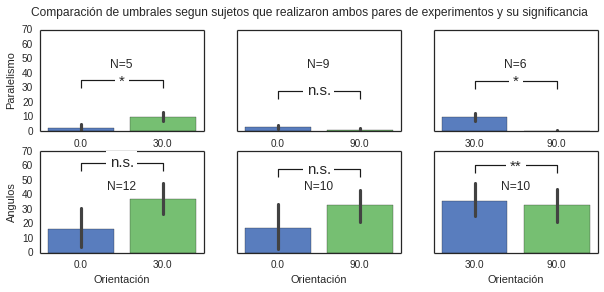
\includegraphics[width=\textwidth]{Imagenes/Exp1_ResultadosDetalle.png}
        \caption{Comparación entre los umbrales detectados por los sujetos según las diferentes orientaciones y categorías a las que pertenecían. En cada caso se comparó sólo muestras en donde los resultados pertenecieran a sujetos que realizaron ambas pruebas superado un test que permitiera asumir que no estaban respondiendo al azar. Esto se hizo para que que el test pudiera realizarse sobre muestras relacionadas.}
        \label{fig:Exp1_ResultadosDetalle}
    \end{figure}  
    
    En la figura \ref{fig:Exp1_ResultadosDetalle} se puede observar la comparación final entre todos los datos estadísticamente comparables. Se puede observar que la única orientación que muestra diferencias significativas con las demás es la de 30º, y que como se esperaba cuando las orientaciones de los segmentos están alejados de los ejes cartesianos la capacidad de distinguir entre las orientaciones de los segmentos disminuye. 
    
    
    \subsection{Medición del efecto del entrenamiento en la mejora del umbral}
    
    \subsubsection{Diseño y métodos} \label{seccion:Exp2_Diseno}
    
    El objetivo de este experimento fue evaluar el efecto del entrenamiento en la capacidad de percepción de las categorías geométricas de paralelismo y ángulo recto. Se eligió realizar pruebas con formato similar al experimento anterior, pero mejorando el algoritmo de StairCase (ver sección \ref{staircase3}) y eligiendo orientaciones lejanas a los ejes para maximizar el posible efecto de mejora evitando saturar la medición. En todas las mediciones (o niveles) se propuso medir el umbral de detección como medida a comparar.
    
    Se eligió realizar pruebas de medición del umbral de detección en orientaciones de 30º, 60º, 120º y 150º en las categorías de ángulos y paralelismo. La elección de las orientaciones se realizó porque estas orientaciones combinadas con la construcción de los estímulos utilizados presentan un alto nivel de simetrías, tanto de rotación como de reflexión (ver figuras \ref{fig:simetrias}). Como protocolo para observar el efecto del entrenamiento se decidió realizar una evaluación inicial a todos los sujetos en todas las orientaciones propuestas, luego entrenar a algunos de ellos en una orientación especifica, y volver a realizar una evaluación en todas las orientaciones iniciales. 
    
    \begin{figure}
        \begin{subfigure}{.47\textwidth}
            \centering
            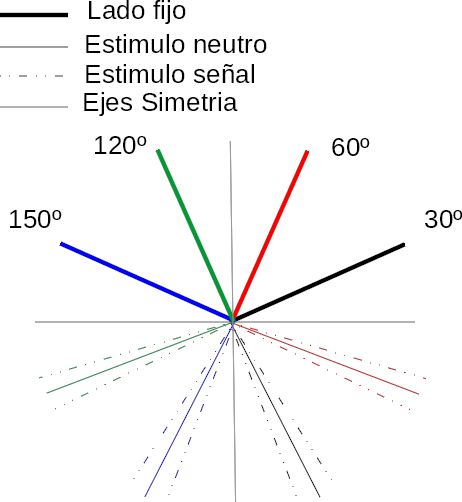
\includegraphics[width=\textwidth]{Imagenes/SimetriasOrientacionAngulos.png}
            \caption{Simetrias presentes en los estímulos utilizados para las evaluaciones de percepción en ángulos.}
        \end{subfigure}
        \begin{subfigure}{.53\textwidth}
            \centering
            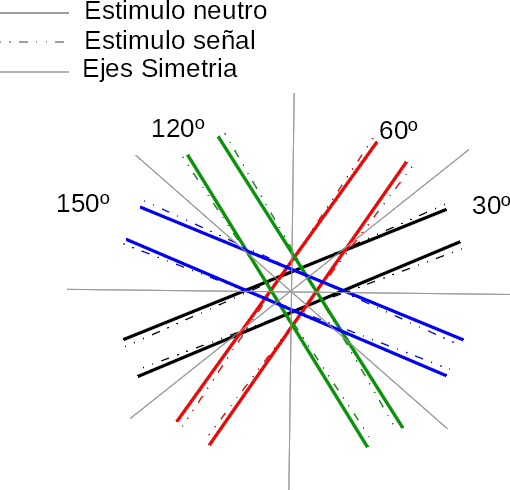
\includegraphics[width=\textwidth]{Imagenes/SimetriasOrientacionParalelismo.png}
            \caption{Simetrias presentes en los estímulos utilizados para las evaluaciones de percepción en paralelismo}
        \end{subfigure}
        \caption{Para realizar el experimento de entrenamiento se utilizaron estímulos con un alto nivel de simetría, de manera de poder observar posibles efectos de transferencia entre las diferentes transformaciones de simetría luego de entrenar en una orientación específica.}
        \label{fig:simetrias}
    \end{figure}

    A diferencia del experimento anterior, en cada orientación se generó una amplia variabilidad de estímulos, utilizando como parámetro de variabilidad pequeñas rotaciones además de las variaciones en la intensidad de la señal necesaria para la lógica del StairCase. Esta decisión estuvo basada en otro cambio que realizamos en la lógica del StairCase (ver sección \ref{staircase3}) y del diseño experimental que fue preguntar en cada estímulo explícitamente por las categorías paralelo/no paralelo y recto/no recto en lugar de preguntar hacia que 'lado' apunta el estímulo. De esta manera necesitabamos intercalar estímulos neutros entre los estímulos con señal por lo que debía haber muchos estímulos neutros similares pero no idénticos. La solución a esto fue generar un estimulo neutro en la orientación deseada y pequeñas rotaciones del mismo. A priori esto rompe la condición de que la medición sea en una orientación precisa, pero dado que no es el objetivo ver la dependencia con la orientación, y las orientaciones pensadas difieren mucho mas que las pequeñas rotaciones propuestas no consideramos que esto sea un problema. Dado que realizamos pequeñas rotaciones en los estímulos neutros, también lo hicimos en los estímulos con señal.
    
    En los estímulos de paralelismo, para cada orientación, se generaron 200 estímulos distribuidos linealmente en su intensidad entre los 0.1º y 100º. A su vez se crearon cinco rotaciones de cada uno de estos estímulos en 0º, $\pm$2.5º y $\pm$5º. Del estímulo neutro se generaron 20 rotaciones entre 10º y -10º (Como se puede ver en la figura \ref{fig:ImagenesExp2}). Para los ángulos se crearon las mismas fluctuaciones pero los estímulos variaron entre 1º y 80º. Además se crearon dos series más cortas en 180º y 0º para los tutoriales de ángulos y paralelismo. 
    
    La estructura de niveles se configuró en 40 estímulos por nivel para las evaluaciones iniciales y finales sin feedback. El entrenamiento se diseño como una secuencia de tres niveles uno con feedback de 100 estímulos, uno de 50 estímulos sin feedback, y uno final igual al inicial. Esta secuencia se repitió en cuatro sesiones (realizadas en días diferentes) con las orientaciones de 30º ya sea de ángulos o paralelismo. En el caso del entrenamiento el segundo y tercer nivel iniciaban es StairCase en el nivel de señal que concluyo el inmediato anterior. 
    
    Todo el protocolo experimental por el cual se convocó a sujetos, y se les explicó la tarea a realizar fue idéntico al mencionado en el experimento anterior con la diferencia de que tras la primer sesión (día de experimento) los sujetos simplemente concurrían al laboratorio y comenzaban con las mediciones. Además en este caso se les ofreció a los sujetos una recompensa económica al finalizar todas las sesiones de medición.
    
    \begin{figure}
        \center
        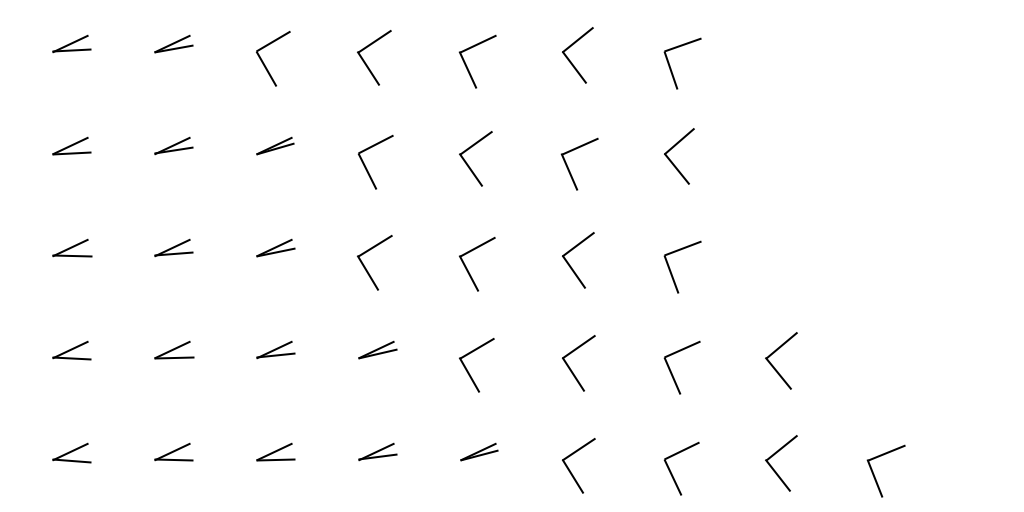
\includegraphics[width=\textwidth]{Imagenes/ImagenesExp2.png}
        \caption{Ejemplo de parte de los estímulos utilizados para el último experimento en la orientación 30º de ángulos. Se observa que hay 21 estímulos neutros rotados alrededor de la orientación media, y una mayor densidad de estímulos en comparación con el experimento anterior (figura \ref{fig:ImagenesExp1}).}
        \label{fig:ImagenesExp2}
    \end{figure}  
    
    \subsubsection{Resultados obtenidos}
    
    Con el procedimiento experimental mencionado concurrieron diez sujetos al laboratorio. Cinco de ellos realizaron el proceso de entrenamiento (tres en paralelismo y dos en ángulos), los otros cinco realizaron las mediciones de control. El limitado numero de sujetos que concurrió se debió a la dificultad de conseguir personas que estuvieran dispuestas a participar de seis sesiones diferentes con disponibilidad horaria suficiente como para que las mediciones no duraran mas de tres semanas, combinado con que los resultados preliminares mostraron ser diferentes a lo que habíamos esperado al construir el diseño del experimento . Por esta razón decidimos concluir el experimento con este limitado número de sujetos para analizar los resultados obtenidos hasta el momento.
    
    Los datos medidos se pueden visualizar (previo a cualquier filtro o análisis de datos) en las figuras \ref{fig:Exp2_Test} y \ref{fig:Exp2_Entrenamiento} donde se muestra los umbrales medidos en la evaluación inicial y final en todos los sujetos por un lado y las mediciones realizadas sobre los sujetos que entrenaron por otro. Uno de los sujetos que entreno no realizó el proceso de entrenamiento completo ya que por problemas de disponibilidad no pudo asistir a todas las sesiones pero igualmente decidimos convocarlo para realizar la evaluación final. 

                                                    
    \begin{figure}
        \center
        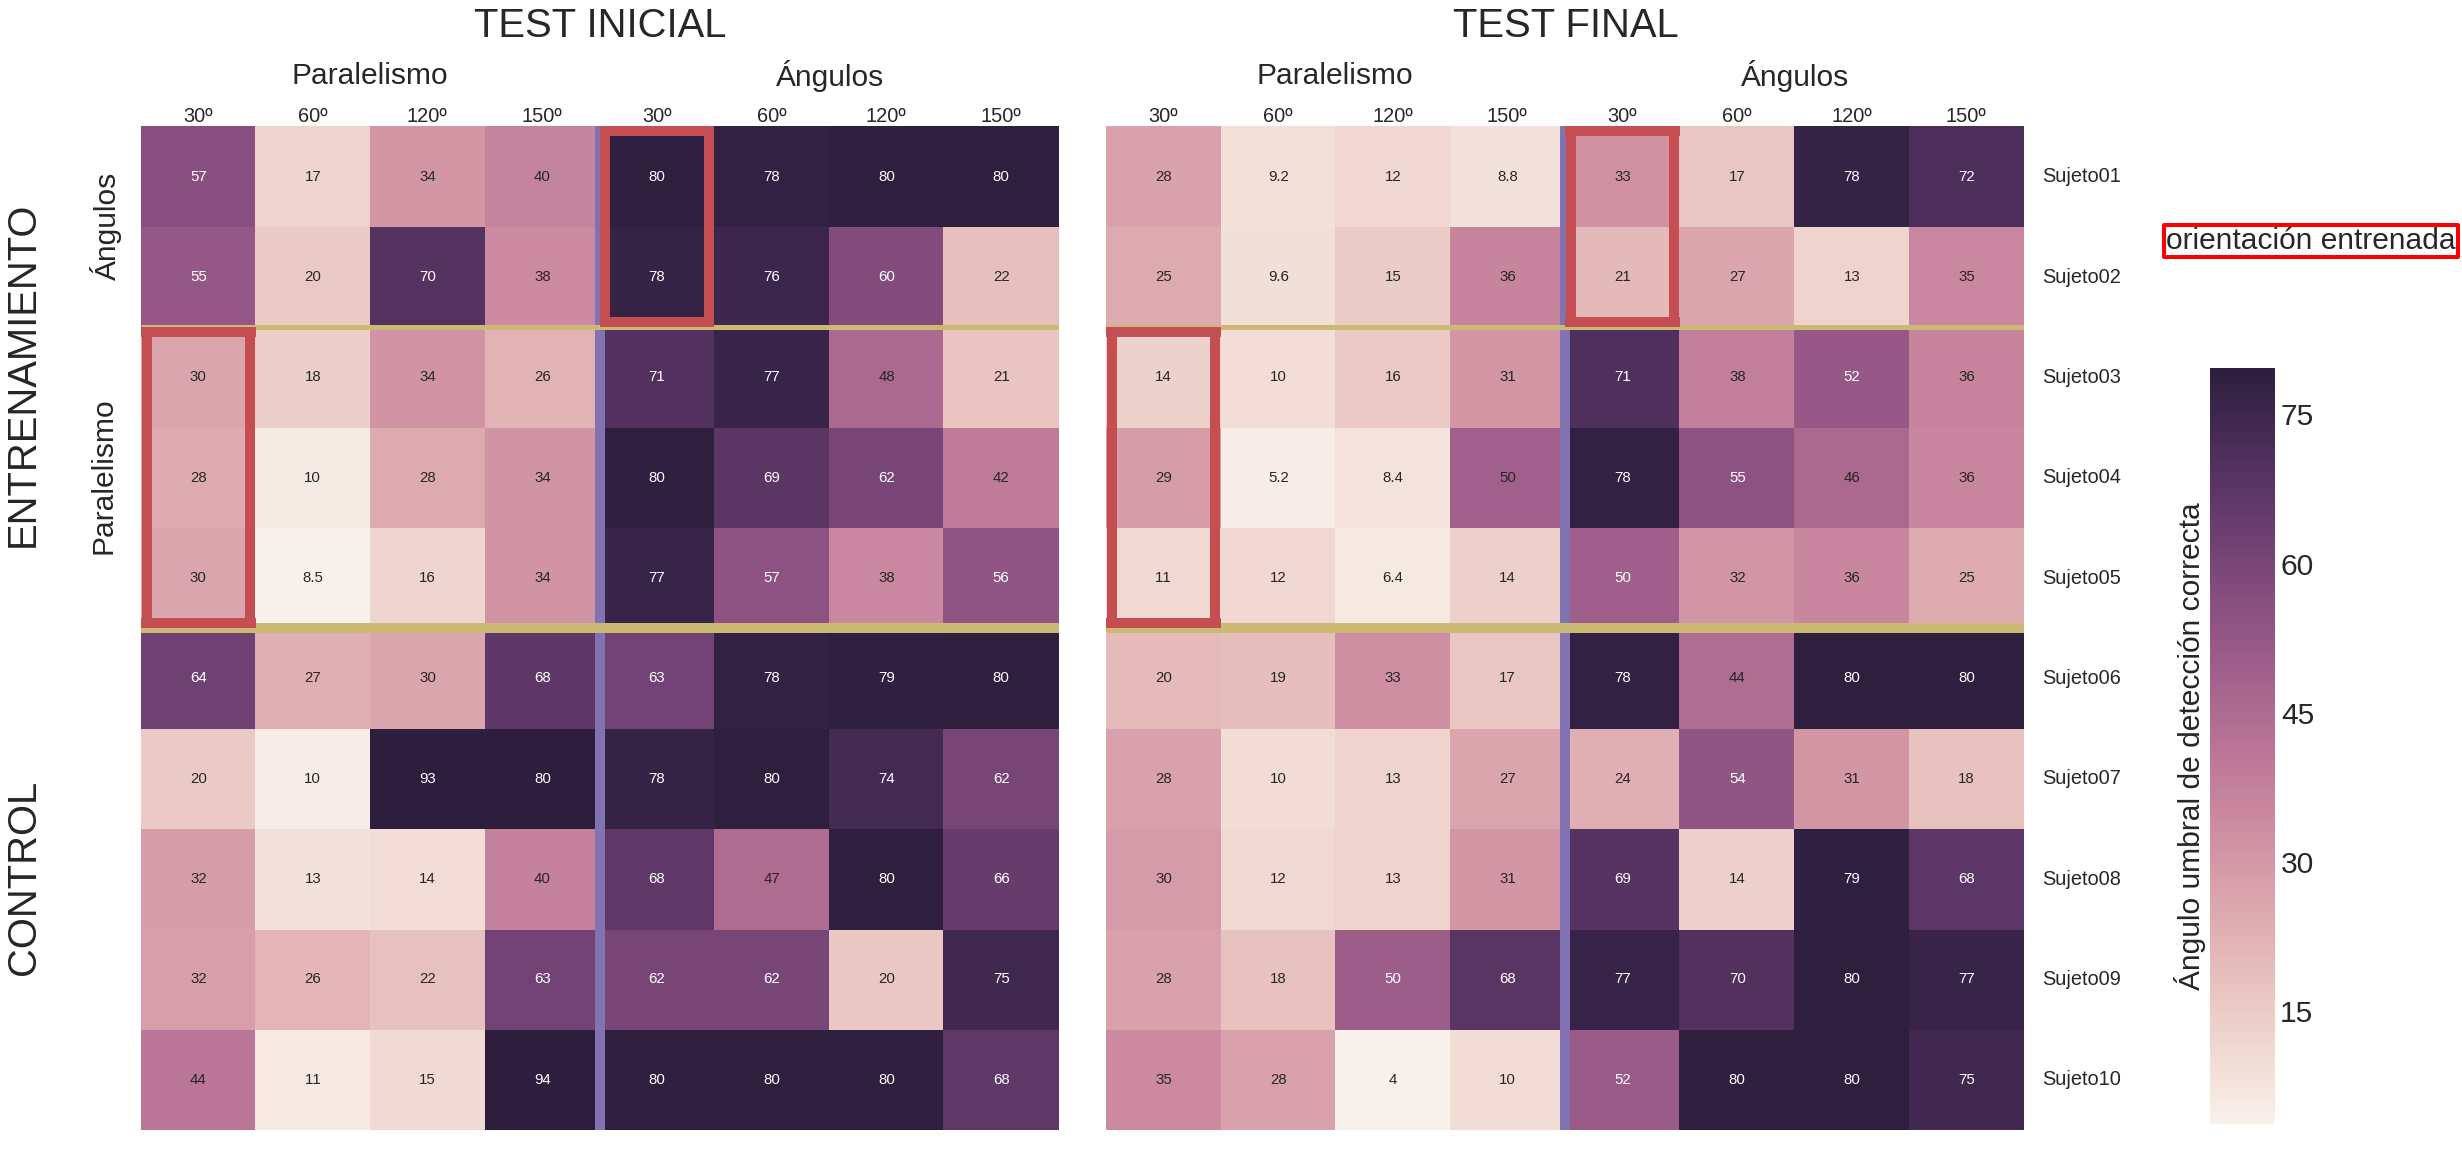
\includegraphics[width=\textwidth]{Imagenes/TransferenciaHeatmap.png}
        \caption{Mediciones de umbral obtenidas en la evaluación inicial y final del experimento de entrenamiento. Cada linea representa un sujeto y cada columna un experimento realizado. Se agrupa a los sujetos según que tipo de entrenamiento realizaron.}
        \label{fig:Exp2_Test}
    \end{figure}  
    
    
    \begin{figure}
        \center
        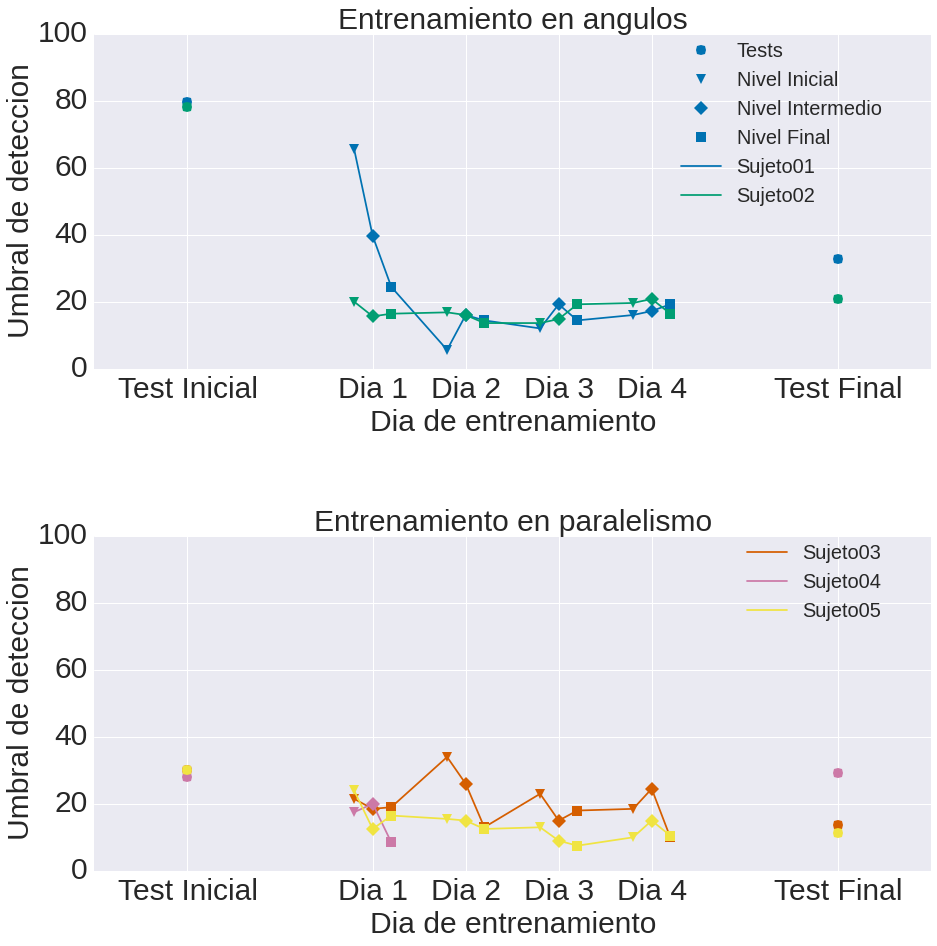
\includegraphics[width=\textwidth]{Imagenes/TransferenciaEntrenamientoNuevo.png}
        \caption{Mediciones obtenidas durante los entrenamientos realizados a los sujetos. Cada sujeto (excepto uno) realizó cuatro sesiones de entrenamiento en cada una de las cuales realizó tres niveles. El tiempo transcurrido entre sesión y sesión fue de unos pocos dias.}
        \label{fig:Exp2_Entrenamiento}
    \end{figure}  


    \subsubsection{Estudio del proceso de entrenamiento} \label{seccion:Exp2}
    
    Para analizar el proceso de entrenamiento nos propusimos estudiar cuatro indicadores, el primero fue si se observa un proceso global de mejora en los sujetos a lo largo del entrenamiento, el segundo si se observar una fluctuación dentro de cada sesión como proceso de entrenamiento diario, el tercero si el hecho de dar o no dar feedback afecta el umbral de percepción como un efecto agregado a la eventual mejora que el feedback proporcione en forma acumulada, y el cuarto, si las mediciones de las evaluaciones iniciales y finales se pueden enmarcar en el proceso de entrenamiento o si dan medidas diferentes a lo esperado como proyección del entrenamiento. 
    
    Para realizar todos estos estudios analizamos los datos realizando regresiones lineales con un modelo que agrupara la información con denominados 'efecto fijo' que permiten agrupar la información según corresponda a cada análisis. Para el primer caso por ejemplo, el ajuste debería ser de la forma:
    
    \begin{equation} \label{ec:RegresionEntrenamiento1}
        Y(i,t) = \beta \cdot t + cte_i
    \end{equation}
    
    donde t representa el numero de nivel realizado (considerando todos los niveles realizados por un mismo usuario como una serie) e i indica el sujeto analizado, o la variable en función de la cual se comparar.

    Para realizar este ajuste en forma de regresión lineal lo que debemos hacer es transformar los datos en la solución de una matriz donde una columna representa la repetición de la secuencia temporal (como denominamos a la variable t) y otras tantas columnas con indicadores binarios (ceros o unos) como criterios de agrupamiento de datos se quiera realizar. Ejemplificado este proceso para un caso de cuatro niveles de entrenamiento y tres sujetos donde se quiere analizar la progresion en el tiempo del umbral, quedaría un sistema de la forma de la ecuación \ref{ec:MatrixExpandida}.

    \begin{equation} \label{ec:MatrixExpandida}
    \bar {Y} = \bar{\delta} \cdot \bar{\bar{X}} \text{ con } \bar{\bar{X}} =
     \begin{pmatrix}
        %\beta & \alpha_1 & \alpha_2 & \alpha_3 & \gamma_{inicial} & \gamma_{final} \\
        0 & 1 & 0 & 0\\
        1 & 1 & 0 & 0\\
        2 & 1 & 0 & 0\\
        3 & 1 & 0 & 0\\
        0 & 0 & 1 & 0\\
        1 & 0 & 1 & 0\\
        2 & 0 & 1 & 0\\
        3 & 0 & 1 & 0\\
        0 & 0 & 0 & 1\\
        1 & 0 & 0 & 1\\
        2 & 0 & 0 & 1\\
        3 & 0 & 0 & 1\\
     \end{pmatrix} \text{ y $\bar{\delta}=(\beta,\alpha_1,\alpha_2,\alpha_3)$ el conjunto de parámetros a ajustar}
 \end{equation}
 
    Si en cambio se quisiera evaluar si el nivel intermedio de cada sesión difiere en forma significativa de la tendencia dada por los niveles iniciales y finales, para el caso simplificado donde dos sujetos realizaron dos sesiones de tres niveles, se debería ajusta el conjunto de parámetros dados por el sistema de la ecuación \ref{ec:Matrix2doDia}, donde se agrega una contante equivalente a ajustar la ordenada al origen (que en el caso anterior estaba incluida para cada sujeto en los $\alpha_i$), y se debe revisar si la variable $\alpha$ de este ajuste da significativamente distinta de cero. Mientras el conjunto de datos este correctamente balanceado respecto al numero de usuarios y demás variable que distingan el origen de las mediciones.

    \begin{equation} \label{ec:Matrix2doDia}
    \bar {Y} = \bar{\delta} \cdot \bar{\bar{X}} \text{ con } \bar{\bar{X}} =
     \begin{pmatrix}
        %\beta & \alpha_1 & \alpha_2 & \alpha_3 & \gamma_{inicial} & \gamma_{final} \\
        0 & 1 & 0\\
        1 & 1 & 1\\
        2 & 1 & 0\\
        3 & 1 & 0\\
        4 & 1 & 1\\
        5 & 1 & 0\\
        0 & 1 & 0\\
        1 & 1 & 1\\
        2 & 1 & 0\\
        3 & 1 & 0\\
        4 & 1 & 1\\
        5 & 1 & 0\\
     \end{pmatrix} \text{ y $\bar{\delta}=(\beta,cte,\alpha)$ el conjunto de parámetros a ajustar}
    \end{equation}

    Con el criterio mencionado lo primero que hicimos fue analizar la tendencia global del umbral medido a lo largo del entrenamiento. Para este análisis descartamos al sujeto 4 que solo realizo el primer día de entrenamiento. 
    
    En la tabla \ref{tabla:entrenamientoGlobalParalelismo} se puede observar el resultado que arroja el algoritmo utilizado (\url{http://statsmodels.sourceforge.net/devel/generated/statsmodels.regression.linear_model.OLS.html}). Se puede observar que se encontró una pendiente (que aunque leve es significativa). Si para este análisis se quita los efectos fijos (y se agrega una ordenada al origen comun a todos los datos) el valor obtenido de la pendiente no varia, pero aumenta su pValor que pasa a ser (0.054) que si bien resulta en una pendiente no significativa esta muy proxima a serlo. Esta fluctuación tiene que ver con como el algoritmo estima los errores según tenga más variable de ajuste. 
    
    Realizando el mismo análisis para los datos del entrenamiento en ángulos nos encontramos con el problema de que hay una sesión (la primera del sujeto1) que muestra un comportamiento claramente diferente al resto. Si realizamos el ajuste como en el caso anterior observamos (ver tabla \ref{tabla:betas}) una pendiente mucho mayor, pero que el resultado no es significativo. Frente a esto decidimos analizar los datos excluyendo o bien al sujeto 1 o bien el día 1 de entrenamiento, para ver si se encontraba alguna tendencia significativa. En el primer caso resulto que no, y en el segundo que si, pero en ambos casos la pendiente es positiva (es decir que los sujetos empeorarían su umbral). En cualquier caso, todos los valores de pendiente obtenidos son del orden de la unidad o menores (entre nivel y nivel), lo cual, comparado con los valores medios de umbral, claramente no indica una progresión relevante en la escala temporal medida, mas allá del bajo numero de sujetos que impiden obtener una conclusión extrapolable a una población general.  
    
    Por otro lado quisimos estudiar si hay un efecto diario de entrenamiento. En este caso se observa un efecto significativo de mejora entre el primer y el ultimo resultado de cada sesión de aproximadamente 7º para las pruebas de paralelismo, mientras que para el entrenamiento de ángulos no se observa ningún resultado significativo, se incluya o no la sesión en que el sujeto 1 muestra un comportamiento marcadamente diferente.
    
    En cuanto al estudio de si la presencia de feedback implica una mejora en el resultado de umbral medido por su mera presencia no se pudo observar ningún efecto significativo. Por último lo que hicimos fue ajustar los resultados del test inicial y final como si fueran el primer y ultimo entrenamiento, para evaluar si hay una salto cualitativo entre los resultados ya sea porque el contexto es diferente o porque entre las evaluaciones y el entrenamiento se da algún cambio (por ejemplo la devolución de feedback) cualitativo. En este caso si se dio un efecto significativo y muy marcado para el salto inicial y mucho menos marcado (en paralelismo dio no significativo) para el salto final. Una posible explicación a este efecto podría ser que la presencia de feedback que el sujeto recibe por primera vez en la primer sesión del entrenamiento afecte en forma cualitativa la percepción presente y futura del sujeto. Otra explicación posible puede deberse a que durante la evaluación inicial el sujeto realice un proceso de entrenamiento por más que cada nivel este orientado en una dirección diferente. En el diseño experimental se resolvió que los sujetos entrenen en la orientación correspondiente al primer nivel de evaluación, sin embargo los estudios que realizamos al analizar las evaluaciones iniciales y finales no parecen ser compatibles con esta hipótesis. 

    \begin {table}

    \begin{center}

    \caption{Ejemplo de resultados obtenidos: caso de la regresión OLS para el conjunto de todas las mediciones durante el entrenamiento de los sujetos 3 y 5 que entrenaron paralelismo donde se busca encontrar un efecto de mejora global.}
    \label{tabla:entrenamientoGlobalParalelismo}

    \vspace{0.3in}
    \begin{tabular}{lclc}
    \toprule
    \textbf{Dep. Variable:}    &        y         & \textbf{  R-squared:         } &     0.448   \\
    \textbf{Model:}            &       OLS        & \textbf{  Adj. R-squared:    } &     0.395   \\
    \textbf{Method:}           &  Least Squares   & \textbf{  F-statistic:       } &     8.506   \\
    \textbf{Date:}             & Mon, 28 Nov 2016 & \textbf{  Prob (F-statistic):} &  0.00197    \\
    \textbf{Time:}             &     11:22:28     & \textbf{  Log-Likelihood:    } &   -70.703   \\
    \textbf{No. Observations:} &          24      & \textbf{  AIC:               } &     147.4   \\
    \textbf{Df Residuals:}     &          21      & \textbf{  BIC:               } &     150.9   \\
    \textbf{Df Model:}         &           2      & \textbf{                     } &             \\
    \bottomrule
    \end{tabular}

    \begin{tabular}{lccccc}
                & \textbf{coef} & \textbf{std err} & \textbf{t} & \textbf{P$>|t|$} & \textbf{[95.0\% Conf. Int.]}  \\
    \midrule
    $\beta$ &      -0.7133  &        0.291     &    -2.451  &         0.023        &        -1.319    -0.108       \\
    $\alpha_{3}$ &      24.0064  &        2.141     &    11.215  &         0.000        &        19.555    28.458       \\
    $\alpha_{5}$&      17.3397  &        2.141     &     8.101  &         0.000        &        12.888    21.791       \\
    \bottomrule
    \end{tabular}
    
    \begin{tabular}{lclc}
    \textbf{Omnibus:}       &  3.425 & \textbf{  Durbin-Watson:     } &    2.461  \\
    \textbf{Prob(Omnibus):} &  0.180 & \textbf{  Jarque-Bera (JB):  } &    2.201  \\
    \textbf{Skew:}          &  0.736 & \textbf{  Prob(JB):          } &    0.333  \\
    \textbf{Kurtosis:}      &  3.191 & \textbf{  Cond. No.          } &     17.4  \\
    \bottomrule
    \end{tabular}
    
    \end{center}
    
    \end{table}


    % Vamos con los resultados obtenidos
    
    \begin{table}

    \begin{center}
    
    \caption{Ajustes realizados sobre las mediciones del entrenamiento y sus respectivos resultados}
    \label{tabla:betas}
    \vspace{0.3in}
    
    \begin{tabular}{lcc}
                Estudio realizado & Valor obtenido & P$>|$t$|$ \\
    \midrule
    \midrule
    
    Pendiente global paralelismo  &  -0.7133  &  \textbf{0.023} \\
    Pendiente global ángulos      &  -1.1916  &  0.077 \\
    Pendiente global ángulos excluyendo sujeto 1 &  0.0671  & 0.768 \\
    Pendiente global ángulos excluyendo dia 1    &  0.7833  & \textbf{0.009} \\
    Pendiente diaria paralelismo  &  -3.4167  &  \textbf{0.016} \\
    Pendiente diario ángulos      &  -1.9500  &  0.453 \\
    Pendiente diario ángulos excluyendo dia 1 sujeto 1 &  0.7143   &  0.402 \\
    Corrimiento de las mediciones sin feedback (ángulos)  &  1.5714  &  0.288 \\
    Corrimiento de las mediciones sin feedback (paralelismo)  &  1.0278  &  0.662 \\
    Salto inicial paralelismo     &  9.3047  &  \textbf{0.022} \\
    Salto inicial ángulos          &  65.3283  &  \textbf{0.000} \\
    Salto final paralelismo       &  5.5221  &  0.202 \\
    Salto final ángulos          &  8.7894  &  \textbf{0.011} \\
    
    \bottomrule
    \end{tabular}
    
    \end{center}
    
    \end{table}


\subsubsection{Estudio comparativo de la evaluación inicial y final.}

    A la hora de evaluar los resultados obtenidos en la figura \ref{fig:Exp2_Test} donde se observan los datos correspondientes a la evaluación inicial y final surgen dos posibles criterios de análisis. Por un lado las comparaciones entre experimentos (combinaciones de categoría y orientación) y por otro lado las comparaciones entre sujetos. En todos los casos el mayor limitante a la hora de obtener resultados validos fue el bajo numero de sujetos. 
    
    Para la comparación entre experimentos utilizamos los datos correspondientes a la evaluación inicial, ya que en este caso tenemos diez sujetos que realizaron todos los mismo experimento en igualdad de condiciones, por lo tanto tenemos un numero de sujetos que aunque reducido permite hacer ciertos análisis estadísticos. Al diseñar el experimento esperábamos observa cierto efecto del entrenamiento durante la ejecución de las evaluaciones, lo que no sabíamos era cuan relevante resultaría en relación al efecto de entrenamiento en una orientación especifica que era lo que queríamos poder diferenciar. Teniendo en cuanta los resultados del análisis del entrenamiento, donde se observa un salto cualitativo inicial y una saturación en el efecto del entrenamiento (al menos en la escala de duración estudiada), podría suceder que el entrenamiento durante la evaluación sea marcada mostrando una progresion en función del numero de experimentos realizados. 
    
    Para evaluar esta hipótesis comparamos los desempeños agrupando por experimento realizados. Los datos y los resultados pueden observarse en las figuras \ref{fig:Exp2_HistoInicial} y \ref{fig:Exp2_SignificanciaInicial} donde no se observa el efecto esperado. En el caso de paralelismo al realizar un Anova el único grupo de mediciones diferenciado resulto ser el de la orientación 60º (carecemos de una explicación que justifique este hecho mas allá de atribuirlo a una fluctuación estadística), en el caso de los ángulos al realizar un Anova no se puede distinguir ninguna de las muestras de las demás. 
    
    Sin embargo, mirando los datos, en el caso de los ángulos parecería haber un tendencia, pero hay que tener cuidado de atribuirla a un efecto de entrenamiento progresivo ya que la mayoría de las mediciones consideradas están en la zona de saturación de la escala, indicando que los sujetos no son capaces de distinguir entre categorías en absoluto. Por lo tanto el corrimiento del umbral promedio (que se correlaciona con un aumento de la desviación) puede deberse mas a un efecto de que algunos sujetos empiezan a distinguir entre los estímulos (y por lo tanto salen de la zona de saturación) que a una mejora cuantitativa. Pero los valores medidos, incluso para los sujetos con umbral bajo siguen estando lejos del nivel que reportan los sujetos entrenados tras la primer sesión. 
    
    \begin{figure}
        \center
        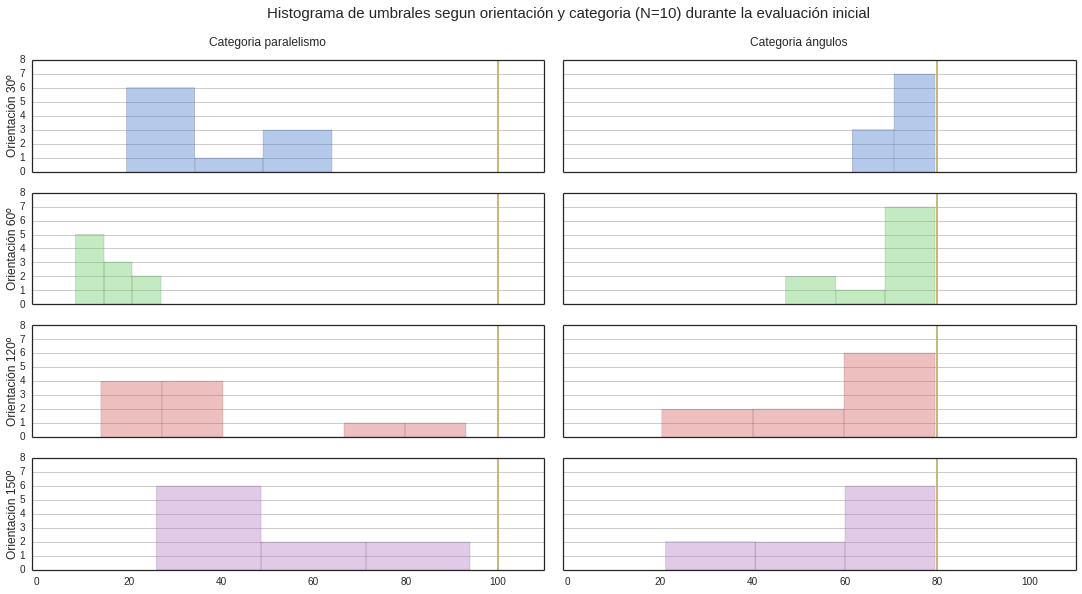
\includegraphics[width=\textwidth]{Imagenes/TransferenciaInicialHisto.png}
        \caption{Histogramas donde se puede observar la distribución de umbrales de detección en función de la orientación y la categoría medida. Todos los sujetos realizaron los experimentos en el mismo orden en sentido antihorario de orientaciones, haciendo primero todas las pruebas de paralelismo y luego las de ángulos. Se observa que en el caso de los ángulos la mayor parte de las mediciones satura en el nivel de máxima señal permitida (linea vertical amarilla) mientras que en el caso de paralelismo esto no sucede.}
        \label{fig:Exp2_HistoInicial}
    \end{figure}  

    \begin{figure}
        \center
        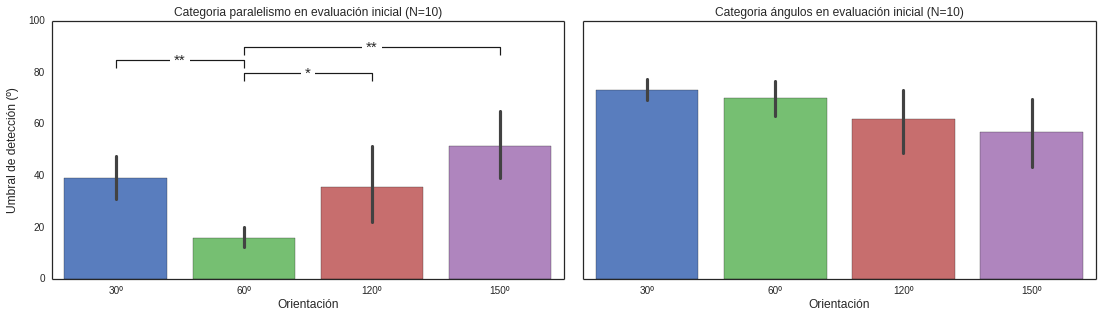
\includegraphics[width=\textwidth]{Imagenes/TransferenciaInicialMedias.png}
        \caption{Comparación estadistica de las medidas observadas en la figura \ref{fig:Exp2_HistoInicial}. Luego de realizar un Anova comparando todas las mediciones dentro de cada categoría, solo se detectó una diferencia significativa debido al grupo de mediciones orientadas en 60 en el caso de paralelismo. Para esta orientación se realizó un análisis Ttest (considerando correlación) y se observan diferencias significativas con todos los demás grupos. La razón de esta diferencia la desconocemos.}
        \label{fig:Exp2_SignificanciaInicial}
    \end{figure}  
    
    De este análisis también esperábamos observar si había algún tipo de parámetro relacionado a la orientación que influyera en la dificultad de reconocer los estímulos. Al parecer (al menos con la reducida muestra de datos que tenemos) no hay patrón de dificultad relacionado con la orientación pues incluso el conjunto de mediciones realizadas en paralelismo a 60º  no se explica en base a su orientación considerando las simetrías en común que tiene con los demás estímulos.
    
    Por último queda comparar entre los sujetos y su desempeño según cual haya sido el entrenamiento realizado. En este caso debido al bajo numero de sujetos no tiene sentido hacer un análisis estadístico pero en las figuras \ref{fig:TransferenciaParalelismo} y \ref{fig:TransferenciaAngulos} se puede observar la información antes de promediar entre los sujetos que entrenaron en la misma categoria y en las figuras \ref{fig:TransferenciaParalelismoBarras} y \ref{fig:TransferenciaAngulosBarras} se puede observar la misma información agrupada según entrenamiento. 
    
    Si bien estas figuras solo sirven para visualizar la información y asumir tendencias (pues la mayoría de las comparaciones no pasa un test estadístico que por otro lado no tiene sentido realizar), se puede ver que en todos los casos hay una mejora en el umbral de detección en la medición final respecto a la inicial, y que en algunos casos es muy marcado (en particular para los dos sujetos que entrenaron ángulos la mejora parece ser superior a los demás en todas las categorías). Tambien se destaca las comparaciones que en ambos casos, los sujetos que entrenaron, mejoran mas en la orientación entrenada que en las no entrenadas, si bien no parece ser que mejoren mas que los sujetos control. Pero todas estas observaciones requieren de más mediciones para ser consideradas como válidas.
    
    \begin{figure}
        \center
        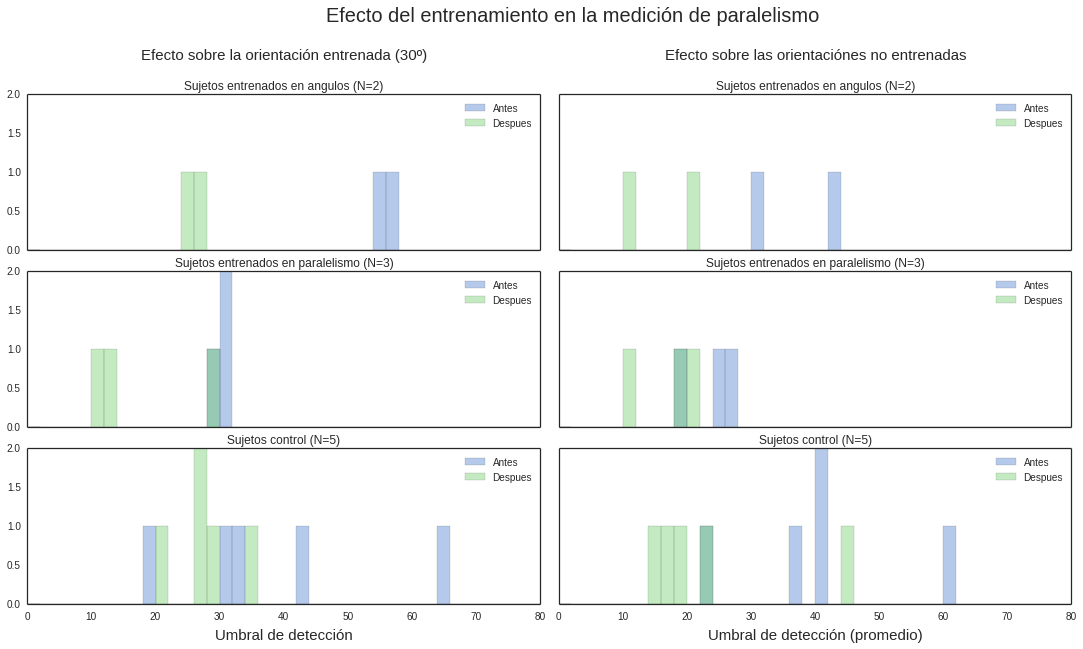
\includegraphics[width=\textwidth]{Imagenes/TransferenciaParalelismo.png}
        \caption{Detalle de los resultados para el entrenamiento de paralelismo donde se puede comparar las mediciones obtenidas tanto en la orientación entrenada como en las que no para los sujetos que realizaron diferentes procesos de entrenamiento. En la figura \ref{fig:TransferenciaParalelismoBarras} se puede ver estos datos promediados.}
        \label{fig:TransferenciaParalelismo}
    \end{figure}  

    \begin{figure}
        \center
        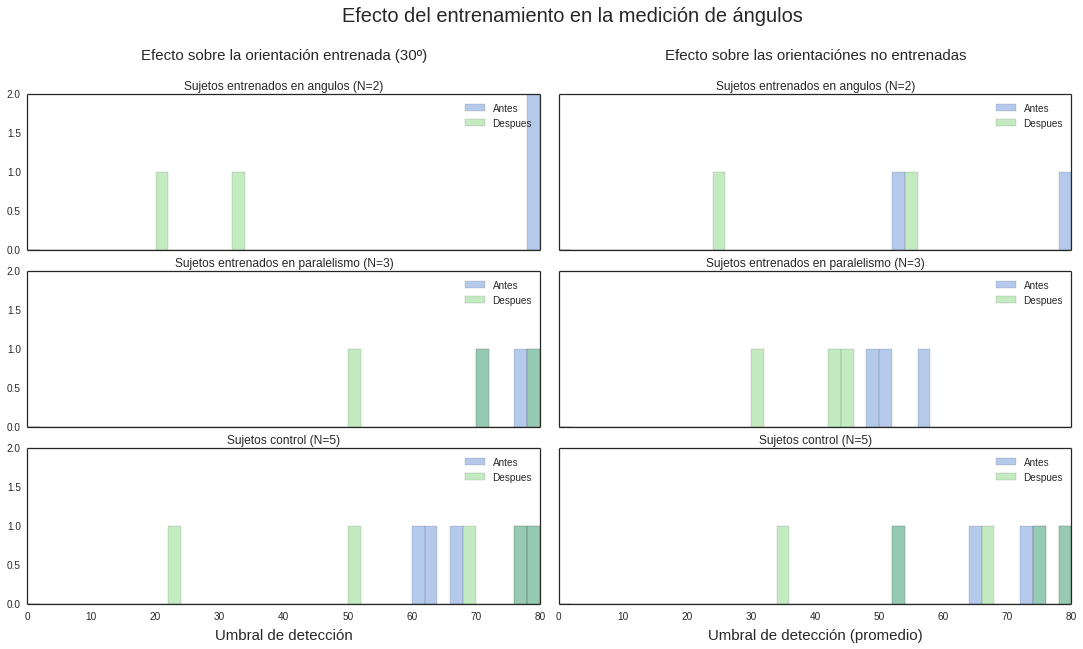
\includegraphics[width=\textwidth]{Imagenes/TransferenciaAngulos.png}
        \caption{Detalle de los resultados para el entrenamiento de ángulos donde se puede comparar las mediciones obtenidas tanto en la orientación entrenada como en las que no para los sujetos que realizaron diferentes procesos de entrenamiento. En la figura \ref{fig:TransferenciaAngulosBarras} se puede ver estos datos promediados.}
        \label{fig:TransferenciaAngulos}
    \end{figure}  
    
        \begin{figure}
        \center
        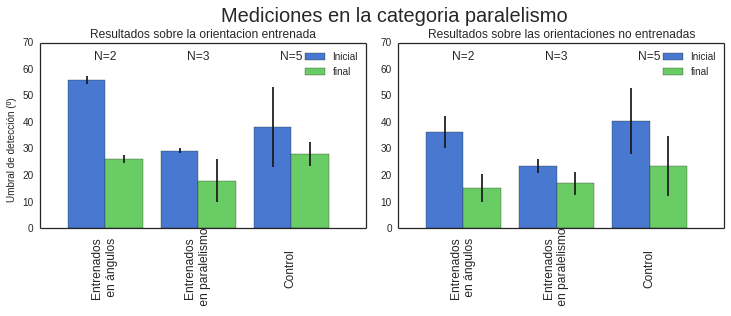
\includegraphics[width=\textwidth]{Imagenes/TransferenciaParalelismoBarras.png}
        \caption{Comparación de medidas de umbral para las mediciones de paralelismo, promediando entre sujetos según entrenamiento realizado comparando el umbral entre la evaluación inicial y la evaluación final.}
        \label{fig:TransferenciaParalelismoBarras}
    \end{figure}  

    \begin{figure}
        \center
        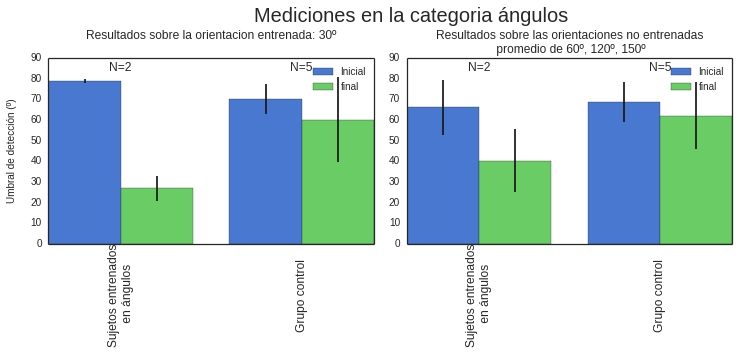
\includegraphics[width=\textwidth]{Imagenes/TransferenciaAngulosBarras.png}
        \caption{Comparación de medidas de umbral para las mediciones de ángulos, promediando entre sujetos según entrenamiento realizado comparando el umbral entre la evaluación inicial y la evaluación final.}
        \label{fig:TransferenciaAngulosBarras}
    \end{figure}  
    
    
    

\clearpage


\begin{thebibliography}{9}

\bibitem{NroCiegos}
  WHO (2011) Fact Sheet Nu282
\bibitem{Implantes1}
Dowling J (2008) Current and future prospects for optoelectronic retinal prostheses. Eye 23: 1999–2005.
\bibitem{Implantes2}
Weiland JD, Cho AK, Humayun MS (2011) Retinal prostheses: current clinical results and future needs. Ophthalmology 118: 2227–2237.
\bibitem{Implantes3}
E Striem-Amit, A Bubic, A Amedi - 2012: Neurophysiological Mechanisms Underlying Plastic Changes and Rehabilitation following Sensory Loss in Blindness and Deafness
\bibitem{Implantes4}
Zrenner E, Bartz-Schmidt KU, Benav H, Besch D, Bruckmann A, et al. (2010) Subretinal electronic chips allow blind patients to read letters and combine them to words. Proceedings of the Royal Society B: Biological Sciences 278: 1489–1497.
\bibitem{Tactil1}
Bach-Y-Rita P, Collins C.C, Saunders F.A, White B, Scadden L. Vision substitution by tactile image projection. Nature. 1969;221:963–964. 
\bibitem{Tactil2}
Bach-Y-Rita P, Kaczmarek K.A, Tyler M.E, Garcia-Lara J. Form perception with a 49-point electrotactile stimulus array on the tongue: A technical note. J Rehabil Res Dev. 1998;35:427–430.
\bibitem{Tactil3}
Sampaio E, Maris S, Bach-Y-Rita P. Brain plasticity: ‘Visual’ acuity of blind persons via the tongue. Brain Res. 2001;908:204–207. 
\bibitem{Tactil4}
Chebat D.R, Rainville C, Kupers R, Ptito M. Tactile-‘visual’ acuity of the tongue in early blind individuals. Neuroreport. 2007;18:1901–1904
\bibitem{Voice1}
Meijer P.B. An experimental system for auditory image representations. IEEE Trans Biomed Eng. 1992;39:112–121.
\bibitem{VoiceVariante1}
Capelle C, Trullemans C, Arno P, Veraart C. A real-time experimental prototype for enhancement of vision rehabilitation using auditory substitution. IEEE Trans Biomed Eng. 1998;45:1279–1293. 
\bibitem{VoiceVariantes2}
Cronly-Dillon J, Persaud K, Gregory R.P. The perception of visual images encoded in musical form: A study in cross-modality information transfer. Proc Biol Sci. 1999;266:2427–2433. 
\bibitem{VoiceVariantes3}
Cronly-Dillon J, Persaud K.C, Blore R. Blind subjects construct conscious mental images of visual scenes encoded in musical form. Proc Biol Sci. 2000;267:2231–2238.
\bibitem{VoiceVariantes4}
Abboud, Sami, et al. "EyeMusic: Introducing a “visual” colorful experience for the blind using auditory sensory substitution." Restorative neurology and neuroscience 32.2 (2014): 247-257.
\bibitem{VoiceSubyacente1}
Poirier, Colline, Anne G. De Volder, and Christian Scheiber. "What neuroimaging tells us about sensory substitution." Neuroscience and Biobehavioral Reviews 31.7 (2007): 1064-1070.
\bibitem{VoiceSubyacente2}
Arno P, Capelle C, Wanet-Defalque M.C, Catalan-Ahumada M, Veraart C. Auditory coding of visual patterns for the blind. Perception. 1999;28:1013–1029. [PubMed]
\bibitem{VoiceSubyacente3}
Arno P, De Volder A.G, Vanlierde A. et al. Occipital activation by pattern recognition in the early blind using auditory substitution for vision. Neuroimage. 2001;13:632–645.
\bibitem{VoiceSubyacente4}
Auvray M, Hanneton S, O’Regan J.K. Learning to perceive with a visuo-auditory substitution system: Localisation and object recognition with ‘The vOICe’ Perception. 2007;36:416–430.
\bibitem{VoiceEntrenamiento1}
Striem-Amit, Ella, Miriam Guendelman, and Amir Amedi. "‘Visual’acuity of the congenitally blind using visual-to-auditory sensory substitution." PloS one 7.3 (2012): e33136.
\bibitem{VoiceEntrenamiento2}
Striem-Amit, Ella, et al. "Reading with sounds: sensory substitution selectively activates the visual word form area in the blind." Neuron 76.3 (2012): 640-652.
\bibitem{VoiceEntrenamiento3}
Arno, Patricia, et al. "Auditory substitution of vision: pattern recognition by the blind." Applied Cognitive Psychology 15.5 (2001): 509-519.
\bibitem{staircase}
Levitt, H. C. C. H. "Transformed up down methods in psychoacoustics." The Journal of the Acoustical society of America 49.2B (1971): 467-477.
\end{thebibliography}


\clearpage

\section{Anexos}
\subsection{Descripción de las clases que conforman a la plataforma con la que se realizó y construyo los experimentos} \label{anexo:Clases}

    \begin{itemize}
        \item \textit{\textbf{com.turin.tur.main.screens}}
        \begin{itemize}
            \item \textbf{AbstractGameScreen:} Es una clase genérica (copiada de un ejemplo en internet) que sirve para implementar pantallas en videojuegos. Al ser una clase abstracta no implementa ningún método por si misma, sino que fuerza a todas las pantallas a que tengan definidos los métodos correspondientes. 
            \item \textbf{InstructionScreen:} Diseño de una pantalla con instrucciones que se escribió pensando en una ejecución de los experimentos fuera de laboratorio donde la explicación de la tarea a realizar tenía que darla la misma aplicación.
            \item \textbf{MenuScreen:} Pantalla principal de la aplicación (ver figura \ref{fig:Pantallas1}). A partir de la información de los niveles disponibles así como de la información de lo ya realizado por el sujeto habilita al usuario a realizar los niveles que correspondan. En la ultima versión del experimento, además se implemento un sistema por el cual la aplicación reconocía en que sesion del entrenamiento se encontraba el sujeto y por lo tanto ajustaba los niveles disponibles según correspondiera a los tests iniciales o finales o al proceso de entrenamiento. 
            \item \textbf{LevelScreen:} Pantalla en la que se desarrolla la secuencia de trials. En si misma no hace mucho excepto cargar el LevelController y el LevelRender encargados de manipular el contenido del nivel. 
            \item \textbf{ResultsScreen:} Pantalla que fue diseñada como devolución al usuario de su desempeño en el nivel realizado (ver figura \ref{fig:Pantallas1}). Esta pantalla tenia sentido en tanto pensabamos un diseño de la aplicación compatible con experimentos masivos y en contextos externos al laboratorio en donde había que darle una devolución al usuario y además comprobar si había superado los requerimientos básicos del nivel realizado. Salvo en una etapa inicial del proyecto esta pantalla fue discontinuada. 
        \end{itemize}
        
        \item \textit{\textbf{com.turin.tur.obsoleto.Stadistics:}} En este paquete quedaron guardadas las herramientas necesarias para realizar los cálculos estadísticos realizados al finalizar los niveles en la versión preliminar en la que se mostraba la pantalla de resultados. La idea era que el programa pudiera calcular en función del desempeño del usuario si estaba preparado o no para pasar de nivel. Para eso debía comparar los resultados contra distribuciones estadísticas y revisar que el buen desempeño no fuera producto del azar. Como LibGDX esta pensado para desarrollar videojuegos este tipo de cálculos no vienen incluidos entre las librerías que soporta (y al ser necesaria la ejecución en tiempo real eventualmente en celulares o internet no podíamos usar opciones disponibles solo para PC externas al paquete LibGDX), por lo que debimos resolver y escribir funciones estadísticas típicas del calculo de distribuciones (pero en nuestro caso con numero variable de opciones por trial). Todo esto quedo obsoleto al decidir que los experimentos se realizarían en un entorno tradicional de laboratorio. 
        
        \item \textit{\textbf{com.turin.tur.main.diseno:} Este paquete incluye todas las clases accesorias que hacen a la manipulación del contenido de la aplicación en forma de objetos y cuyo contenido es cargado por el diseño general de los niveles y el LevelController}.
        \begin{itemize}
            \item \textbf{ExperimentalObject:} Clase que guarda la información del objeto experimental (estímulo y toda su información conceptual asociada). Así como métodos para cargar la información desde los archivos "meta", "mp3" o "atlas" almacenados en disco. 
            \item \textbf{Boxes:} Clase que se encarga de la manipulación de los ExperimentalObject según el contexto. Cada caja carga un objeto experimental, pero según se trate de un trial de tutorial, de entrenamiento o de test se comporta diferente. En los trials de tutorial, al seleccionar una caja (TrainingBox) se activa la reproducción del sonido correspondiente, en los trials de test hay dos tipos de cajas diferentes, la del estimulo (StimuliBox) y la de las respuestas (OptionBox). La del estimulo no es seleccionable y reproduce en forma automatica el sonido correspondiente a su contenido (y muestra una imagen predeterminada de signo de interrogación (ver figura \ref{fig:Pantallas2}), en cambio las cajas de respuesta muestran la imagen correspondiente a su contenido (que puede ser una categoría abstracta o una figura y al ser seleccionadas solo activan el paso de trial (previa respuesta de feedback si correspondiera).  
            \item \textbf{RunningSound:} Clase que se carga junto al nivel y que se encarga de manipular la reproducción de los sonidos provenientes de los estímulos. Se creo una clase aparte para evitar reproducciones simultaneas y para poder pausar, iniciar y detener las reproducciones de sonido de manera unificada. 
            \item \textbf{TouchInfo:} Clase que crea con cada toque en pantalla. Almacena la información de las coordenadas (tanto en pantalla como en el espacio geometricos de representacion del la aplicacion), y del objeto que fue tocado, junto a la información contextual en que sucedio el toque. Esta clase se creo en forma independiente para poder realizar un seguimiento exaustivo de la actividad que realiza el sujeto y poder enviar al servidor paquetes de datos con toda la información de lo sucedido de forma de poder recrear la actividad del sujeto por completo. Sin embargo el volumen de información generado resultó desproporcionado y finalmente se envio un registro mucho menor de la actividad manipulada a traves de la clase Trial.
            \item \textbf{Session:} Es la clase encargada de manipular toda la información relacionada a la información global de la ejecusión del programa. Incluye la información del usuario, lo métodos para crear un usuario nuevo, el registro de niveles realizados, fases (días de entrenamiento) experimentales, e información de versiones del código y de los recursos manipulados. 
            \item \textbf{MedidosDeConfianza:} Implementa la interfaz gráficas, el registro y los métodos necesarios para incluir en los trials un reporte de confianza en la respuesta dada. En un momento consideramos incluir esta medición para observar los efectos del entrenamiento en la confianza reportada, pero luego a partir de problemas de incompatibilidad entre los diseños experimentales excluimos del diseño general esta implementación. 
            \item \textbf{Trial:} Clase que engloba toda la información correspondiente a un trial. Tiene métodos para poder cargar desde los archivos de configuración el diseño correspondiente a cada trial (listado de estímulos, tipo de trial, disposición en pantalla) y para crear las correspondientes cajas (Boxes) en pantalla. Durante el proceso de creación de estímulos y niveles se instancian todos los posibles trials a realizar y vuelcan a disco de manera que en tiempo de ejecución puedan ser cargados por la lógica del diseño experimental incluida en los niveles.
            \item \textbf{LevelOLD:} Estructura obsoleta de un estadio inicial del desarrollo, cuando el diseño de los niveles era mas sencillo y no ameritaba un empaquetado aparte. 
            
        \end{itemize}
        
         \item \textit{\textbf{com.turin.tur.main.logic:} Este paquete contiene dos clases estandar pensadas para el loop principal de un videojuego. Una se encarga de manipular los eventos y otra de actualizar los gráficos.}.
         \begin{itemize}
             \item \textbf{LevelController:} Esta clase intercepta todos los comandos (click, toque en pantalla o presiones de teclado) que realiza el usuario y desencadena eventos en consecuencia. Puede alternar el estado de la aplicación entre diferentes estados (esperando respuesta, pantalla en blanco entre trial y trial, etc) y según el estado en que se encuentra el programa responder a diferentes estímulos. En cada iteración detecta toque en pantalla y genera los TouchInfo correspondientes que son enviados a la clase Trial si se toca algún Box adecuado. Tambien cheque constantemente el estado del trial y del RunningSound para activar el cambio de trial o la finalización del nivel cuando corresponda. Esta clase es la que interactúa con los métodos principales de los Levels para preguntarle que corresponde hacer en casa ocasión. 
             \item \textbf{LevelRender:} En cada iteración del LevelControler se desencadena la actualización de los gráficos en pantalla a través de esta clase. La clase además de graficar los elementos principales del trial le envía un evento a los Boxes y al RunningSound para que actualicen su estado (mover el indicador de reproducción en el Box que suena, indicar si debe mostrarse o no feedback, o regular el loop automático de los sonidos de estímulo)
         \end{itemize}
        
        \item \textit{\textbf{com.tur.tur.main.levelsDesign:} Este paquete incluye toda la estructura, configuración y métodos para manipular los niveles, tanto en tiempo de ejecución, como durante la creación de los estímulos y niveles.}
        \begin{itemize}
            \item \textbf{Level:} Clase abstracta que es implementada por todos los niveles a modo de interfaz para asegurar que dispongan de los métodos necesarios para el funcionamiento del programa. También incluye todas las subclases y métodos comunes que permiten generar estructuras conceptuales en forma automática en el Builder. 
            \item \textbf{LevelEjemplos:} Nivel que sirve para realizar el tutorial inicial. Este nivel no mide nada, simplemente es una secuencia de trials fija en los que se muestran estímulos que pueden ser reproducidos para escuchar su correspondiente sonido y comprender la lógica del vOICe. Esta clase incluye su propio constructor que crea los archivos y estímulos correspondientes al nivel utilizando las herramiendas del empaqueado Builder. 
            \item \textbf{LevelUmbralStatic:} Esta clase es la responsable de la creación de toda la estructura de datos necesaria para hacer experimentos del tipo detección de umbral (como los que terminamos haciendo). La logica con que se generan los niveles y recursos se detalla más adelante
            \item \textbf{LevelUmbral:} Esta clase maneja la dinámica interna de todos los niveles de tipo umbral en tiempo de ejecusión. Para eso cuenta la información de todos los estímulos disponibles para mostrar en dicho nivel, los trials correspondientes a cada estimulo, y la lógica con que debe indicar al LevelController los estímulos a mostrar (que se detalla en la sección \ref{seccion:staircase}). También tiene implementados los métodos que permiten que el LevelController le pase los eventos frente a los cuales actuar. Esta clase es la que observa si el Box tocado por el usuario se corresponde con la respuesta adecuada, y la que lleva el registro del desempeño del sujeto que es enviado a Internet al finalizar cada nivel. 
        \end{itemize}
        
        \item \textit{\textbf{com.turin.tur.main.util.builder:} Este paquete incluye todos los mecanismo y herramientas necesarias para construir la lista de estímulos y archivos que cada nivel requiere. Que construir esta definido en el paquete Level. La lógica detallada con que se contruyen los niveles se detalla en la sección \ref{seccion:builder}}
        \begin{itemize}
            \item \textbf{PcBuild:} Esta clase se inicializa solo si la aplicación esta ejecutandose en una PC y si esta activada el modo correspondientes en la configuración general del programa. Es el punto de partida para la construcción de niveles y recursos e incluye algunos métodos de chequeo generales (verifica que las versiones del software sean adecuadas, que no se sobreescriban cosas viejas, etc). 
            \item \textbf{Textos:} Construye todos los recursos que no son gráficos, sino categorías conceptuales (que por el programa son tratados como un recurso más). Básicamente crea un cuadro de texto por cada categoría conceptual a la que pueden pertenecer los estímulos. 
            \item \textbf{Builder:} Es la clase que ejecuta los métodos de creación de estímulos y de niveles existentes en los Levels. Permite crear unos u otros por separado (esto es porque durante el desarrollo, frente a cada cambio, no siempre hacia falta reconstruir todo).
            \item \textbf{Imagenes:} Es la clase que manipula cada imagen creada. Cuando el generador de estímulos crea una imagen, debe especificar las coordenadas de cada linea, a partir de ello esta clase crea los archivos SVG y la informacion complementaria almacenada en los archivos "meta"
            \item \textbf{SVGtoMP3:} Es la clase que tranforma cada archivo SVG en su archivo de audio correspondientes segun se describe en la seccion \ref{seccion:SVG}
        \end{itemize}
        
        \item \textit{\textbf{com.turin.tur.main.util:} Paquete que engloba herramientas utilizadas a lo largo de todo el codigo.}
        \begin{itemize}
            \item \textbf{Assets:} Esta clase maneja los recursos visuales utilizados que no son específicos de cada nivel. Por una cuestión de manejo eficiente de memoria en celulares conviene englobar todas las imágenes en un solo bitmap (llamado atlas) y que el mismo sea cargado en memoria (y descargado cuando la apliacion pierde el foco) en forma conjunta.
            \item \textbf{LevelAssets:} Cumple una función equivalente a Assets pero con las cosas especificas de cada nivel. Además se incluyo acá la carga en memoria de los archivos mp3. Es importante controlar el proceso de carga en memoria de los archivos de audio para evitar desfazajes entre el momento en que el programa asume que se inicio el audio (o el trial) y el momento en que realmente comienza.
            \item \textbf{CamaraHelper:} Esta es una clase típica de programación en LibGDX que se encarga de manipular los aspectos geometricos de la representación en pantalla. Permite realizar un cambio de perspectiva global que simule el movimiento de una cámara con la que se ven los objetos. No utilizamos ninguna de estas opciones (excepto las básicas de cámara fija) pero era necesario su uso para compatibilizar el código con ejemplos típicos de la programación en este entorno.
            \item \textbf{FileHelper:} Clase encargada del acceso a disco (o memoria interna) en los diferentes sistemas operativos. Como el entorno de programación permite ejecutar el programa en diferentes sistemas operativos con diferentes estructuras y permisos para leer y escribir conviene tener estos métodos en una clase aparte. 
            \item \textbf{Constants:} En esta clase se intentó centralizar todo tipo de constantes que hicieran el funcionamiento del programa en general, desde la versión del código hasta las disposiciones posibles de los Boxes en pantalla. 
            \item \textbf{Internet:} Esta clase se encarga de todo lo que tenga que ver con el envío de datos de registro a Internet (y su respaldo en disco). Como las comunicaciones con internet demandan tiempos largos en comparación con los tiempos de ejecución de los códigos y no queríamos que la aplicación se detuviera al realizar cada envío, debimos incluir la creación de hilos (threads) paralelos de programación para que todo lo que tuviera que ver con el manejo de Internet se ejecutar en simultaneo al resto de la aplicación, e interactuara correctamente sin crear conflictos en el uso de recursos o el registro de los datos.
        \end{itemize}
        
        \item \textit{\textbf{com.turin.tur.wave:} Este paquete no fue programado por nosotros sino que fue la mejor opción compatible con nuestras necesidades que encontramos disponible en internet \url{http://www.labbookpages.co.uk/audio/javaWavFiles.html} para poder codificar el audio generado al formato wav.}
        
    \end{itemize}

\clearpage
    
\subsection{Código de la última implementación del StairCase} \label{anexo:staircase}

 \begin{lstlisting}[caption=Definicion de la clase donde se almacena la información del StairCase]
 
static class Dinamica {
		protected Estimulo estimuloActivo;
		protected Array<TrialConfig> pseudorandom = new Array<TrialConfig>();
		Array<Estimulo> estimulosCeros = new Array<Estimulo>();
		Array<Respuesta> historial = new Array<Respuesta>(); // Se almacena la info de lo que va pasando
		LISTAdeNIVELES identificadorNivel; // Algo para indentificar la dinamica
		boolean levelFinalizadoCorrectamente = false;
		int nivelEstimulo; // nivel de proxima senal a enviar
		final int erroresUp = 1;
		final int aciertosDown = 2; // Es la cantidad de aciertos que tiene que haber en el numero total de ultimas respuestas para que aumente la dificultad
		final int rebotesActivarProporciones = 3; // Es la cantidad de rebotes que tiene que haber para que se active la proporcion de aciertos y errores, hasta este numero un acierto baja 
		int erroresInicialesAcumulados = 0; // Es la cantidad de rebotes acumulados
		double referencia;
		int saltosActivos; // nivel del proximo salto (en numero de niveles de senal)
		Array<SerieEstimulos> seriesEstimulos = new Array<SerieEstimulos>();
		int trialsPorNivel;
		TrialType trialType; // Distinguimos si se trata de un trial que busca medir de verdad o si es un trial facil para verificar que el usuario esta entendiendo la consigna
		int aciertosAcumulados;
		int erroresAcumulados;
		TrialConfig trialConfig;
		boolean herenciaRecibida; // Determina si se heredo o no el nivel de senal del una experimento anterior.
		static int saltoUnitario = 1;
		static int saltoIntermedio = 3;
		int secuenciasAcumuladas=0;
		boolean ascendiendo=false;
		}

 \end{lstlisting}


\begin{lstlisting}[caption=Código que se ejecuta al recibir la información de una respuesta dada por el usuario]


@Override
	public void returnAnswer(boolean answerCorrect, float confianzaReportada, float timeSelecion, float timeConfiance,
			int loopsCount) {
		// Almacenamos en el historial lo que paso
		dinamica.historial.add(new Respuesta (dinamica.estimuloActivo, answerCorrect, confianzaReportada, dinamica.trialType, dinamica.nivelEstimulo, timeSelecion, timeConfiance, loopsCount));
		
		// Nos fijamos si ya se completo la dinamica o no. (antes de que salga si es un test trial)
		if (this.trialsLeft() == 0) {
			dinamica.levelFinalizadoCorrectamente=true;
			this.levelCompleted = true;
		}
		
		//Los Trial Test son los que corresponden a un CatchTrial
		if (dinamica.trialConfig.trialType==TrialType.Test) { 
			return;
		}
		
		// Elije si hay que incrementar la dificultad, disminuirla o no hacer nada.
		boolean incrementarDificultad=false;
		boolean disminuirDificultad=false;
		
		if (answerCorrect) {
			dinamica.aciertosAcumulados++;
		} else {
			dinamica.erroresAcumulados++;
		}
		
		

		if (((dinamica.erroresInicialesAcumulados>=dinamica.rebotesActivarProporciones) || (dinamica.historial.size > (setupLevel.trialsPorNivel  * setupLevel.saltoGruesoFraccionNivel)*3/4 )) || (dinamica.herenciaRecibida)) {
		    // Este es el codigo que se ejecuta en la segunda o tercer zona de convergencia para establecer cual debe ser el comportamento. (el codigo que sigue la logica del Levitt)
			if (dinamica.aciertosAcumulados == dinamica.aciertosDown) {
				incrementarDificultad = true;
				if (dinamica.ascendiendo) {
					dinamica.secuenciasAcumuladas=1;
					dinamica.ascendiendo = false;
				} else {
					dinamica.secuenciasAcumuladas ++;
				}
				dinamica.erroresAcumulados = 0;
				dinamica.aciertosAcumulados = 0;
			}
			
			if (dinamica.erroresAcumulados == dinamica.erroresUp) {
				disminuirDificultad = true;
				if (dinamica.ascendiendo) {
					dinamica.secuenciasAcumuladas ++;
				} else {
					dinamica.secuenciasAcumuladas=1;
					dinamica.ascendiendo = true;
				}
				dinamica.erroresAcumulados = 0;
				dinamica.aciertosAcumulados = 0;
				dinamica.erroresInicialesAcumulados ++;
			}
		} else {
		    // Este es el codigo que se ejecuta si se esta en la zona de salto grueso o primer zona
		    // Se resetean los registros de aciertos y errores para evitar que al cambiar de zona hagan efecto.
			if (dinamica.aciertosAcumulados == 1) {
				incrementarDificultad = true;
				dinamica.erroresAcumulados = 0;
				dinamica.aciertosAcumulados = 0;
			}
			if (dinamica.erroresAcumulados == 1) {
				disminuirDificultad = true;
				dinamica.erroresAcumulados = 0;
				dinamica.aciertosAcumulados = 0;
				dinamica.erroresInicialesAcumulados ++; // Aca se acumulan los rebotes
			}
		}

		// Setea el salto entre nivel y nivel
		if (!dinamica.herenciaRecibida) {
			int saltosGruesos = (int) (setupLevel.trialsPorNivel  * setupLevel.saltoGruesoFraccionNivel);
			float fraccionAvanceSaltoGrueso = (float) dinamica.historial.size / saltosGruesos;
			if (fraccionAvanceSaltoGrueso<1) {
				int saltoMaximo = setupLevel.numeroDeEstimulosPorSerie/setupLevel.saltoInicialFraccion;
				dinamica.saltosActivos = MathUtils.ceil(saltoMaximo*(1-fraccionAvanceSaltoGrueso));
			} else { 
				float fraccionAvanceSaltoIntermedio = (float) (dinamica.historial.size - saltosGruesos) / (setupLevel.trialsPorNivel - saltosGruesos);
				if (fraccionAvanceSaltoIntermedio<0.5) { // Esto significa que se esta en la segunda zona
					dinamica.saltosActivos = Dinamica.saltoIntermedio * dinamica.secuenciasAcumuladas;
				} else { // Esto en la tercera
					dinamica.saltosActivos = Dinamica.saltoUnitario * dinamica.secuenciasAcumuladas;
				}
			}
		} else {
			dinamica.saltosActivos = Dinamica.saltoUnitario * dinamica.secuenciasAcumuladas;
		}
		
		// Aqui ya se determino si hay que incrementar o dosminuir la dificultad y por lo tanto se aplica, cuidando que no exceda los limites
		if (incrementarDificultad) {
			dinamica.nivelEstimulo=dinamica.nivelEstimulo-dinamica.saltosActivos;
		}
		if (disminuirDificultad) {
			dinamica.nivelEstimulo=dinamica.nivelEstimulo+dinamica.saltosActivos;
		}
			
		dinamica.nivelEstimulo = MathUtils.clamp(dinamica.nivelEstimulo, 1, setupLevel.numeroDeEstimulosPorSerie-1);
	}


 \end{lstlisting}
\end{document}